\documentclass{article}
\usepackage{amsmath}
\usepackage{dcolumn}
\usepackage{threeparttable}
\usepackage{float}

\newcolumntype{d}[1]{D{.}{.}{#1}}

% Placeholder paragraphs with text
\usepackage{blindtext}

% No indent for new paragraphs
\setlength\parindent{0pt}

% bibliography
% \addbibresource{template-biblio.bib}


% \documentclass[a4paper, 12pt]{article}

\usepackage{parskip}
% \usepackage[utf8]{inputenc} 
% \usepackage[english]{babel}
\usepackage[letterpaper,top=2cm,bottom=2cm,left=3cm,right=3cm,marginparwidth=1.75cm]{geometry}
\usepackage[sorting=none]{biblatex}
\addbibresource{../../references/refs.bib}
\usepackage{amsmath}
\usepackage{graphicx}
\usepackage{csvsimple}
\usepackage{pgfplotstable}

\title{\textbf{Which of the G10 Currencies is the Riskiest to Hold for a Swiss Resident?}}
\author{Xiao Chen 21-742-820, Yannic Laube 18-703-090, \\ Bosko Todorovic 17-725-755, Zhi Wang 21-739-552}
\date{\today}

\begin{document}
\maketitle
\section{Introduction}
The rapid development of international trade and cross-border investment had promoted the foreign exchange (FX) market to be an increasingly critical component of the global economy. In international trade, the FX market not only provided the basis for currency exchange but also influenced the pricing of goods, trade costs, and the competitiveness of businesses. However, uncertainties of exchange rate fluctuations had introduced significant risks and challenges to both international trade and investment~\cite{AUBOIN_RUTA_2013}~\cite{riker2020review}.

According to the Bank for International Settlements (BIS), the daily trading volume of the global FX market had exceeded \$7 trillion, with G10 currencies forming the core of this market due to their high liquidity. The G10 currencies refer to the group of ten most heavily traded and liquid currencies in the global foreign exchange market. These include the US Dollar (USD), Euro (EUR), Japanese Yen (JPY), British Pound (GBP), Swiss Franc (CHF), Canadian Dollar (CAD), Australian Dollar (AUD), New Zealand Dollar (NZD), Swedish Krona (SEK), and Norwegian Krone (NOK)~\cite{bis2022report}. For an open economy like Switzerland, Swiss residents holding assets denominated in other G10 currencies still faced potential risks arising from exchange rate fluctuations, such as asset value depreciation, increased transaction costs, and financial market volatility affecting their investment portfolios. Moreover, G10 currencies also played a critical role in various aspects of Swiss residents' financial activities. In this context, analyzing exchange rate fluctuations and evaluating the risk characteristics of G10 currencies from perspective of a Swiss resident carried significant theoretical and practical importance.

This study aims to address the following research question: 'Which of the G10 currencies is the riskiest for Swiss residents?' By utilizing historical data and Monte Carlo simulation methods, this report evaluated the volatility, Value-at-Risk (VaR), and Expected Shortfall (ES) of each G10 currency to identify the most risky assets. The findings were expected to provide a scientific basis of investment and risk management strategies for Swiss residents.

\section{Literature Review}
A review of the existing literature provides insights into the relationship between exchange rate fluctuations, international trade, and cross-border investments. Auboin and Ruta~\cite{AUBOIN_RUTA_2013} highlighted that exchange rate volatility introduces uncertainties for exporters and importers while significantly impacting cross-border investments. Companies experiencing sharp exchange rate fluctuations might suffer revenue shrinkage due to foreign currency depreciation or asset devaluation.

Riker and Wickramarachi~\cite{riker2020review} further argued that persistent exchange rate changes influenced multinational corporations' strategic decisions, including investment location choices and capital allocation. For instance, Avdjiev \textit{et al.}~\cite{dollar_exchange} indicated that U.S. dollar appreciation often reduced USD-denominated cross-border banking flows, thereby imposing higher financing and investment risks on countries and corporations heavily reliant on USD debt.

Researches also indicated the role of G10 currencies in the daily activities and investment strategies of Swiss residents. As a key currency in the Euro Area, the Euro played a significant role for Swiss residents in daily financial activities~\cite{engel2016exchange}~\cite{goulferni2023switzerland}. Due to Switzerland's geographical proximity to the Euro Area, EUR was commonly used alongside the Swiss franc for cross-border shopping, travel, and international payments~\cite{sif_imf_reports}. Additionally, high-liquidity G10 currencies such as the US dollar, the euro, and Japanese yen provided Swiss residents with easy access to global investment opportunities, including equities, bonds, and real estate~\cite{rogoff2000six}. Their stability helped reduce exchange rate risks~\cite{campbell2002strategic}~\cite{engel2016exchange}, ensuring more predictable investment returns and mitigating the likelihood of extreme financial losses~\cite{de1998big}. Furthermore, the liquidity and stability of G10 currencies allowed Swiss residents to diversify their assets beyond the Swiss franc, a factor particularly relevant during periods of economic uncertainty~\cite{ito2020currency}. Some G10 currencies, such as the Swiss Franc and Japanese Yen, exhibited strong safe-haven properties~\cite{ranaldo2010safe}, enabling Swiss residents to preserve their wealth during periods of global financial turbulence or geopolitical instability. As a globally recognized safe-haven currency, volatility of Swiss Franc in relation to other G10 currencies was important to Swiss residents.

In addition, existing research suggested that FX market risks often assessed through risk measures such as volatility, Value-at-Risk, and Expected Shortfall~\cite{AUBOIN_RUTA_2013}~\cite{dollar_exchange}~\cite{riker2020review}. Monte Carlo simulation methods were also frequently employed to forecast future price paths, assisting investors in identifying potential extreme risks.

However, systematic comparisons of G10 currency risks from the perspective of Swiss residents were scarce in the existing literature. This report aims to address this gap by evaluating the risk characteristics of G10 currencies through historical data analysis and simulation-based methods.

\section{Methodology}

Various quantitative approaches were applied in this study to assess the exchange rate risk of the G10 currencies against the Swiss Franc. The methods used include the calculation of Value-at-Risk through different models, the calculation of the historical Expected Shortfall, the analysis of volatilities, and the investigation of the sensitivity of exchange rate returns to interest rate differentials. These approaches are described in detail in the following subsections.

\subsection{Calculation of Value-at-Risk}

Value-at-Risk indicates the loss that will not be exceeded with a certain probability and within a specified time period. In this analysis, a confidence level of 95\% was used. Two different methods for calculating VaR were applied: the historical calculation and the Monte Carlo simulation for a forward-looking VaR calculation. The historical calculation was conducted on a monthly basis, while the Monte Carlo simulation was performed on a daily basis.

The historical calculation is based on the empirical distribution of historical returns. The monthly exchange rate return was calculated for each currency, and the 5\% quantile of the distribution was used as the estimate for VaR. This method does not make any assumptions about the distribution of returns and thus reflects realistic market conditions.

As part of the Monte Carlo simulation for the VaR of exchange rates, 10 simulations were conducted to examine possible future scenarios for the exchange rate development of the G10 currencies against the Swiss franc (CHF). The VaR for the simulated price paths and simulated returns was calculated for the last period of the simulation, and the VaR was explicitly visualized in the return simulation.
First, simulated price paths for each currency were generated. These price paths were simulated using the most recent prices and daily volatility, and then visualized, without explicitly displaying the VaR.
In a subsequent step, simulated returns were calculated based on the generated price movements. These returns were visualized over the simulated periods to represent the fluctuation range of the returns. The VaR 5\% for the simulated returns was explicitly calculated for the last day of the simulation and displayed as a horizontal line in the charts. This line marks the maximum loss that will not be exceeded with 95\% probability.

\subsection{Calculation of Expected Shortfall}

In addition to the calculation of 
VaR, ES was also computed to provide a more comprehensive measure of the tail risk. The Expected Shortfall is calculated by identifying the returns that fall below the 5\% quantile of the return distribution (as used in VaR). The average of these returns represents the Expected Shortfall. This measure is useful for understanding the potential size of losses beyond the VaR level and gives more information about the extreme risks that could affect an investor. Historical data was used to calculate the Expected Shortfall, and it was calculated on a monthly basis separately for each of the G10 currencies in relation to the Swiss franc.

\subsection{Volatility Analysis}

Volatility was calculated as a measure of the fluctuation intensity of the exchange rates. It was determined based on the standard deviation of the monthly returns. High volatility values indicate increased risk, as larger fluctuations in exchange rates imply higher uncertainties. The volatilities of the G10 currencies were compared to identify which currency poses the greatest risk for a Swiss investor. Additionally, time series plots were created to visualize volatility trends during the study period.

\subsection{Regression to Analyze Interest Rate Differentials}

The sensitivity of exchange rate returns to interest rate differentials was examined using linear regression analysis. For each currency, a model was estimated where the logarithmic exchange rate return (\(\text{log\_return}_{\text{exchange}}\)) was the dependent variable, and the difference in logarithmic interest rates (\(\text{log\_diff}_{\text{interest\_rate}}\)) was the independent variable:

\[
\text{log\_return}_{\text{exchange}} = \alpha + \beta \cdot \text{log\_diff}_{\text{interest\_rate}} + \epsilon
\]

The regression analysis determined the parameters \(\alpha\) (intercept) and \(\beta\) (sensitivity of returns to interest rate differentials). Significance tests were used to assess the statistical significance of the parameters. A detailed summary of the regression was created for each currency.

\section{Data}
The compiled datasets contain overnight interest rates and foreign exchange rate data from multiple sources.

\subsection{Overnight Interest Rates}
Overnight interest rate data for Norway, Japan, the United Kingdom, the United States, Germany, Australia, New Zealand, and Canada were obtained from the Federal Reserve Economic Data (FRED) database~\cite{fred}. These data represent monthly average rates, transformed and published according to FRED's standards. Data for Switzerland was retrieved from the Swiss National Bank's (SNB) official API~\cite{snb}, specifically using the SARON (Swiss Average Rate Overnight) series to reflect overnight interest rates. Similarly, overnight interest rate data for Sweden was sourced from the Swedish Riksbank’s Interest Rates and Exchange Rates Statistics~\cite{riksbank}, where the repo effective rate is presented in monthly values. The dataset spans the period from January 2000 to October 2024.

\subsection{Foreign Exchange Rates}
Daily foreign exchange rate data for G10 currencies against the Swiss Franc (CHF) were collected using the YFinance library~\cite{yfinance}. The dataset includes exchange rates for the Euro (EUR/CHF), British Pound (GBP/CHF), US Dollar (USD/CHF), Canadian Dollar (CAD/CHF), Swedish Krona (SEK/CHF), Japanese Yen (JPY/CHF), Australian Dollar (AUD/CHF), New Zealand Dollar (NZD/CHF), and Norwegian Krone (NOK/CHF). The data spans the period from January 1, 2004, to October 21, 2024.

\section{Results}
\subsection{Monthly Basic Risk Measures}

In the analysis of basic risk measures, Figure~\ref{fig:volatility_plot}, Figure~\ref{fig:VaR_plot}, and Figure~\ref{fig:ES_plot} provide insights into the risk profiles of G10 currencies against the Swiss Franc. These measures, including standard deviation, Value-at-Risk, and Expected Shortfall, were calculated based on the monthly returns.

\textbf{Volatility Analysis}

Figure~\ref{fig:volatility_plot} depicts the standard deviation of monthly returns for each currency pair. Among the currency pairs, \textbf{NZDCHF} exhibits the highest volatility at approximately 0.096, followed by \textbf{USDCHF} at 0.076. Conversely, \textbf{AUDCHF} demonstrates the lowest volatility, only around 0.029, indicating relatively stable monthly returns. The results suggest that \textbf{NZDCHF} and \textbf{USDCHF} are the most volatile pairs, posing higher price uncertainty for investors.

\begin{figure}[H]
    \centering
    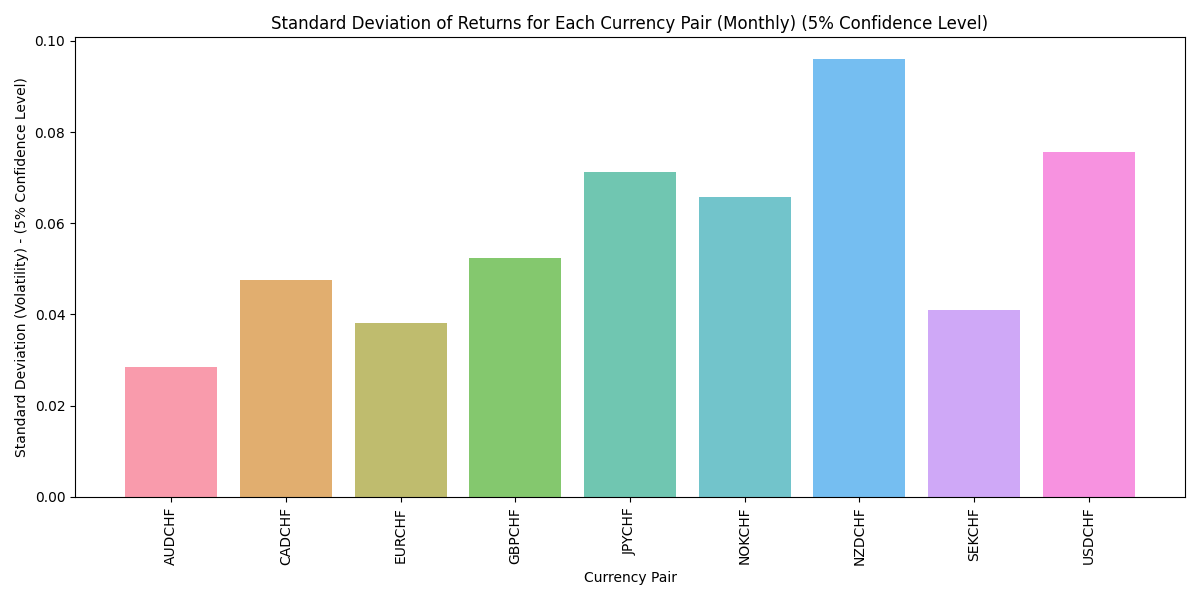
\includegraphics[width=0.75\linewidth]{../../reports/figures/volatility_plot.png}
    \caption{Standard Deviation of Returns for Each Currency Pair (Monthly).}
    \label{fig:volatility_plot}
\end{figure}

\textbf{Value-at-Risk Analysis}

Figure~\ref{fig:VaR_plot} illustrates the VaR at the 5\% confidence level for each currency pair. VaR indicates the maximum expected loss at the given confidence level. \textbf{NZDCHF} and \textbf{NOKCHF} have the largest negative VaR values at -0.0508 and -0.0506, respectively, implying the highest potential losses. On the other hand, \textbf{EURCHF} displays the smallest absolute VaR, at -0.0265, reflecting the lowest risk exposure among the analyzed currency pairs. This suggests that investors in \textbf{NZDCHF} and \textbf{NOKCHF} should be prepared for significant potential losses, while \textbf{EURCHF} presents a more conservative risk profile.

\begin{figure}[H]
    \centering
    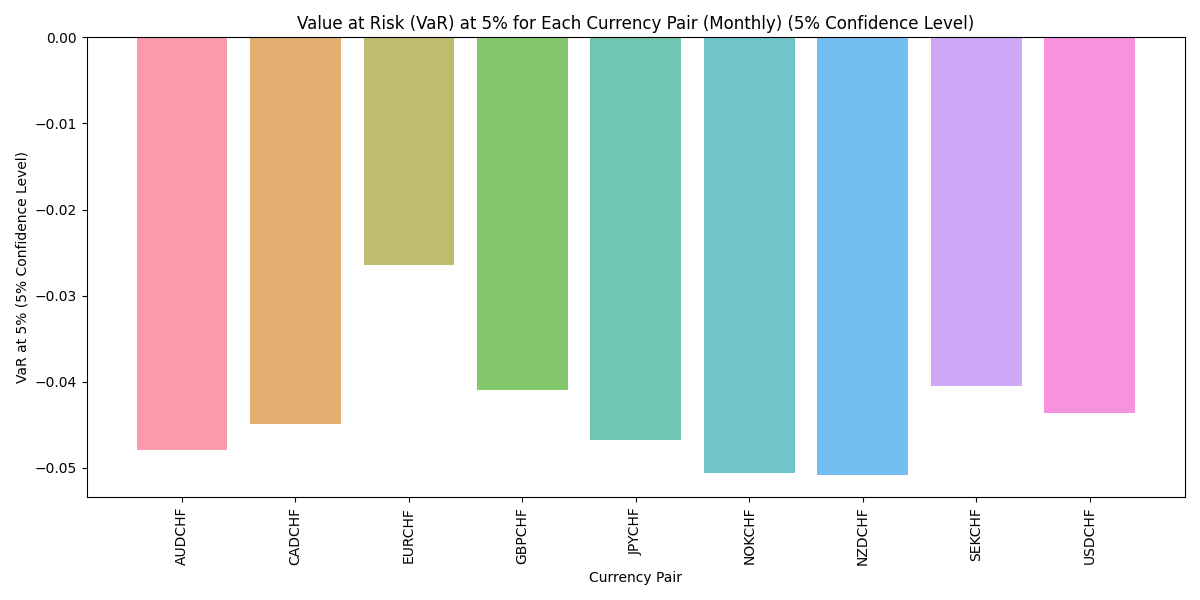
\includegraphics[width=0.75\linewidth]{../../reports/figures/VaR_5_percent_plot.png}
    \caption{Value at Risk at 5\% for Each Currency Pair (Monthly).}
    \label{fig:VaR_plot}
\end{figure}

\textbf{Expected Shortfall Analysis}

Figure~\ref{fig:ES_plot} presents the ES at the 5\% confidence level, representing the average loss in the worst-case scenarios (i.e., losses exceeding the VaR threshold). \textbf{NOKCHF} again shows the largest ES value at -0.076, closely followed by \textbf{CADCHF} at -0.076. These results confirm that these two currency pairs exhibit the highest levels of risk under extreme market conditions. In contrast, \textbf{EURCHF} has the smallest ES at -0.053, further emphasizing its relatively low-risk characteristics.

\begin{figure}[H]
    \centering
    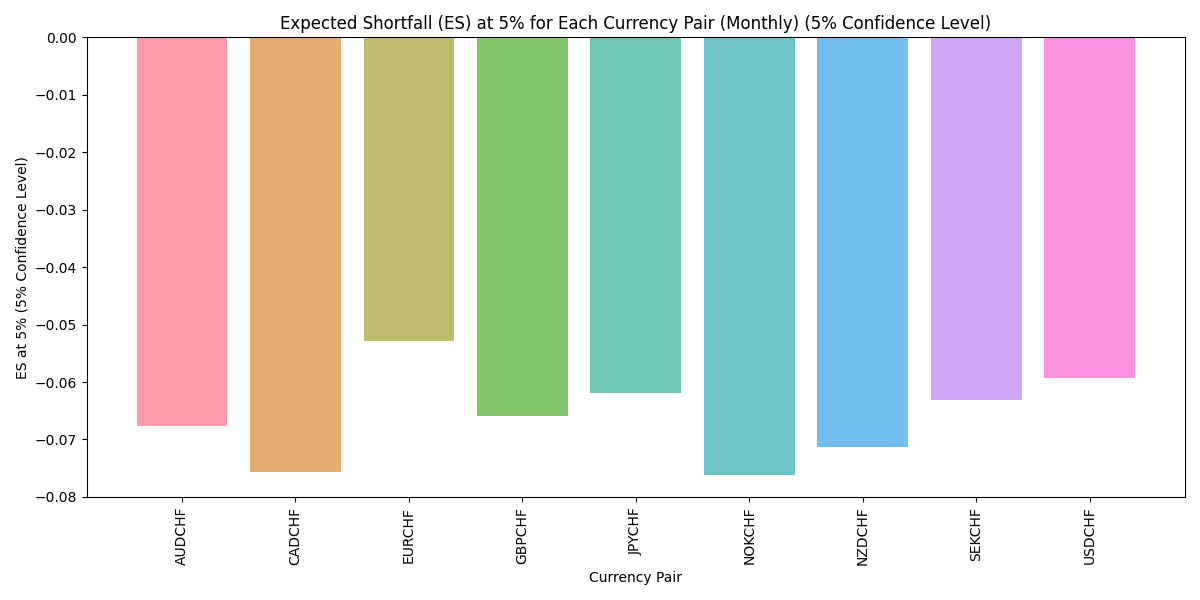
\includegraphics[width=0.75\linewidth]{../../reports/figures/ES_5_percent_plot.png}
    \caption{Expected Shortfall at 5\% for Each Currency Pair (Monthly).}
    \label{fig:ES_plot}
\end{figure}

These results provide critical insights for risk-averse investors and those seeking high-risk, high-return opportunities. For example, \textbf{NZDCHF} and \textbf{NOKCHF} may appeal to investors with a higher risk tolerance, while \textbf{EURCHF} offers a safer alternative for more conservative investment strategies.

\subsection{Daily VaR Calculation}
As a robustness test, the daily VaR measures where estimated via historical data as well as Monte Carlo simulation.

In the historical VaR analysis from Table~\ref{tab:var}, AUDCHF, CADCHF, NOKCHF, and NZDCHF all showed losses exceeding 1\%. 

\begin{table}[H]
\centering
\caption{Historical VaR (5\%) and Monte Carlo VaR (5\%) for each currency pair.} 
\label{tab:var}
\pgfplotstabletypeset[
    col sep=comma,
    fixed zerofill,
    columns/Currency Pair/.style={string type},
    columns/Historical VaR/.style={
        fixed,
        precision=6,
        zerofill
    },
    columns/Monte Carlo VaR/.style={
        fixed,
        precision=6,
        zerofill
    },
    every head row/.style={before row=\hline, after row=\hline},
    every last row/.style={after row=\hline},
]{../../reports/figures/VaR_results.csv}
\end{table}

However, in the Monte Carlo simulation, only AUD and NZD still indicated a VaR loss of over 1\%, suggesting that AUD and NZD exhibited high risk persistence as can be shown in Figure~\ref{fig:monte_carlo_var_simulation_AUDCHF_vs_CHF} and Figure~\ref{fig:monte_carlo_var_simulation_NZDCHF_vs_CHF}.

\begin{figure}[H]
    \centering   
    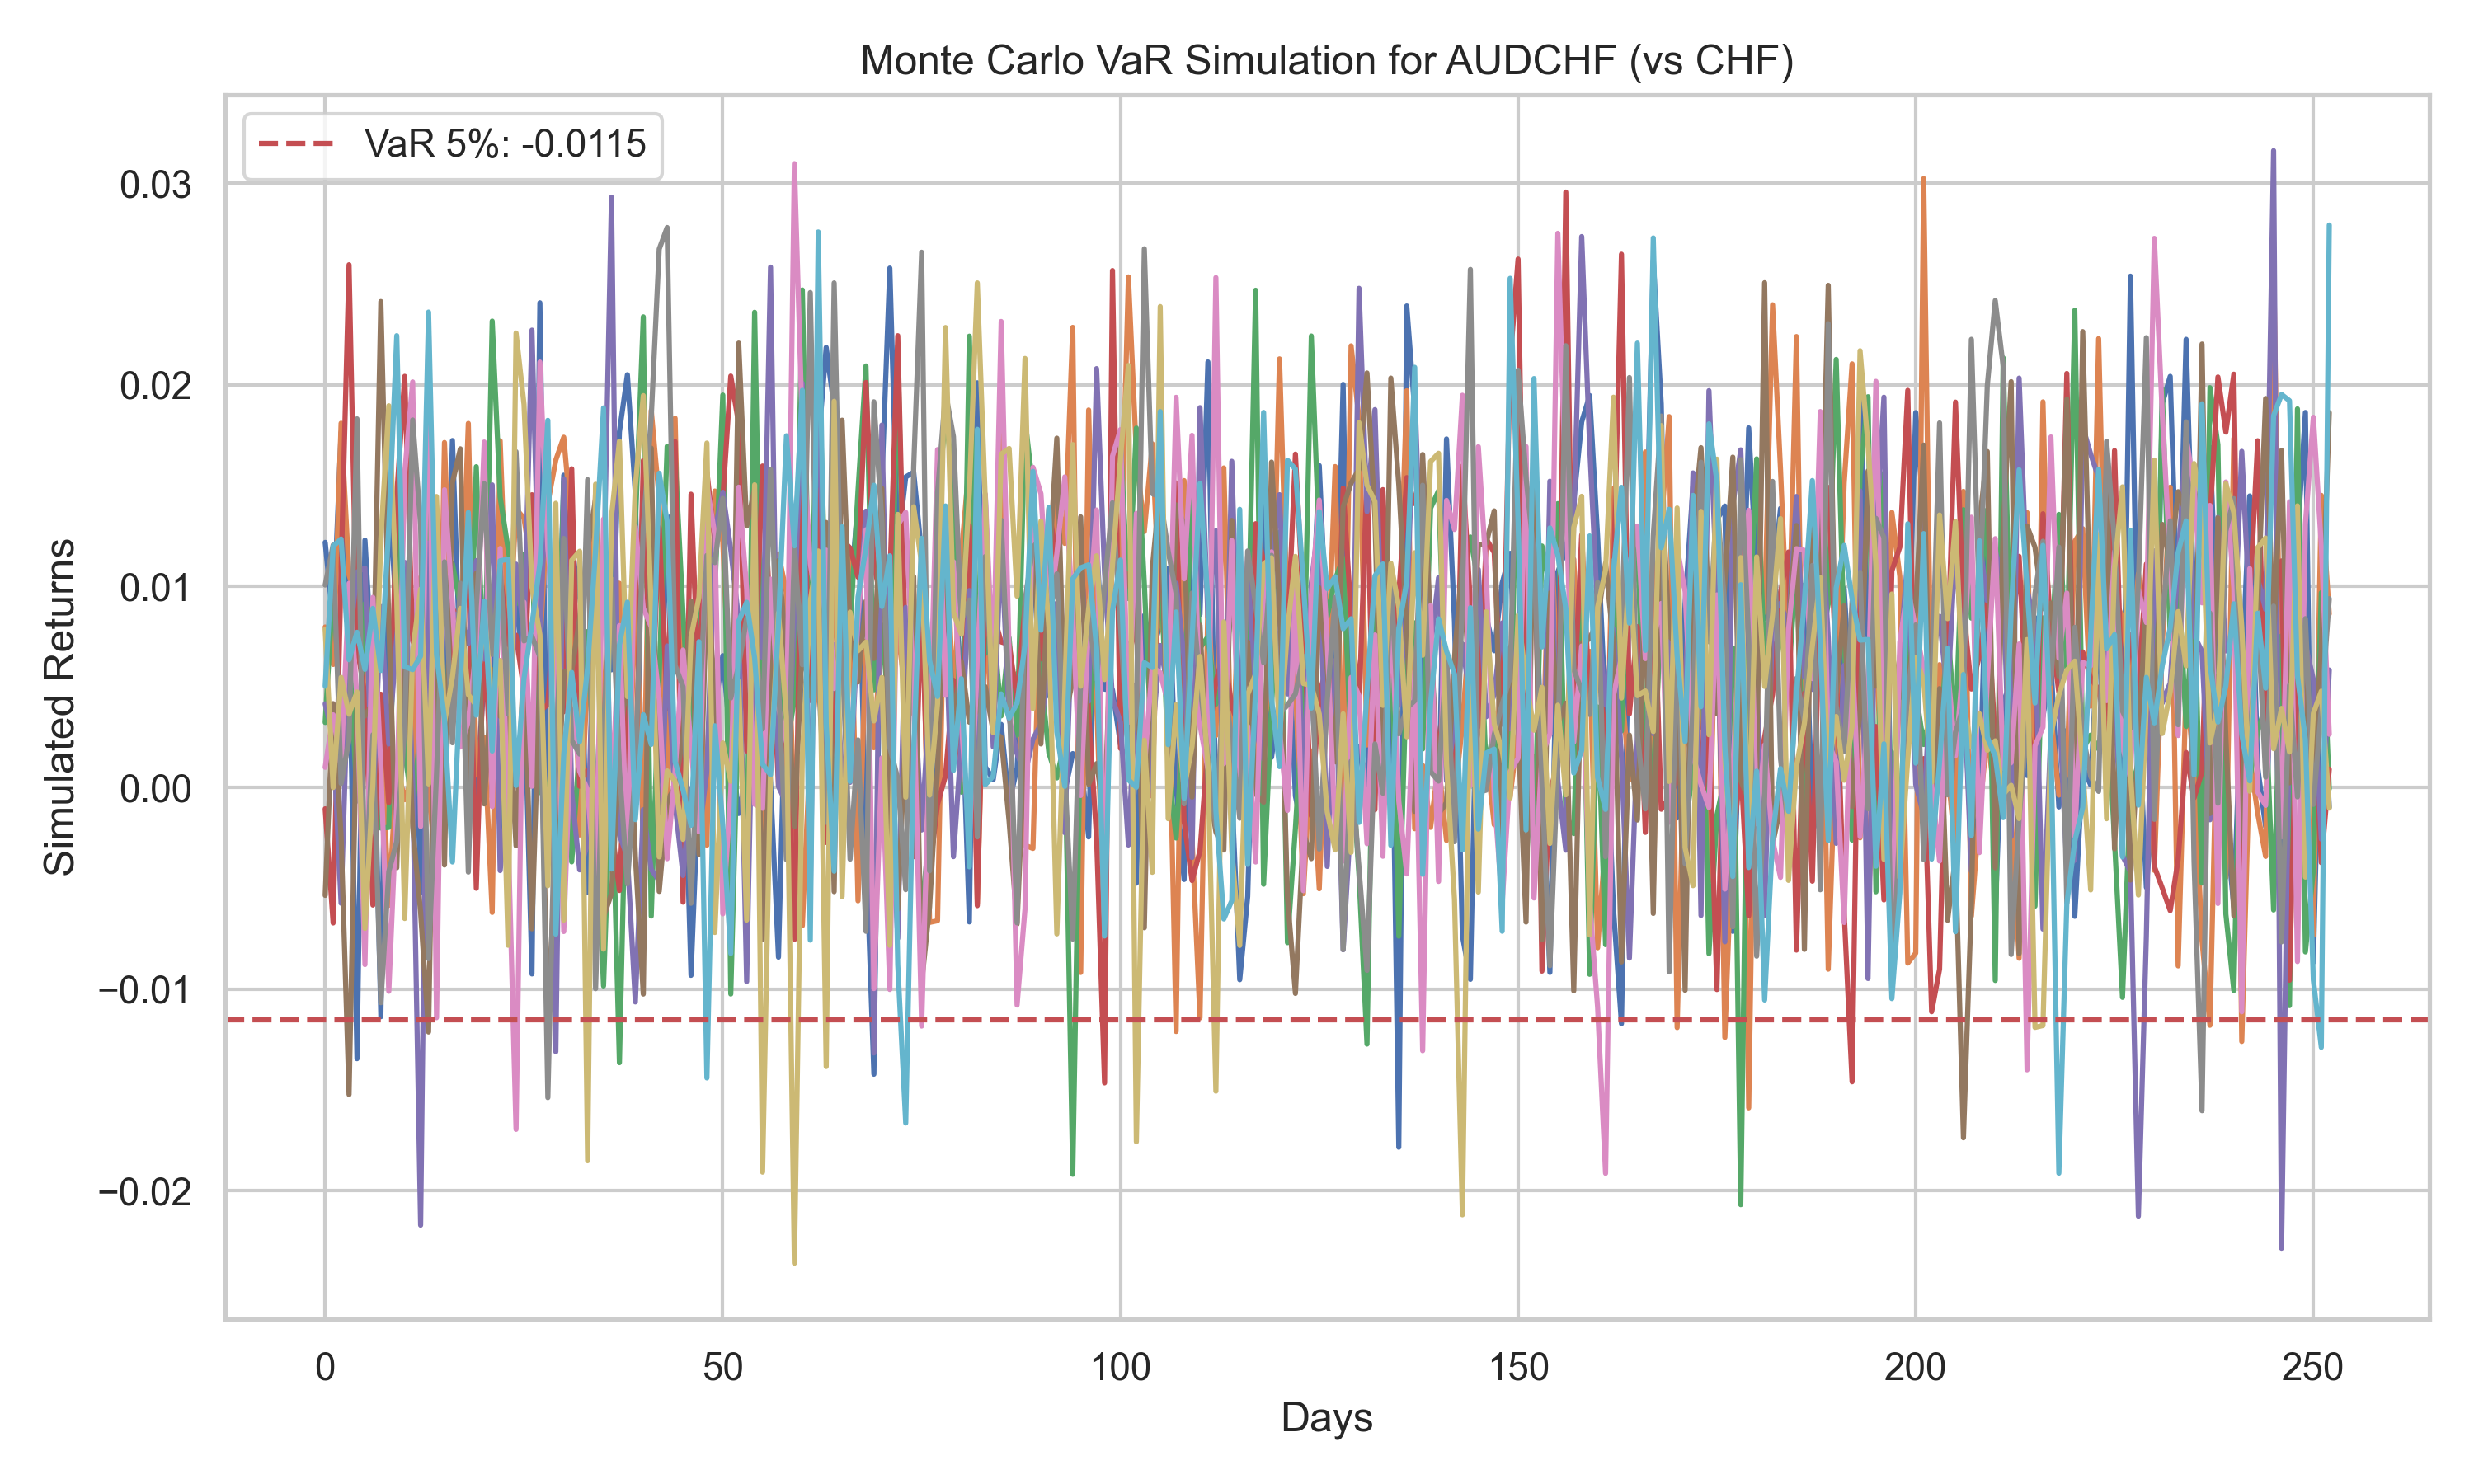
\includegraphics[width=0.75\linewidth]{../../reports/figures/monte_carlo_var_simulation_AUDCHF_vs_CHF.png}
    \caption{Monte Carlo VaR Simulation of AUDCHF vs. CHF}  \label{fig:monte_carlo_var_simulation_AUDCHF_vs_CHF}
\end{figure}

\begin{figure}[H]
    \centering   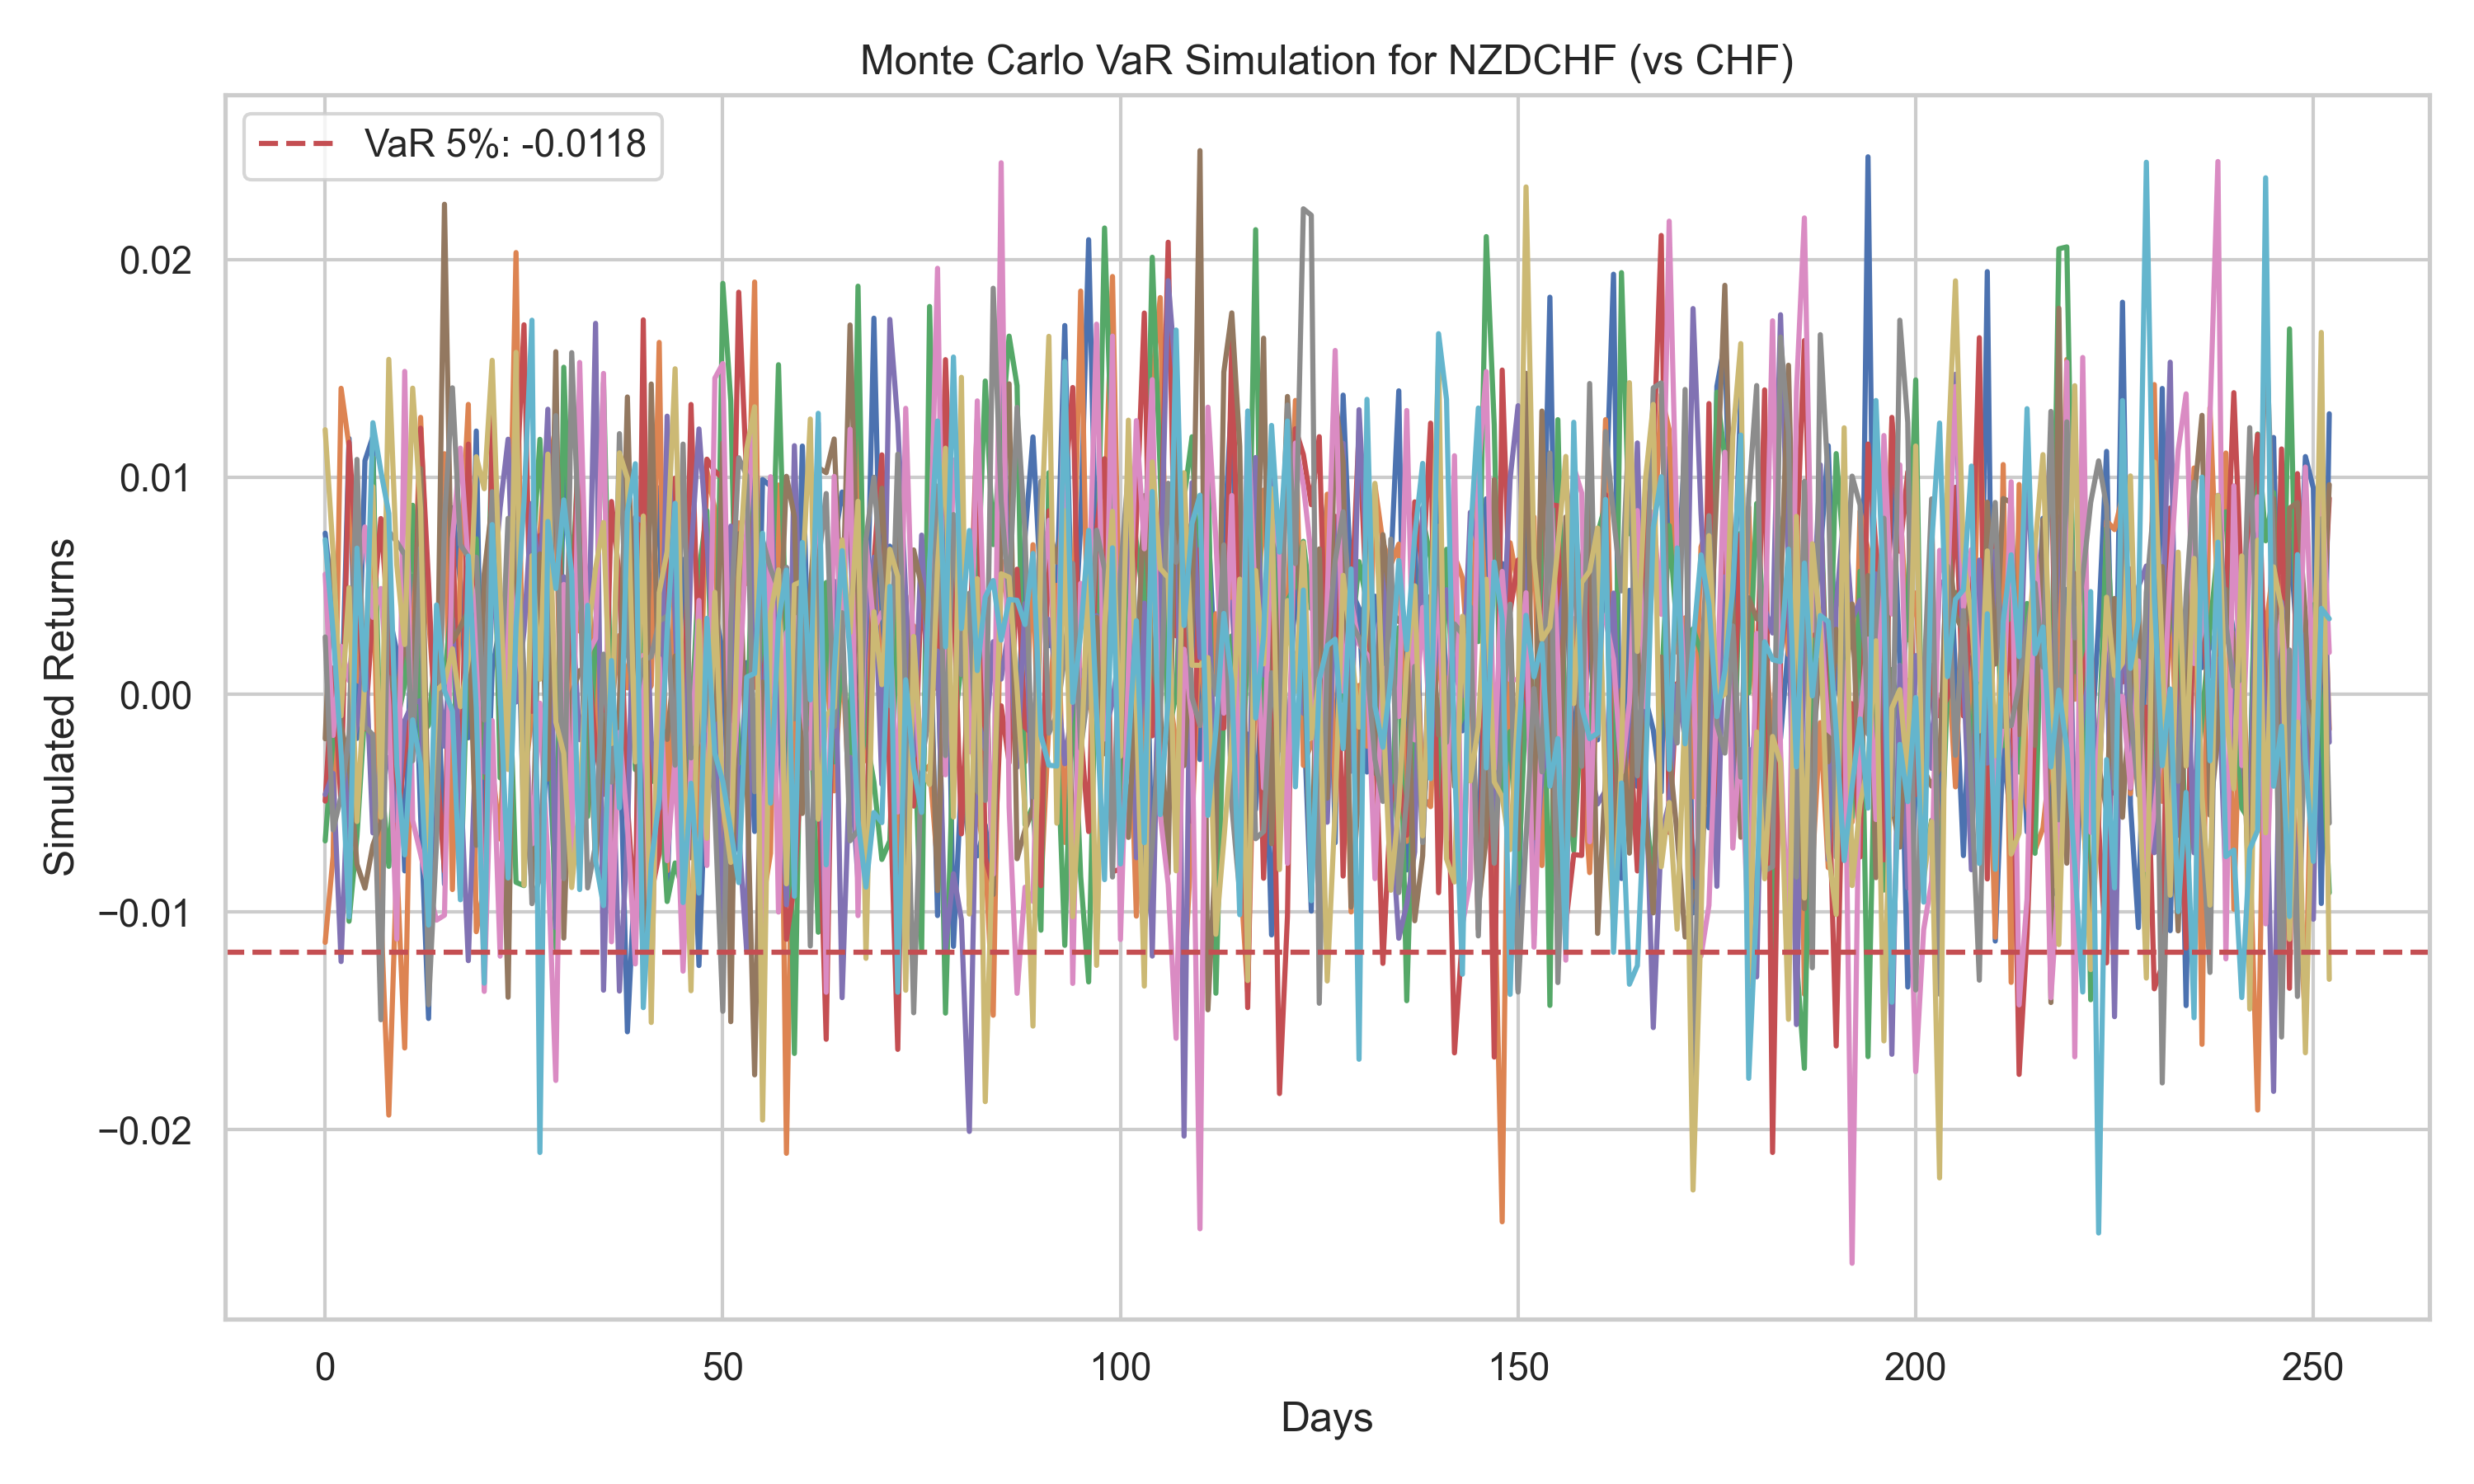
\includegraphics[width=0.75\linewidth]{../../reports/figures/monte_carlo_var_simulation_NZDCHF_vs_CHF.png}
    \caption{Monte Carlo VaR Simulation of NZDCHF vs. CHF}  \label{fig:monte_carlo_var_simulation_NZDCHF_vs_CHF}
\end{figure}

In other words, both historical data and simulations indicated that these two currencies carried sustained risk characteristics, and investors should be particularly cautious when considering these currency pairs. It is worth noting that SEK showed increased risk in the Monte Carlo simulation, with its VaR exceeding 1\%, transitioning from a low-risk to a high-risk profile. This suggested that SEK might face greater uncertainty and potential risks in future market volatility.

\subsection{Daily Price Simulation}
Regarding daily price simulations, GBP showed the most significant price volatility, approximately 0.4 (Figure~\ref{fig:monte_carlo_price_simulation_GBPCHF_vs_CHF}), indicating high future price uncertainty for GBP pairs. 

\begin{figure}[H]
    \centering  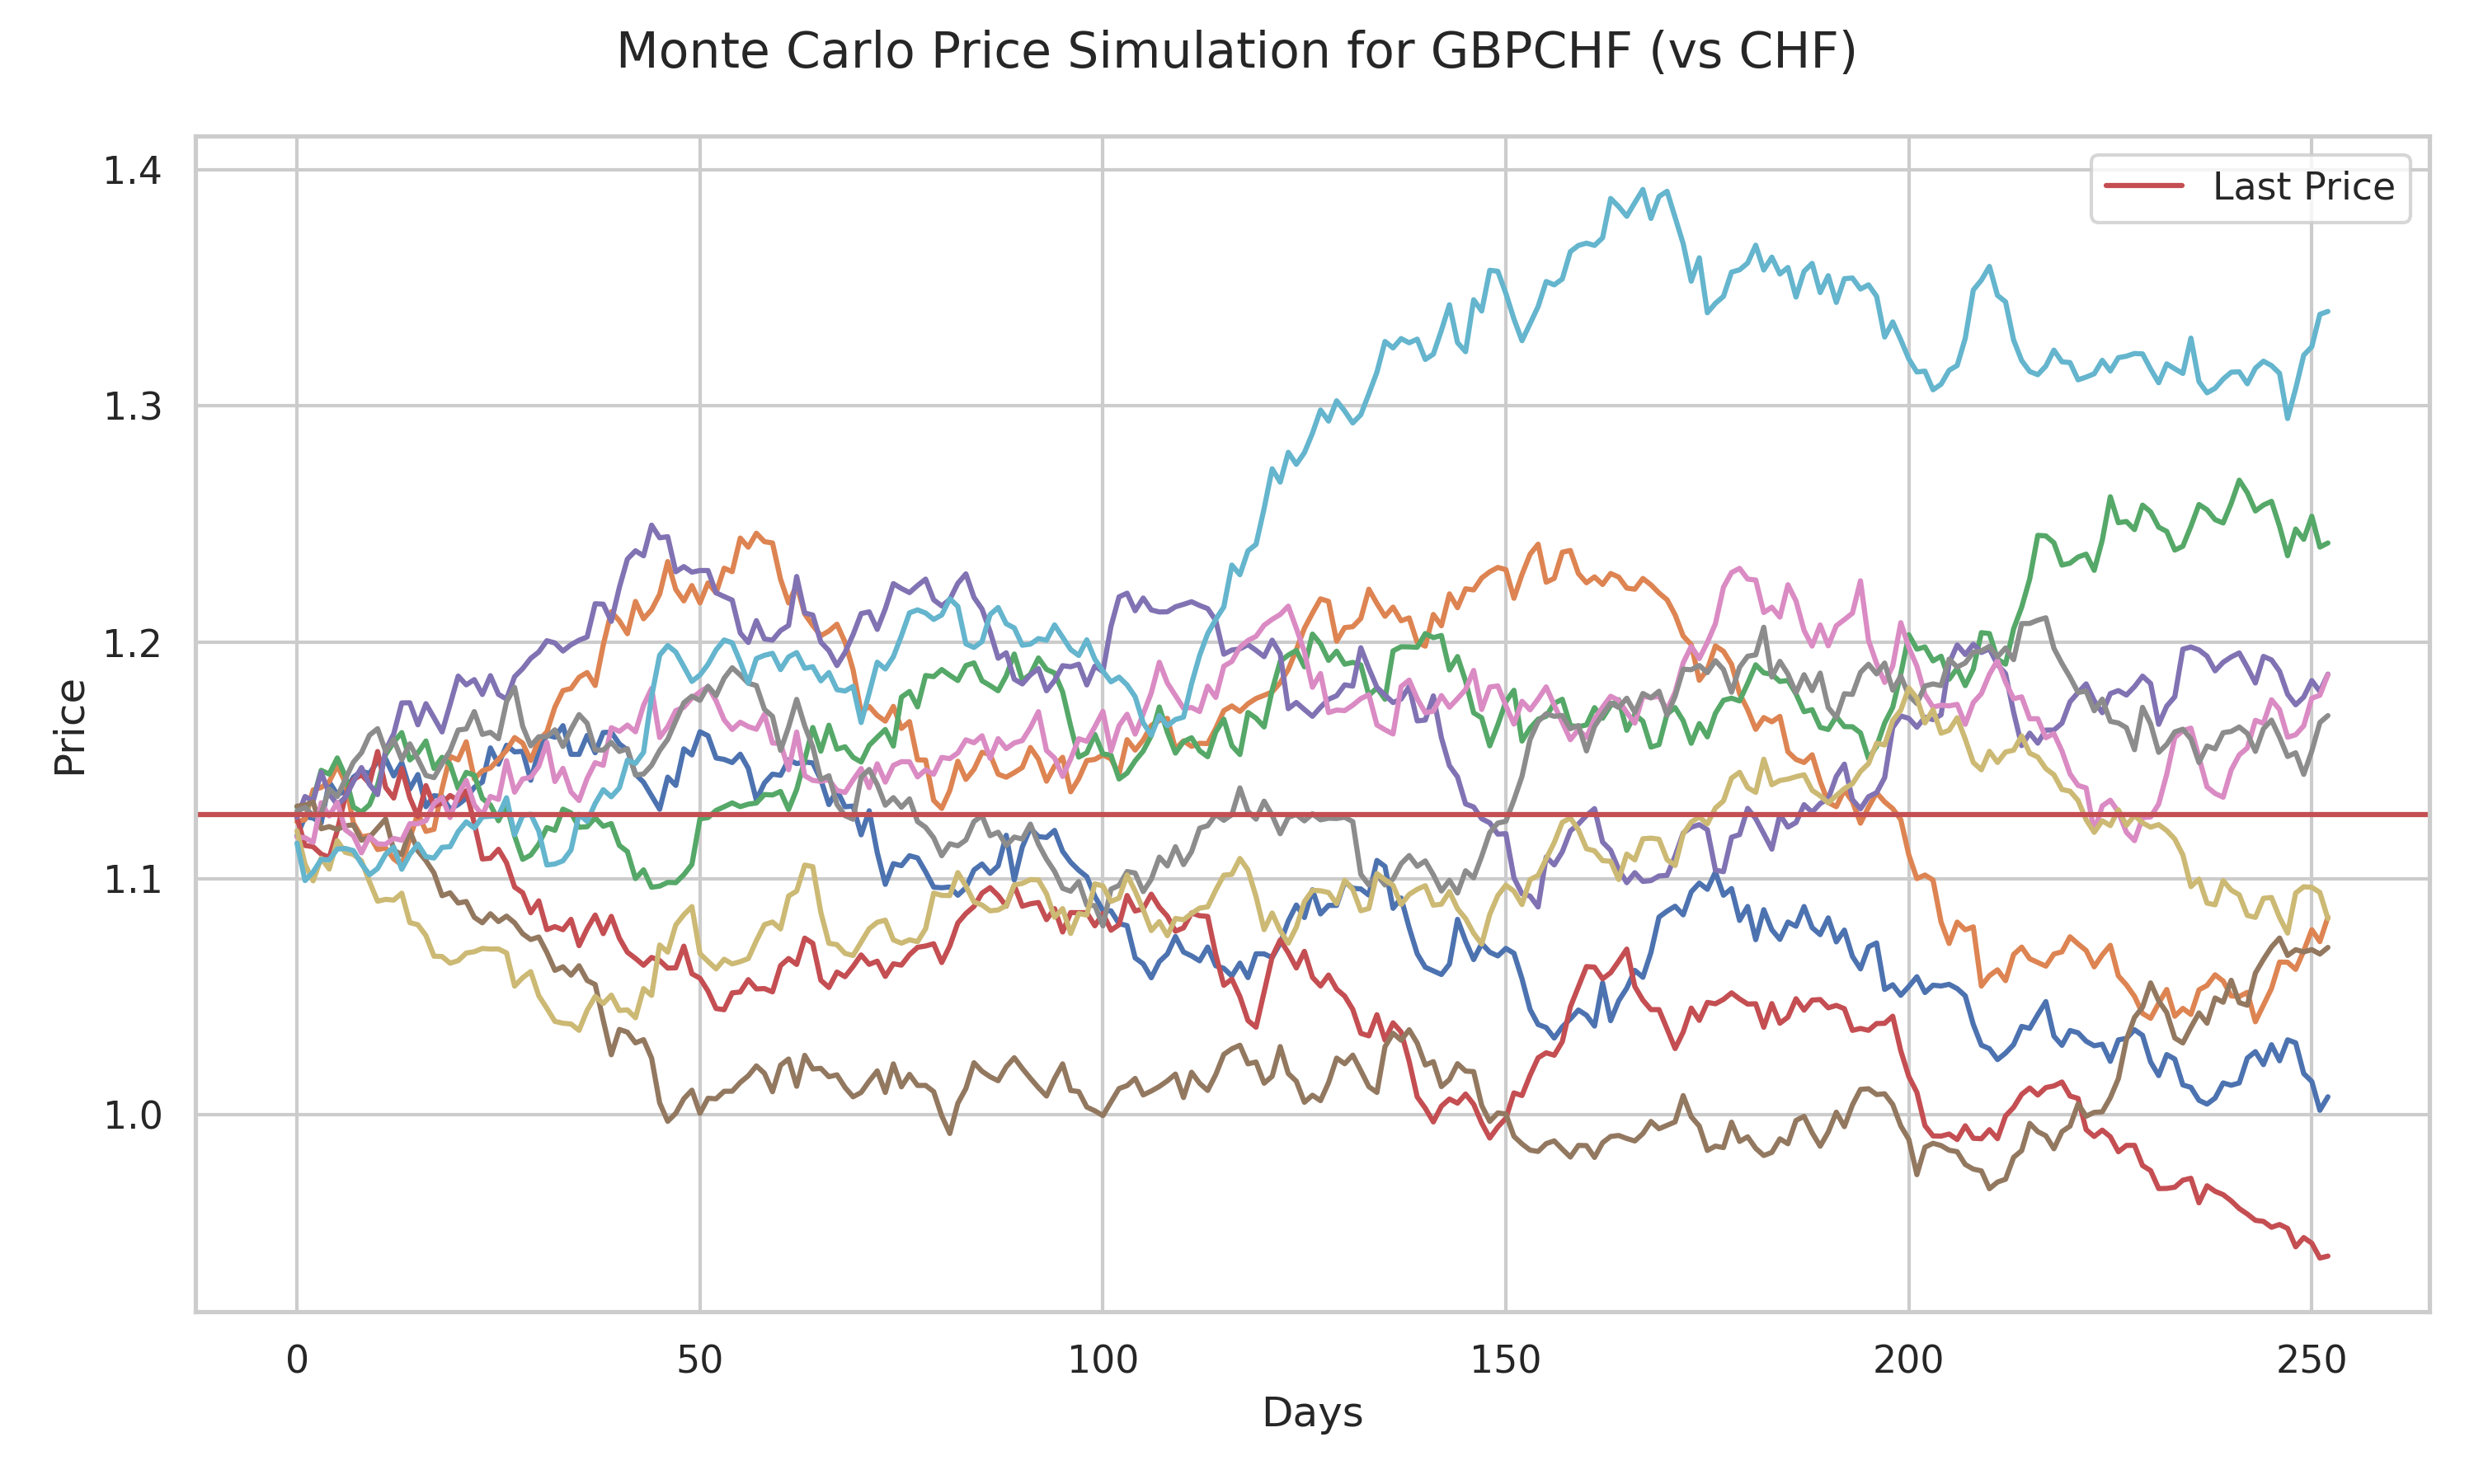
\includegraphics[width=0.75\linewidth]{../../reports/figures/monte_carlo_price_simulation_GBPCHF_vs_CHF.png}
    \caption{Monte Carlo Price Simulation of GBPCHF vs. CHF}  \label{fig:monte_carlo_price_simulation_GBPCHF_vs_CHF}
\end{figure}

Volatility of AUDCHF is around 0.33 (Figure~\ref{fig:monte_carlo_price_simulation_AUDCHF_vs_CHF}), and of NZDCHF is approximately 0.27 (Figure~\ref{fig:monte_carlo_price_simulation_NZDCHF_vs_CHF}), also reflecting considerable price uncertainty. 

\begin{figure}[H]
    \centering 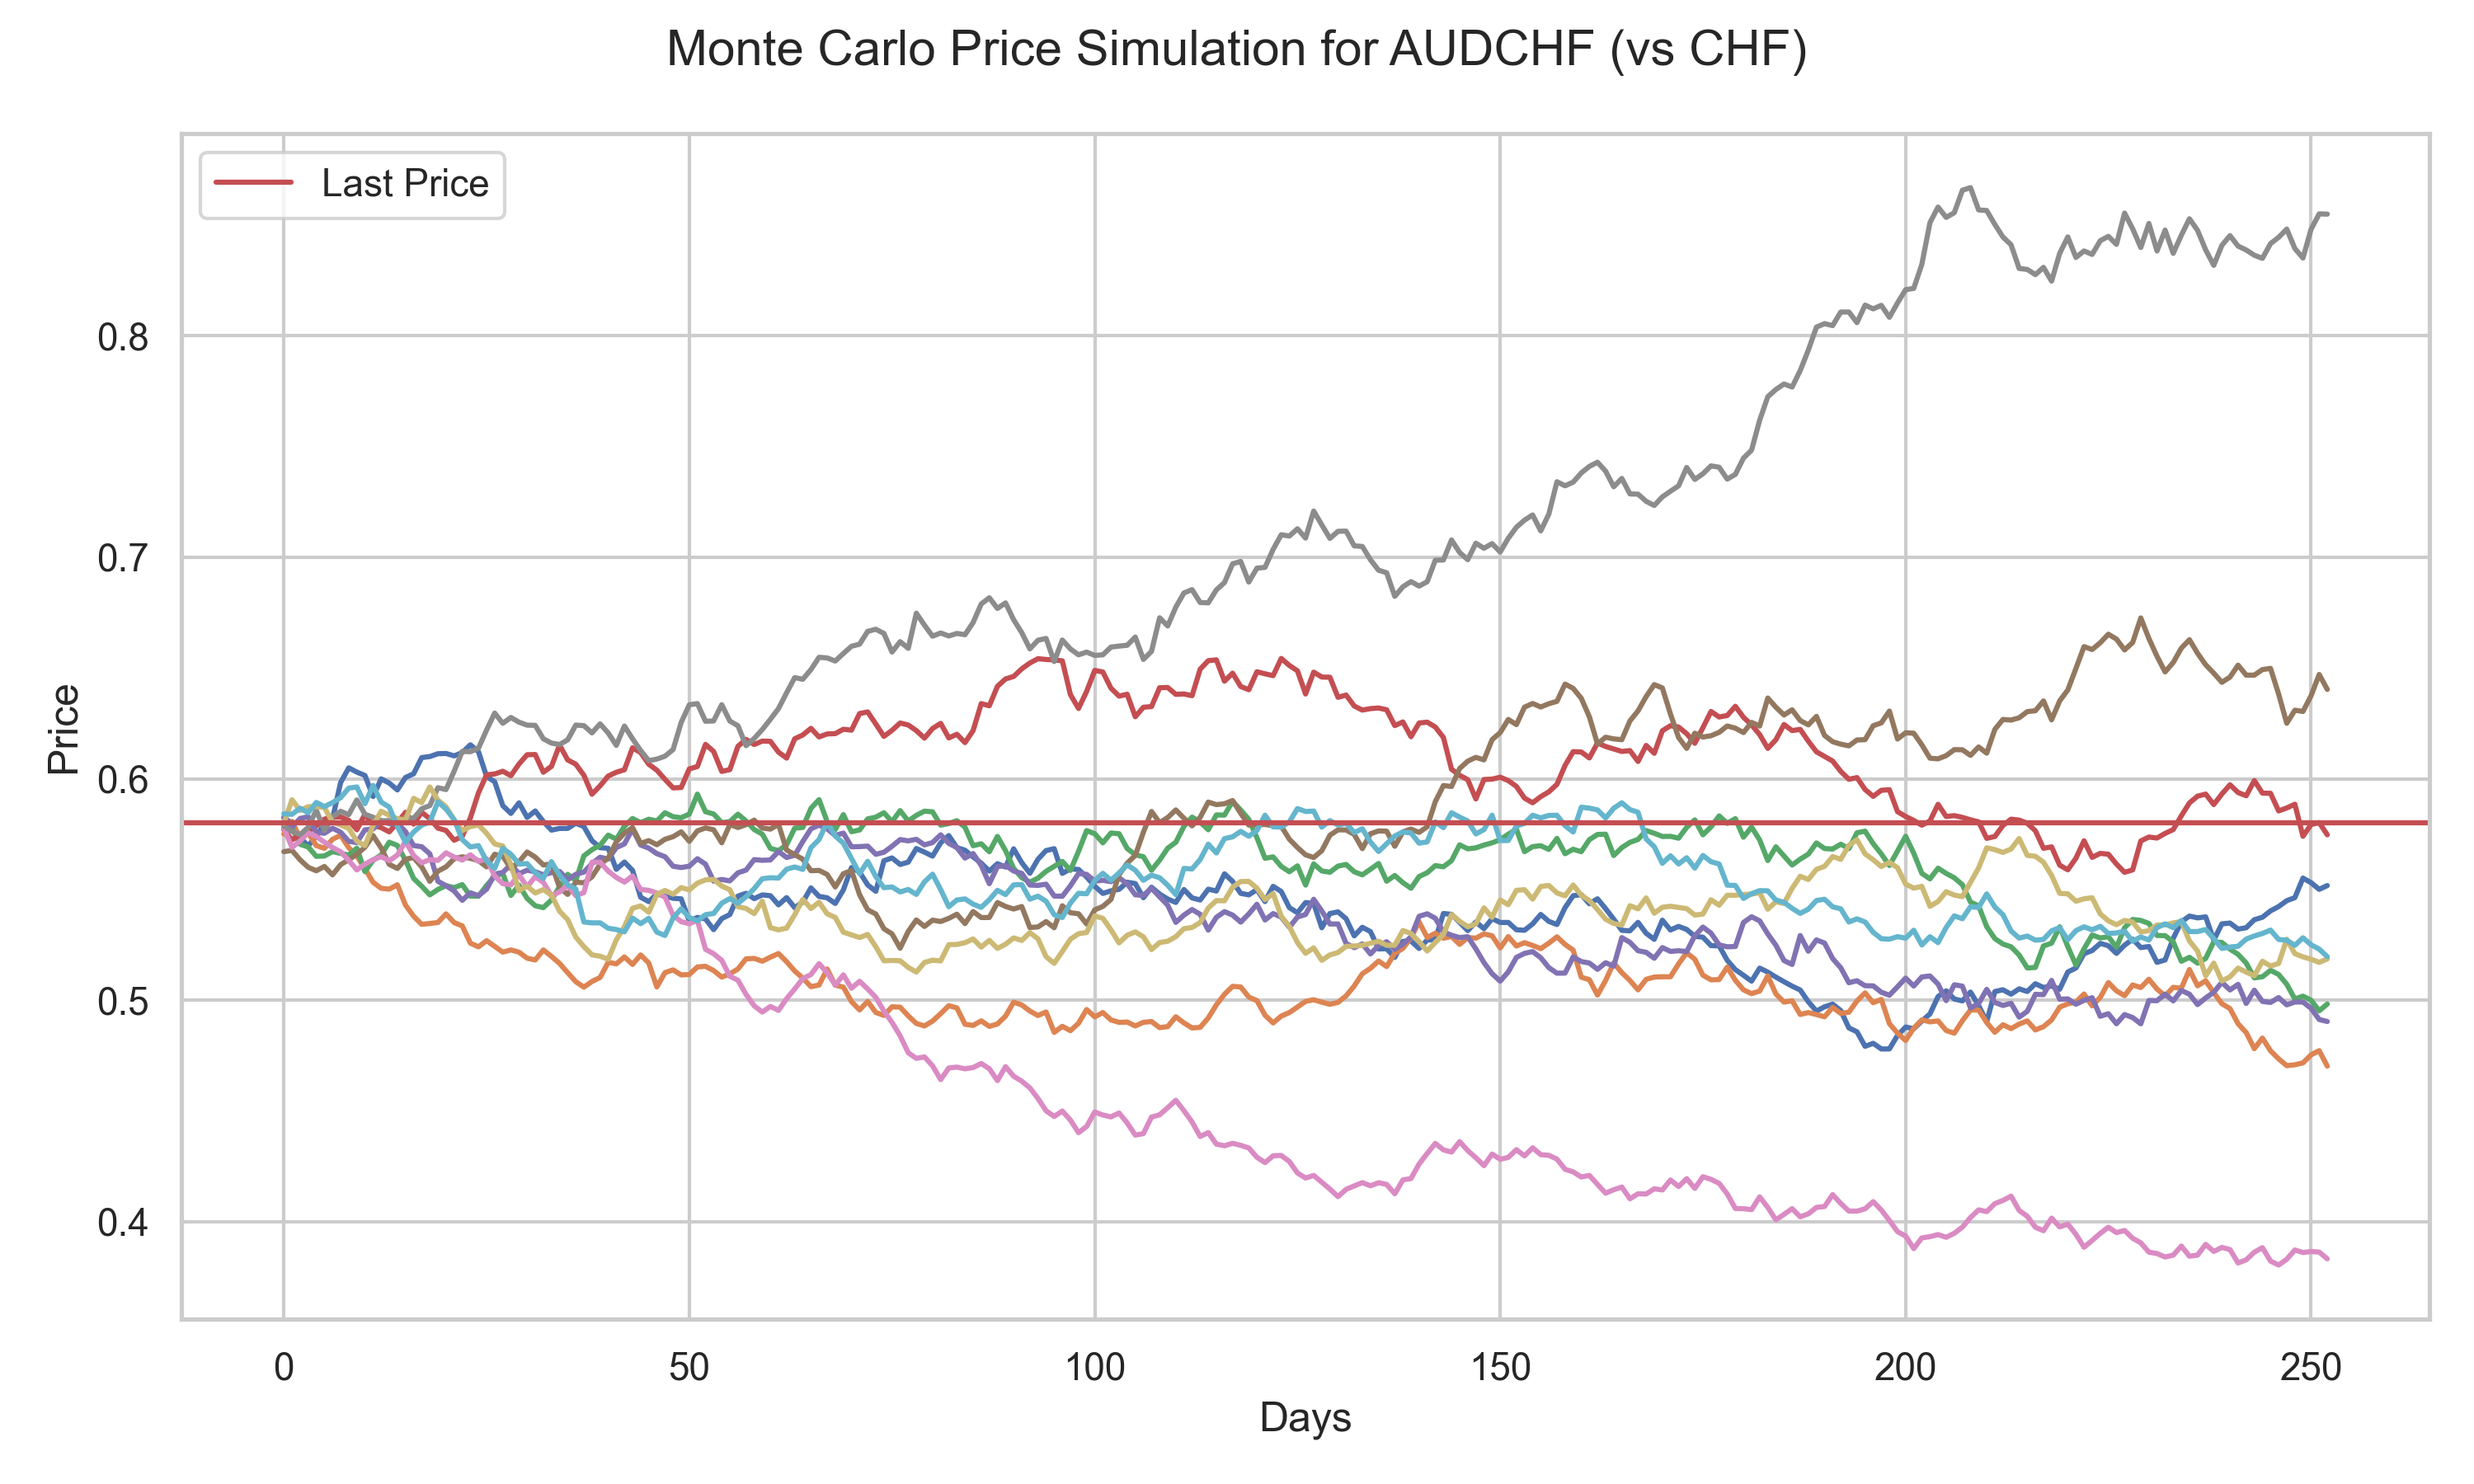
\includegraphics[width=0.75\linewidth]{../../reports/figures/monte_carlo_price_simulation_AUDCHF_vs_CHF.png}
    \caption{Monte Carlo Price Simulation of AUDCHF vs. CHF} \label{fig:monte_carlo_price_simulation_AUDCHF_vs_CHF}
\end{figure}

\begin{figure}[H]
    \centering  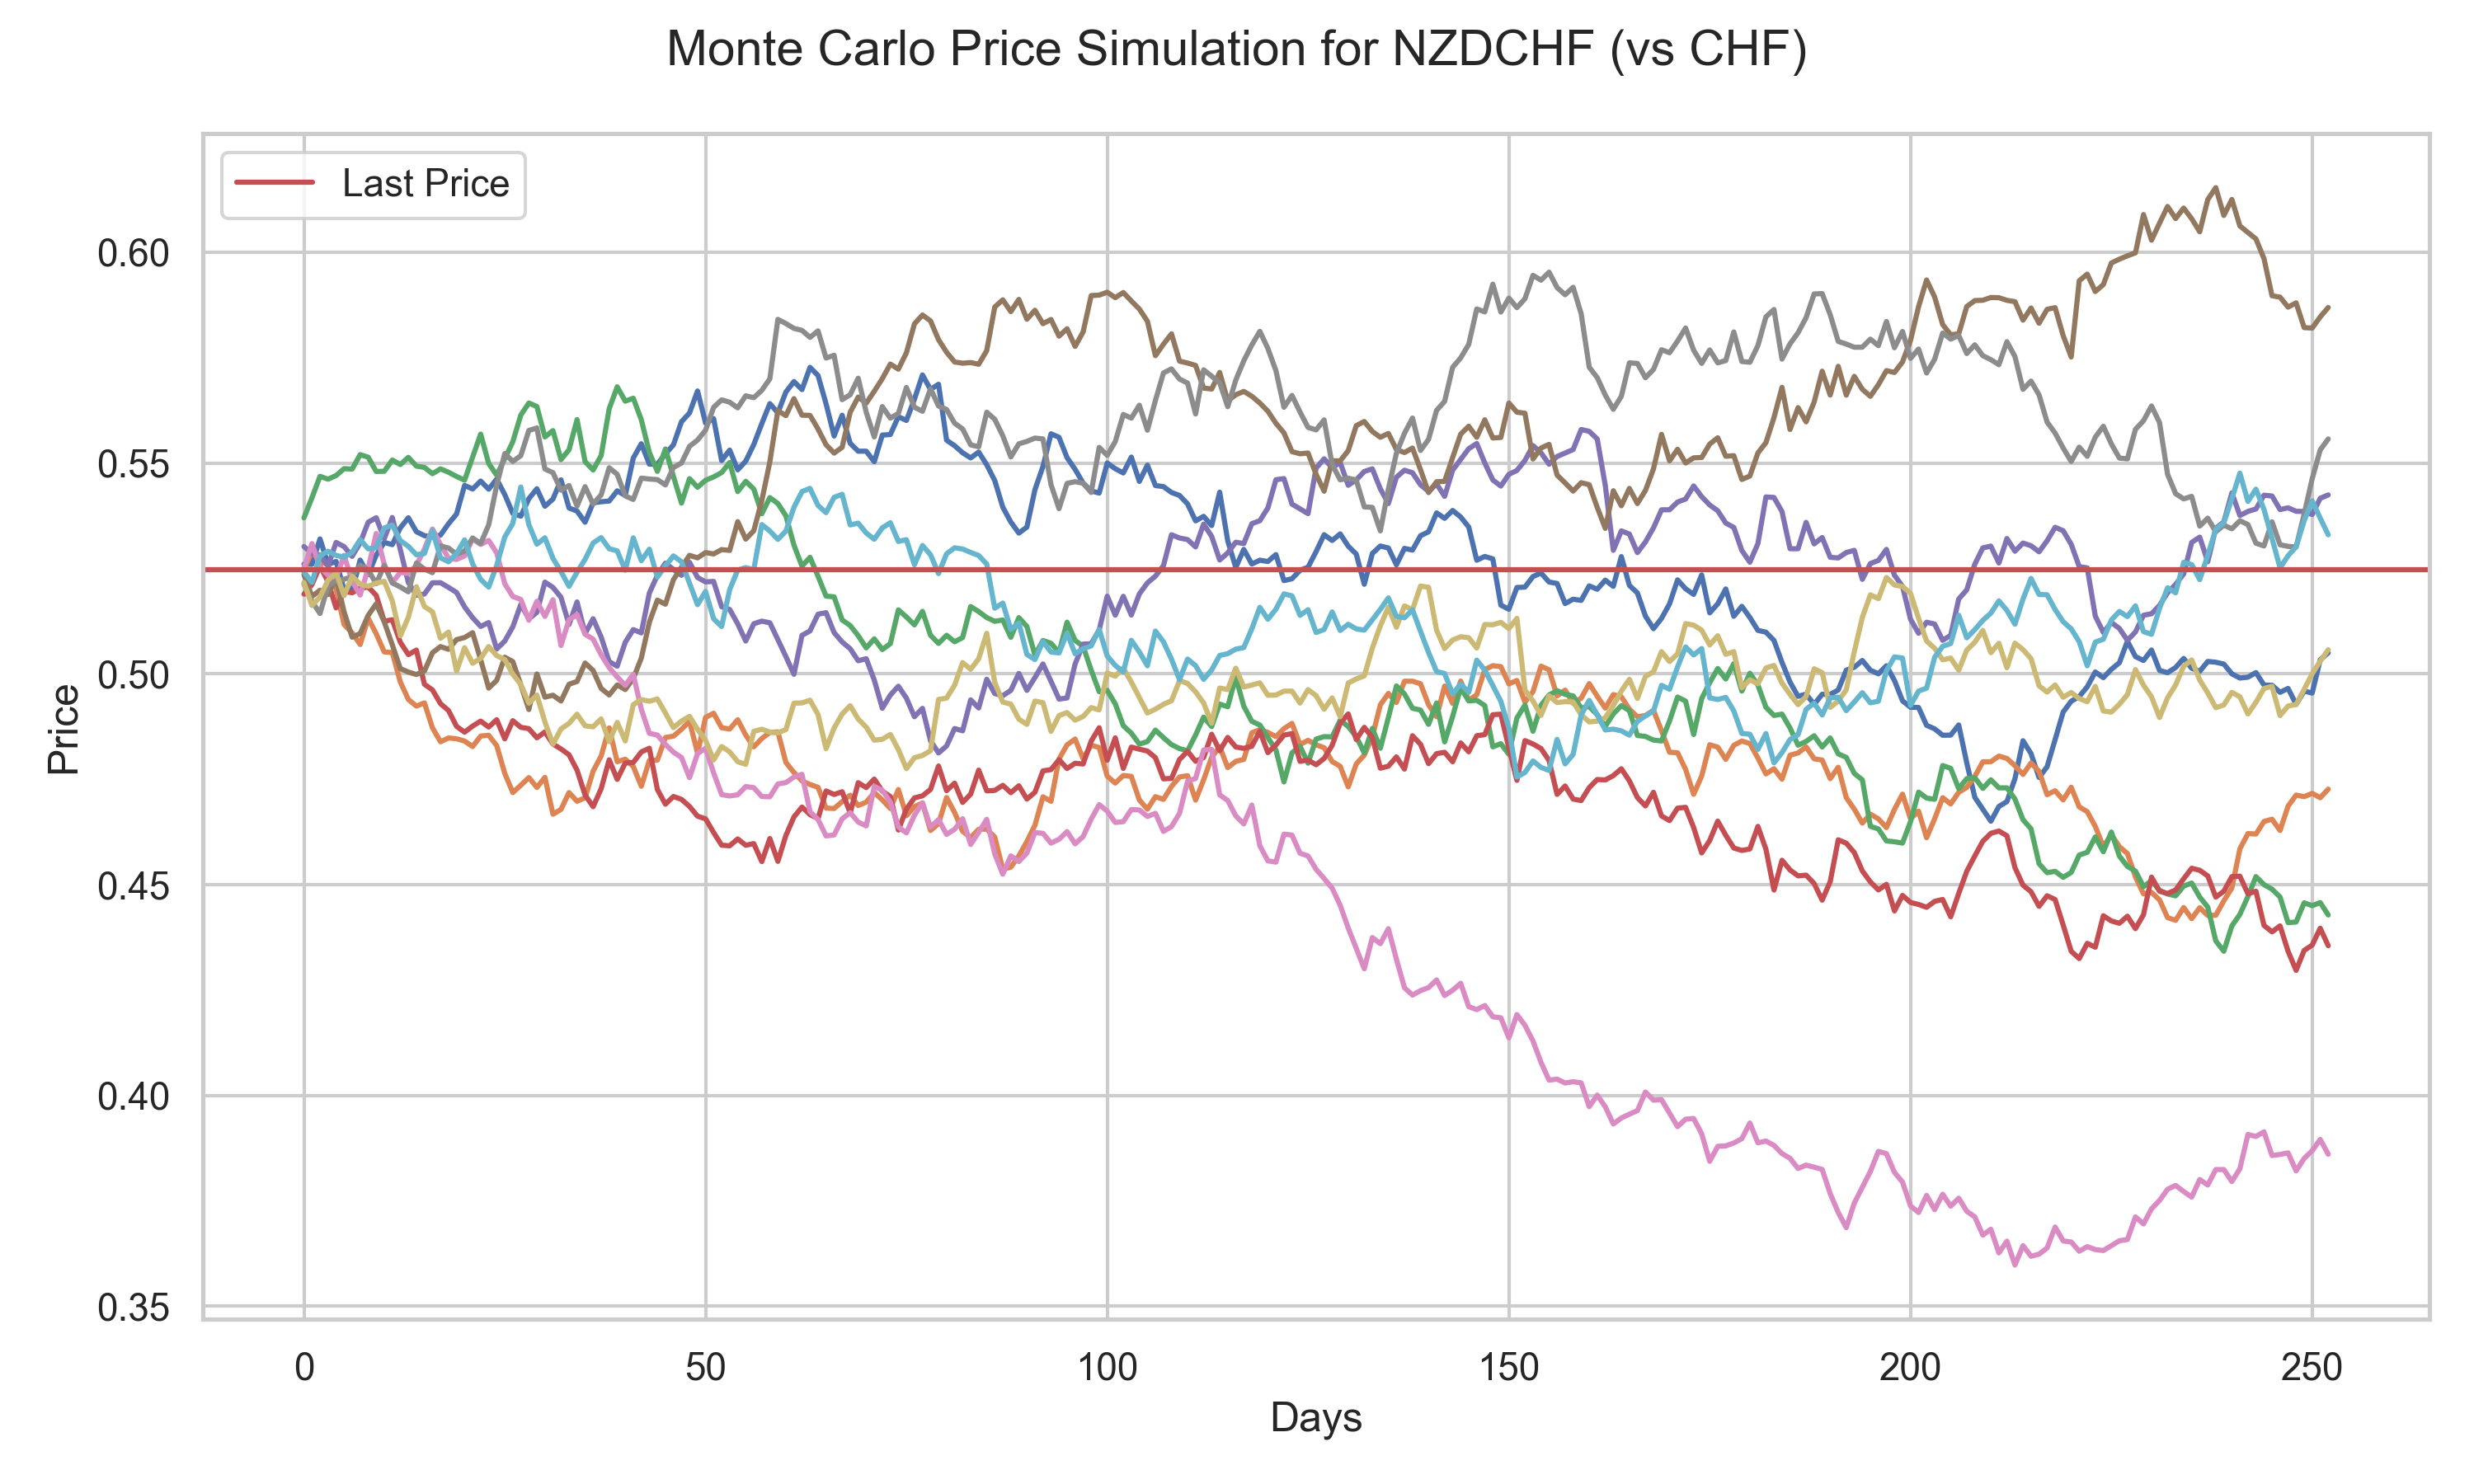
\includegraphics[width=0.75\linewidth]{../../reports/figures/monte_carlo_price_simulation_NZDCHF_vs_CHF.png}
    \caption{Monte Carlo Price Simulation of NZDCHF vs. CHF} \label{fig:monte_carlo_price_simulation_NZDCHF_vs_CHF}
\end{figure}
This suggested that these three currencies have a wide potential price fluctuation range, with correspondingly high investment risks and potential returns.

To summarize the results from both VaR and price simulations, AUD and NZD displayed both high risk persistence and significant price volatility, which means that they were high-risk and high-reward currency pairs suitable only for investors willing to take substantial risks. GBP, despite having a relatively low VaR, had significant price volatility of around 0.4, indicating strong future price fluctuations. Investing in this currency pair requires fully considering the risks associated with its price movements. Therefore, investors should make informed choices regarding these currency pairs based on their own risk tolerance and assessment of future market conditions.

Figure~\ref{fig:monte_carlo_var_simulation_JPYCHF_vs_CHF} and Figure~\ref{fig:monte_carlo_price_simulation_JPYCHF_vs_CHF} showed that JPY had the lowest price volatility, around 0.0022, indicating extremely low future price fluctuations. Combined with its historical VaR and Monte Carlo simulation results consistently remaining around 0.9\%, JPY demonstrated very stable risk characteristics. It could be concluded that JPY is relatively stable in the current market environment. The low volatility and steady VaR make it an excellent hedging option in an investment portfolio, especially suitable for investors seeking lower-risk investments.

\begin{figure}[H]
    \centering  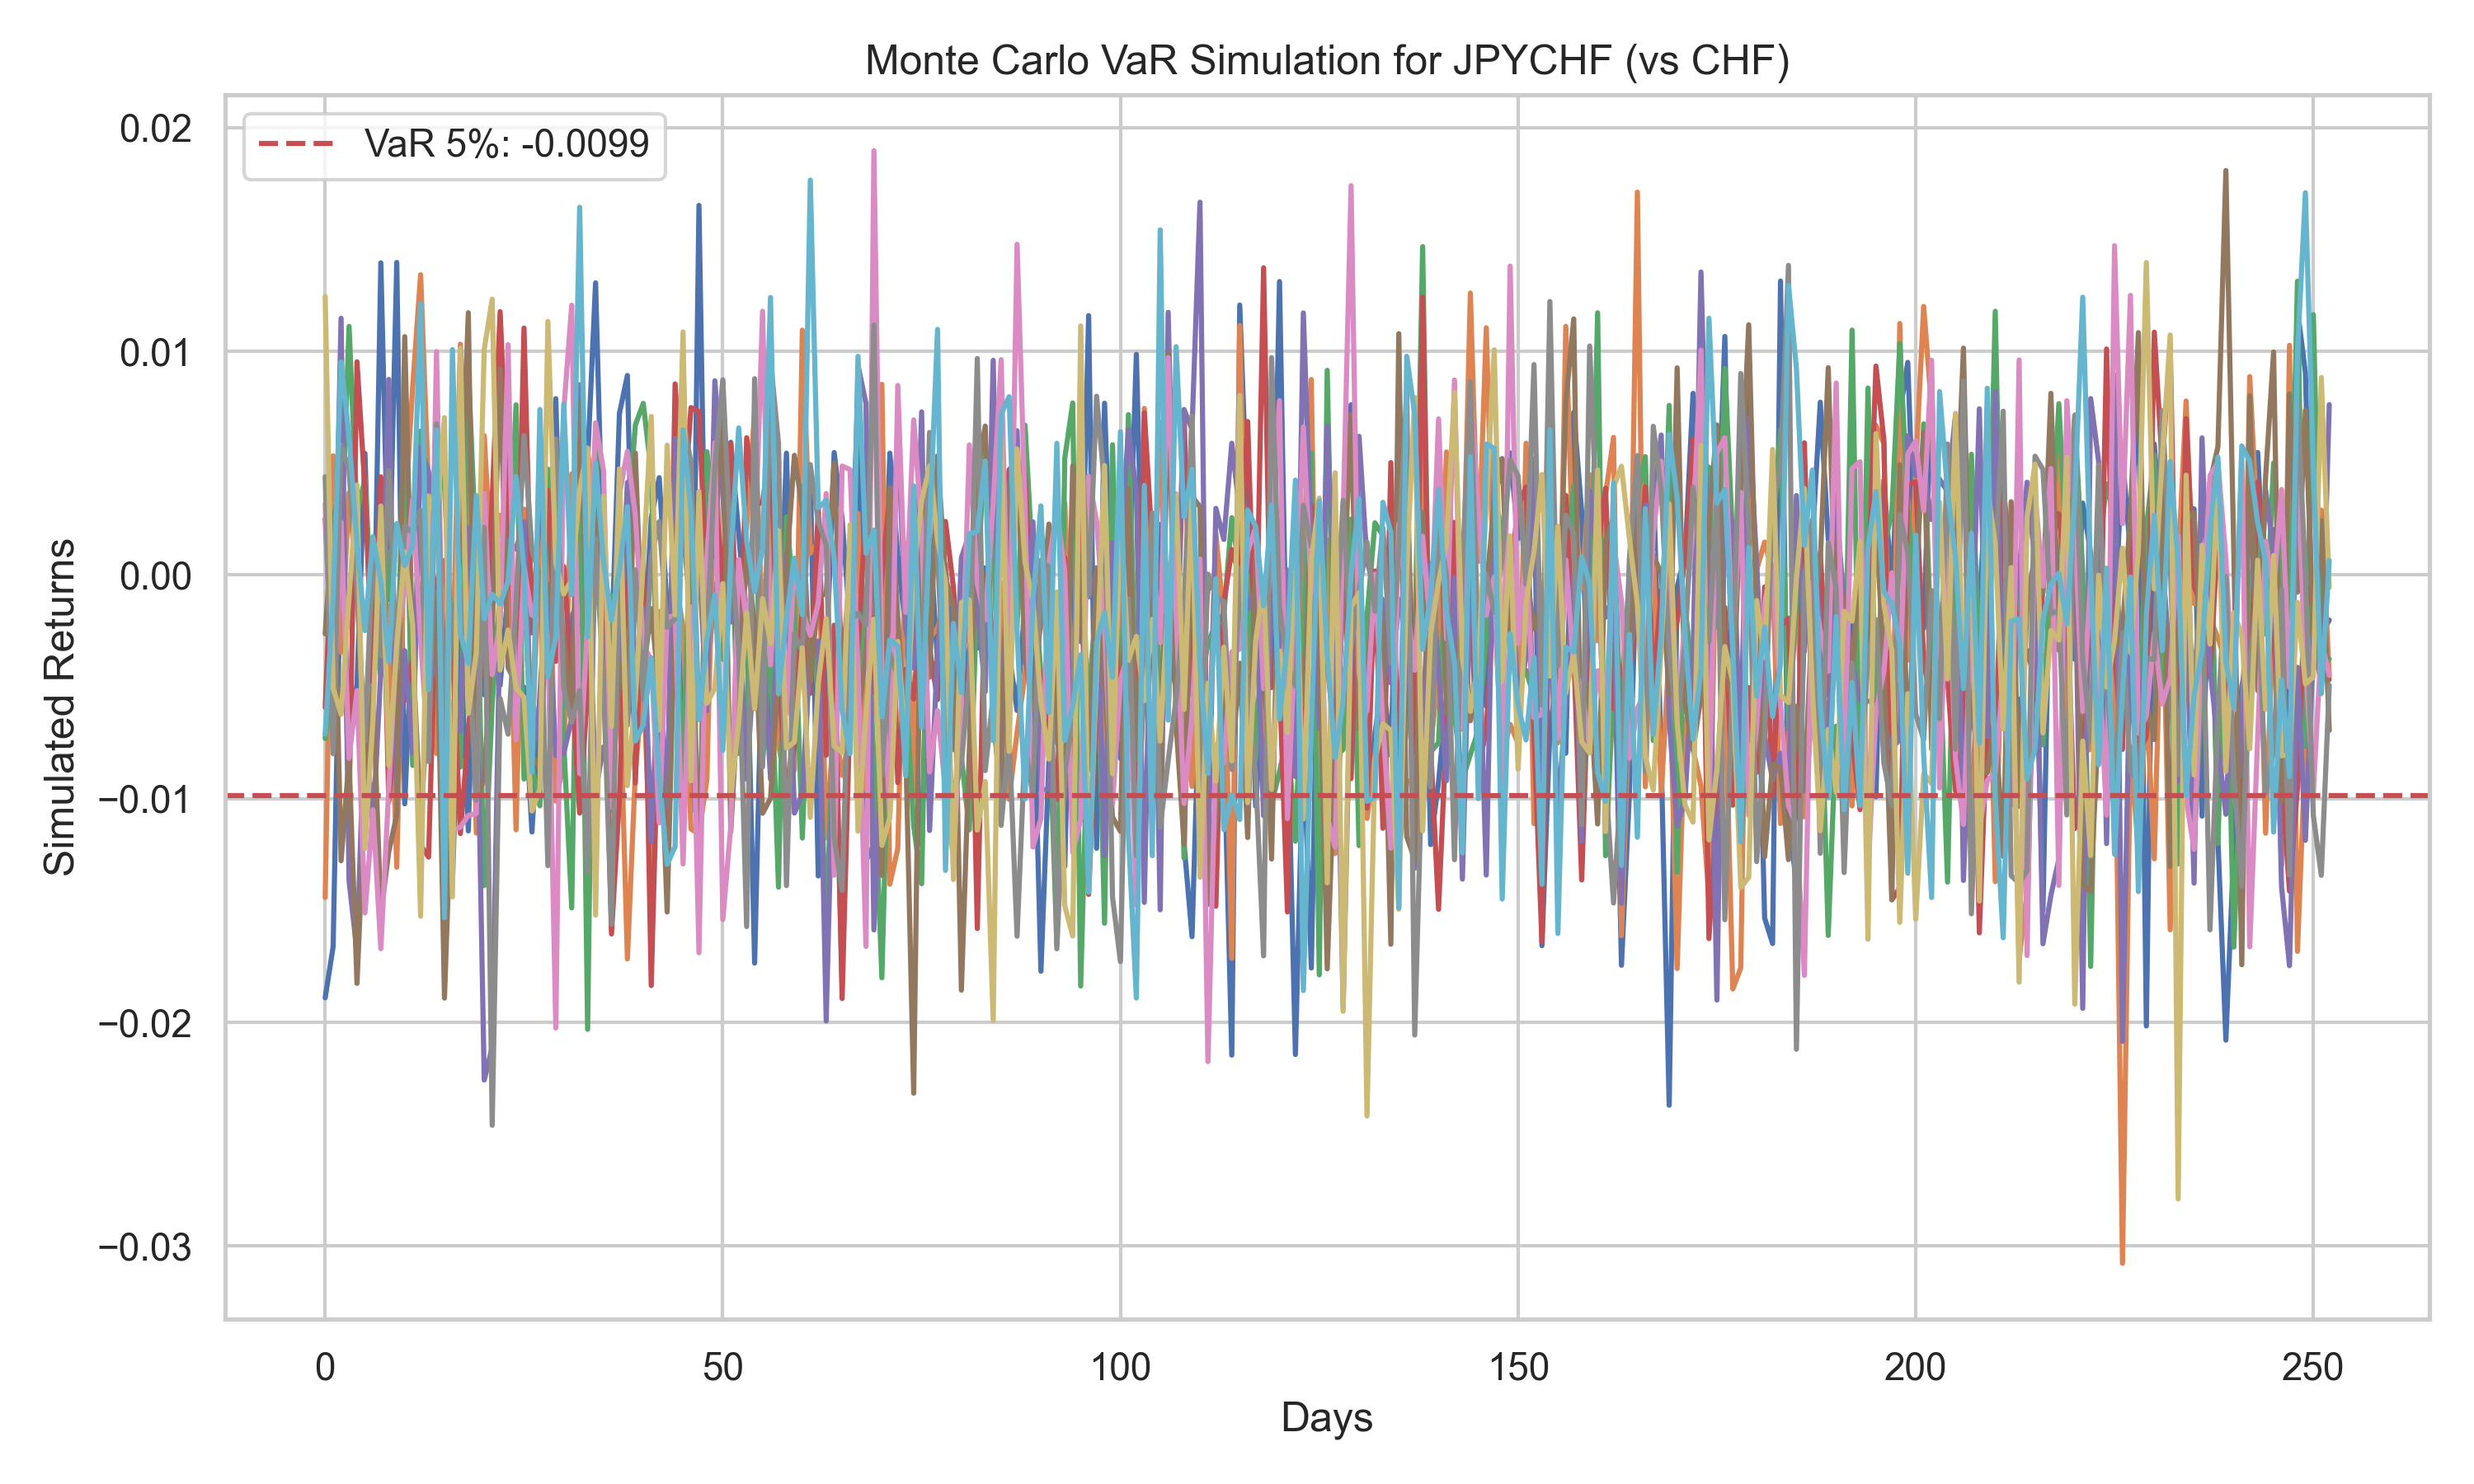
\includegraphics[width=0.75\linewidth]{../../reports/figures/monte_carlo_var_simulation_JPYCHF_vs_CHF.png}
    \caption{Monte Carlo VaR Simulation of JPYCHF vs. CHF}   \label{fig:monte_carlo_var_simulation_JPYCHF_vs_CHF}
\end{figure}

\begin{figure}[H]
    \centering
    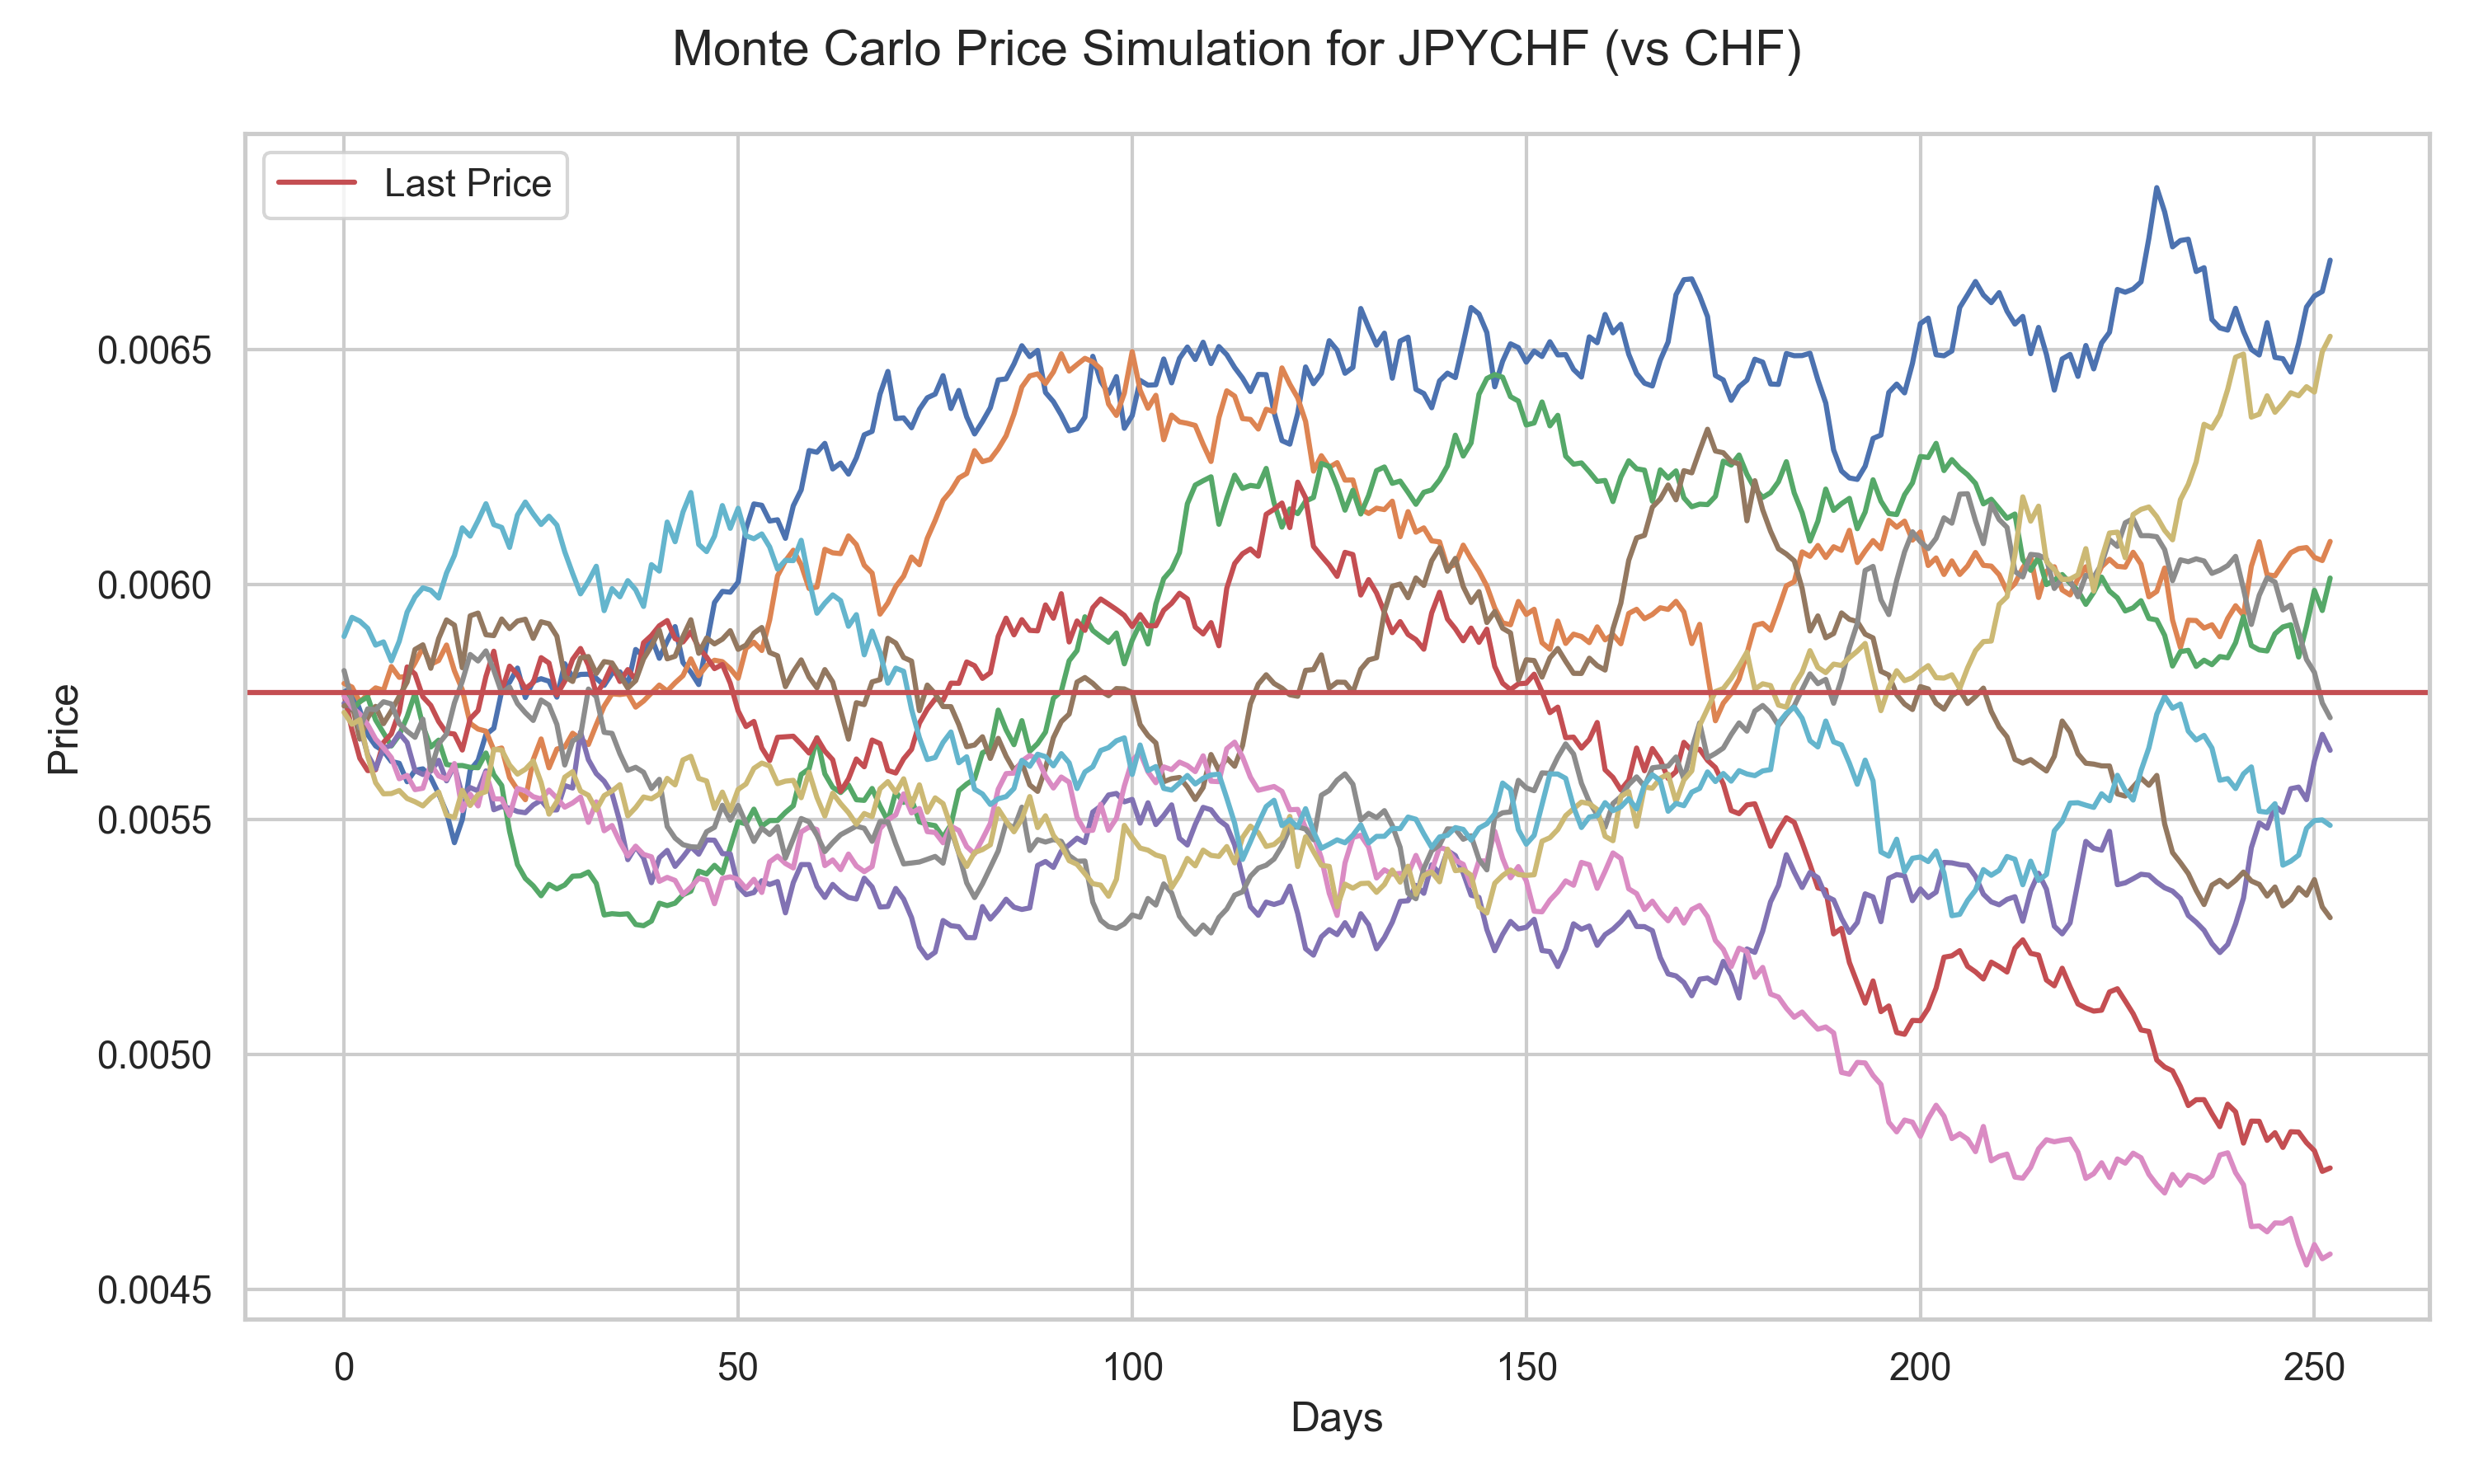
\includegraphics[width=0.75\linewidth]{../../reports/figures/monte_carlo_price_simulation_JPYCHF_vs_CHF.png}
    \caption{Monte Carlo Price Simulation of JPYCHF vs. CHF}  \label{fig:monte_carlo_price_simulation_JPYCHF_vs_CHF}
\end{figure}

\subsection{Interest Rate Regression Analysis}
Under the assumption of uncovered interest parity (UIP), the expected change in the exchange rate should be fully explained by the interest rate differential. In other words, the relationship implies that the exchange rate depreciation (or appreciation) is equal to the difference in the interest rates between the two currencies. According to our model, under the UIP, we would expect $\alpha=0$ and $\beta=-1$.

\begin{table}[H]
\centering
\caption{Regression summaries of exchange rate returns on interest rate differentials.} 
\label{tab:regression}
\resizebox{\textwidth}{!}{
\pgfplotstabletypeset[
    col sep=comma,
    string type,
    columns={Country, Alpha, Beta, Alpha Std.Err., Beta Std.Err., Alpha t, Beta t, Alpha P>|t|, Beta P>|t|},
    columns/Country/.style={string type, column name=Country},
    columns/Alpha/.style={fixed, precision=4, column name=$\alpha$},
    columns/Beta/.style={fixed, precision=4, column name=$\beta$},
    columns/Alpha Std.Err./.style={fixed, precision=4, column name=std.err\_$\alpha$},
    columns/Beta Std.Err./.style={fixed, precision=4, column name=std.err\_$\beta$},
    columns/Alpha t/.style={fixed, precision=4, column name=t-value\_$\alpha$},
    columns/Beta t/.style={fixed, precision=4, column name=t-value\_$\beta$},
    columns/Alpha P>|t|/.style={fixed, precision=4, column name=p-value\_$\alpha$},
    columns/Beta P>|t|/.style={fixed, precision=4, column name=p-value\_$\beta$},
    every head row/.style={before row=\hline, after row=\hline},
    every last row/.style={after row=\hline}
]{../../reports/figures/regression_summaries.csv}
}
\end{table}
The presence of a negative $\alpha$  for all G10 currencies when compared to the CHF implies the existence of a risk premium when holding foreign exchange exposures. In other words, investors appear willing to accept lower returns simply to maintain positions in CHF rather than in other major currencies. This observation underscores the widely recognized role of the CHF as a 'safe-haven' currency. Thanks to 
Switzerland’s longstanding political neutrality, robust financial institutions, and exceptionally low levels of national debt, the CHF is viewed as a particularly stable and low-risk asset. As a result, during periods of pronounced global uncertainty investors gravitate toward the Swiss franc.

Although most results could be deemed statistical significant, beside the issue of multiple testing, there is also nodeling uncertainty. While the results of Australia, Canada, Germany, UK and USA have all a slope coefficient around -1, the results of Japan, Norway, New Zealand and Sweden are likely driven by few extreme ourliers.


\section{Conclusion}

This study aimed to identify the riskiest G10 currencies to hold for Swiss residents by evaluating exchange rate risks using various quantitative methods, including the calculation of VaR, volatility analysis, Monte Carlo simulations, and regression analysis of exchange rate returns on interest rate differentials.

The analysis of basic risk measures revealed that NOK/CHF, NZD/CHF, and AUD/CHF exhibited the highest volatilities among the G10 currency pairs, indicating higher risk due to greater exchange rate fluctuations. 

Historical VaR calculations supported these findings, with AUD/CHF, CAD/CHF, NOK/CHF, and NZD/CHF showing losses exceeding 1\% at the 95\% confidence level. Monte Carlo simulations reinforced the persistent high-risk nature of AUD/CHF and NZD/CHF, as these currency pairs continued to exhibit VaR losses exceeding 1\% in the forward-looking analysis. The price simulations indicated significant future price volatility for GBP/CHF, AUD/CHF, and NZD/CHF, suggesting substantial uncertainty and potential for large fluctuations in exchange rates.

The regression findings indicate that all G10 currencies are likely to offer some degree of risk premium when held in a cash account by a Swiss investor. This conclusion is consistent with the broader notion of the Swiss franc as a safe haven currency. However, the principal aim of this study was to examine the risk associated with G10 currencies, rather than to determine whether that risk is systematically compensated. In order to address the latter, it would also be necessary to consider whether other asset classes, such as equities, provide comparable risk compensation

In conclusion, based on the combined analyses, NZD/CHF consistently emerged as the riskiest currency pair. It exhibited the highest volatility at 0.096, the largest VaR at -0.0508, and significant ES values at -0.0712. NOK/CHF also displayed high risk levels, particularly in terms of VaR (-0.0506) and ES (-0.0762). These findings are supported by the results shown in Figure~\ref{fig:volatility_plot}, Figure~\ref{fig:VaR_plot}, and Figure~\ref{fig:ES_plot}. According to the substantial price uncertainty suggested by Monte Carlo simulations, AUD/CHF also exhibits high risk, primarily due to its elevated volatility and extreme return characteristics.

Investors considering exposure to these currencies should carefully assess their risk tolerance and consider the potential for significant exchange rate fluctuations. Risk management strategies, such as diversification, hedging, or limiting exposure to high-risk currencies, are advisable to mitigate potential adverse impacts on investment portfolios.

On the other hand, JPY/CHF and EUR/CHF appear to be the least risky, exhibiting lower volatility and more stable exchange rate movements against the Swiss Franc. These currencies may be more suitable for risk-averse investors seeking to minimize exchange rate risk in their portfolios. This finding aligns with previous literature, which highlights that some G10 currencies, such as the Swiss Franc and Japanese Yen, exhibit strong safe-haven properties~\cite{ranaldo2010safe}. Furthermore, as a key currency in the Euro Area, the Euro plays an important role in the daily financial activities of Swiss residents~\cite{engel2016exchange}~\cite{goulferni2023switzerland}. The lower volatility between the Euro and Swiss Franc is primarily due to Switzerland's close economic ties with the Eurozone. This consistency with established research further validates the accuracy of our analysis.

Ultimately, the findings of this study underscore the importance for Swiss residents to carefully evaluate the exchange rate risks associated with holding foreign currencies. By employing quantitative risk assessment methods, investors can make more informed decisions and develop effective strategies to manage and mitigate currency risk.


\section*{Appendix}
The appendix includes all the figures in the project that are not mentioned in the main text.

\begin{figure}[H]
    \centering  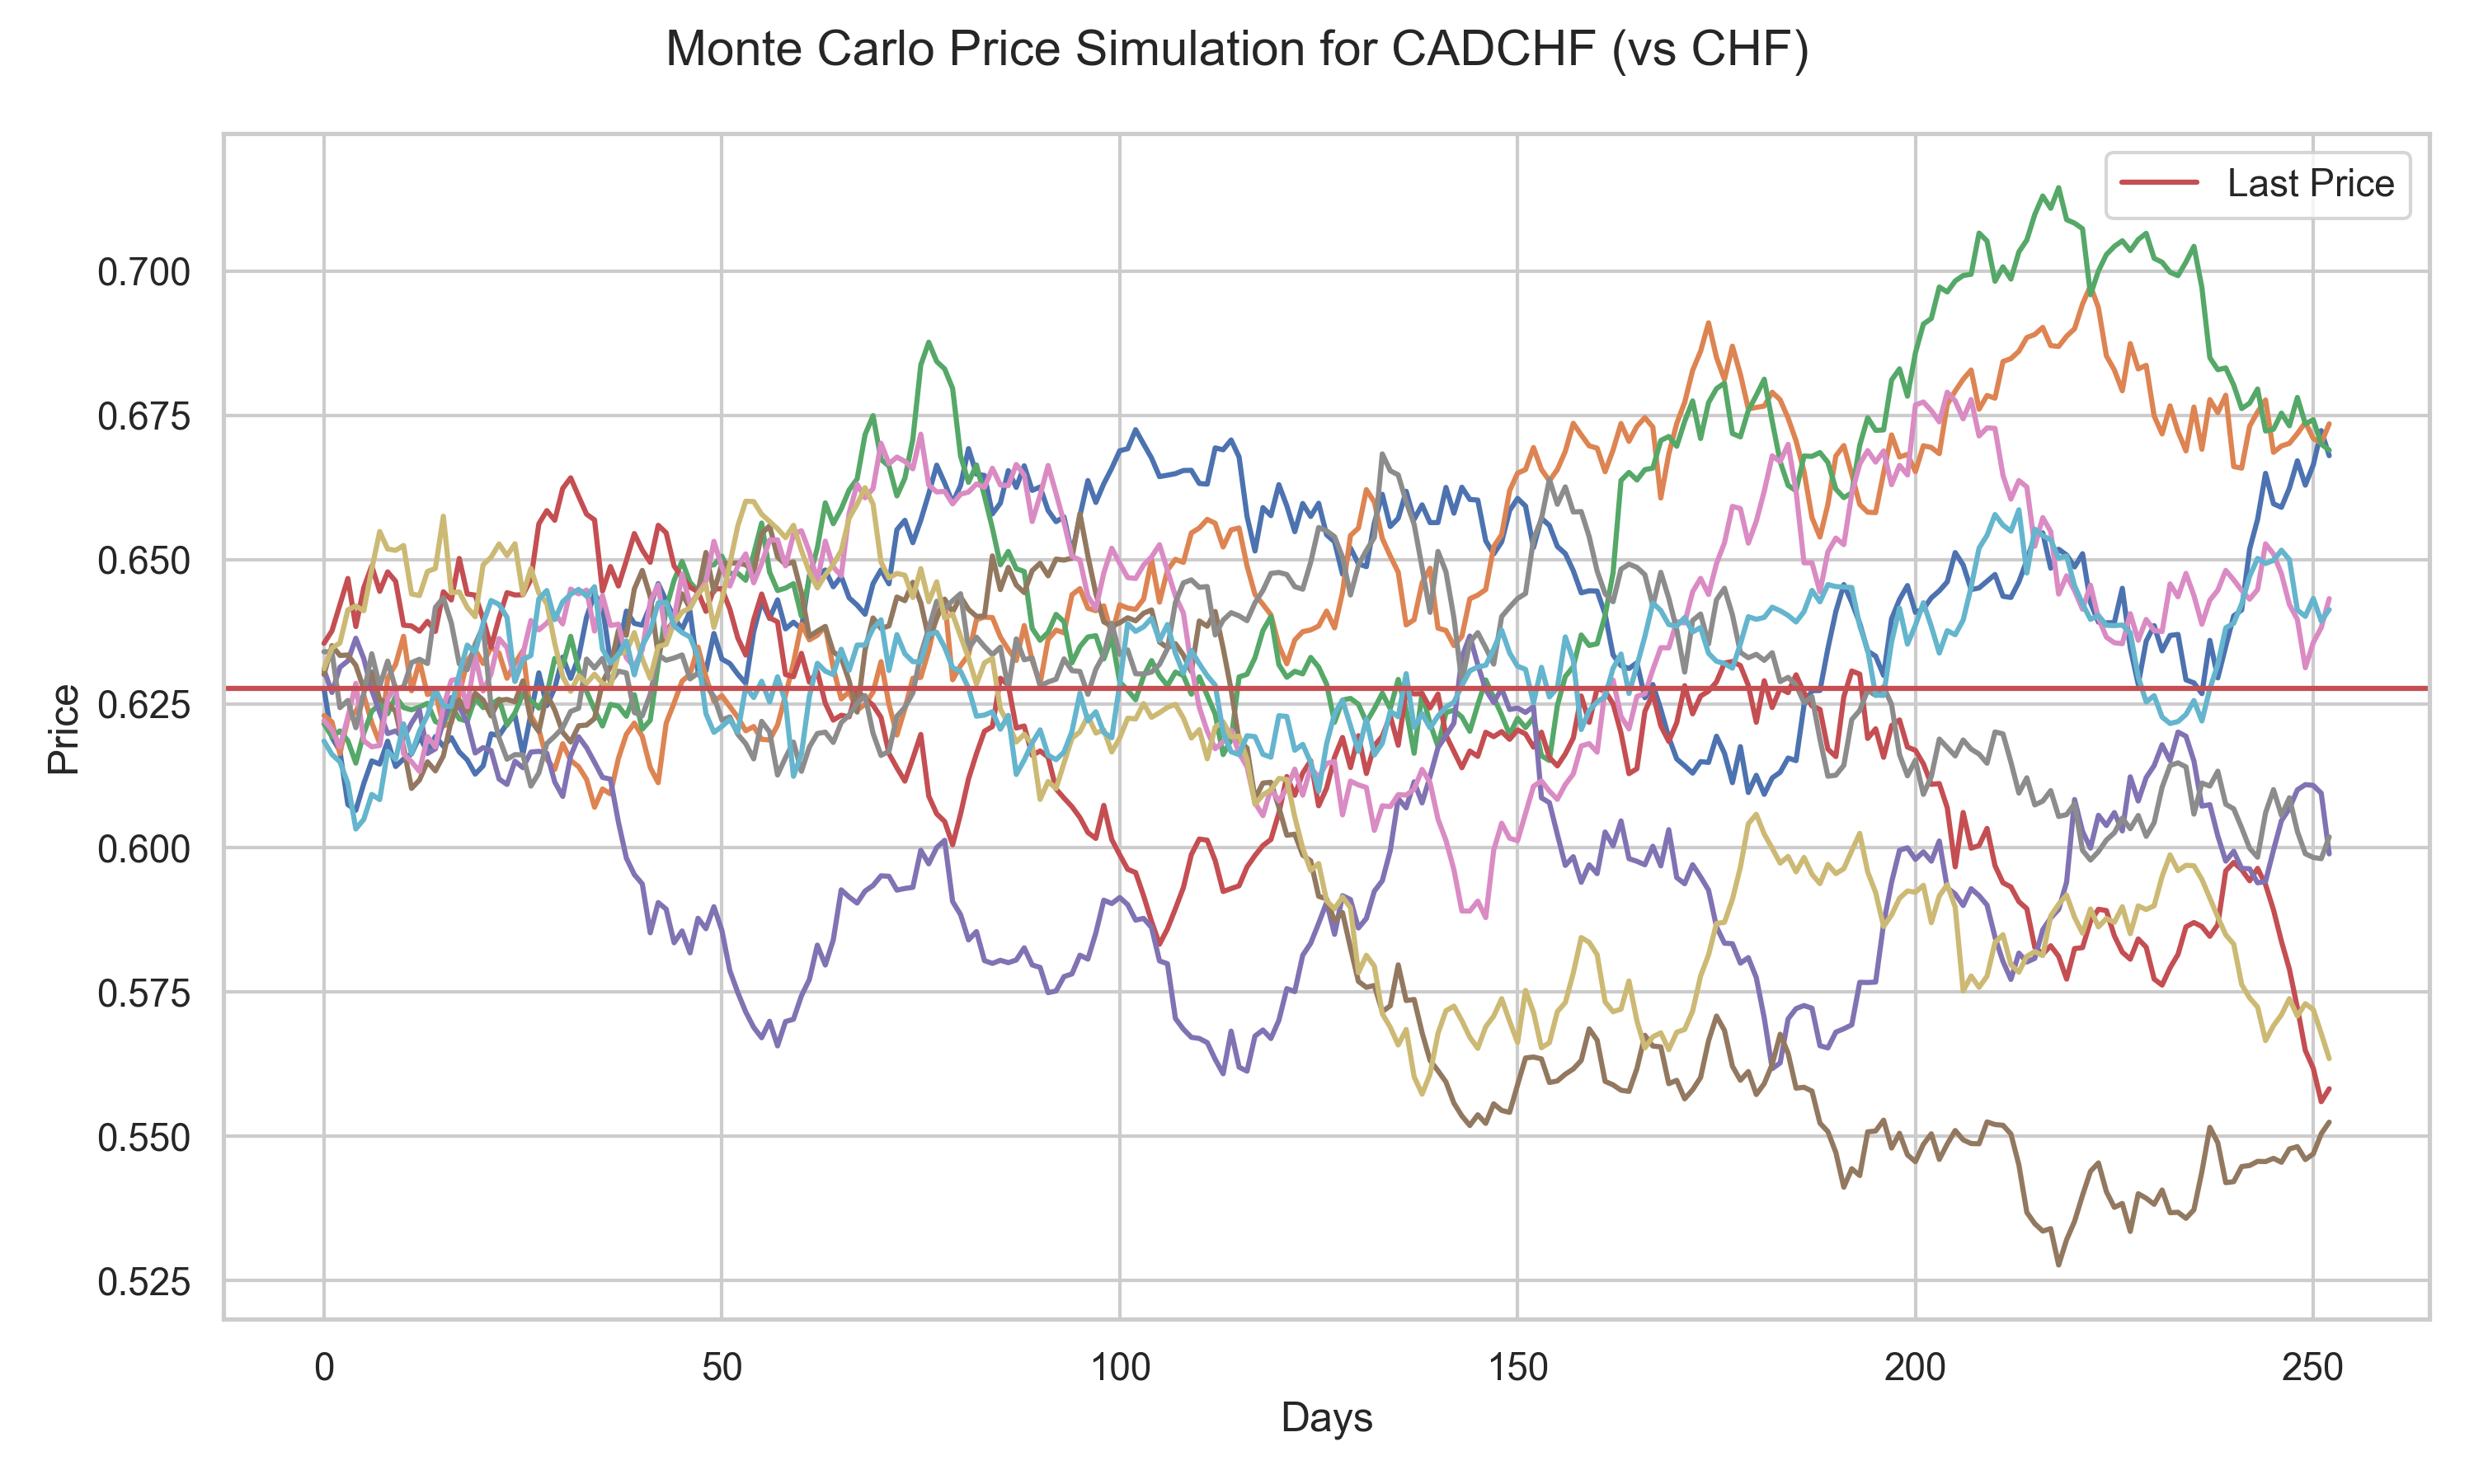
\includegraphics[width=0.48\linewidth]{../../reports/figures/monte_carlo_price_simulation_CADCHF_vs_CHF.png} \label{fig:monte_carlo_price_simulation_CADCHF_vs_CHF}
    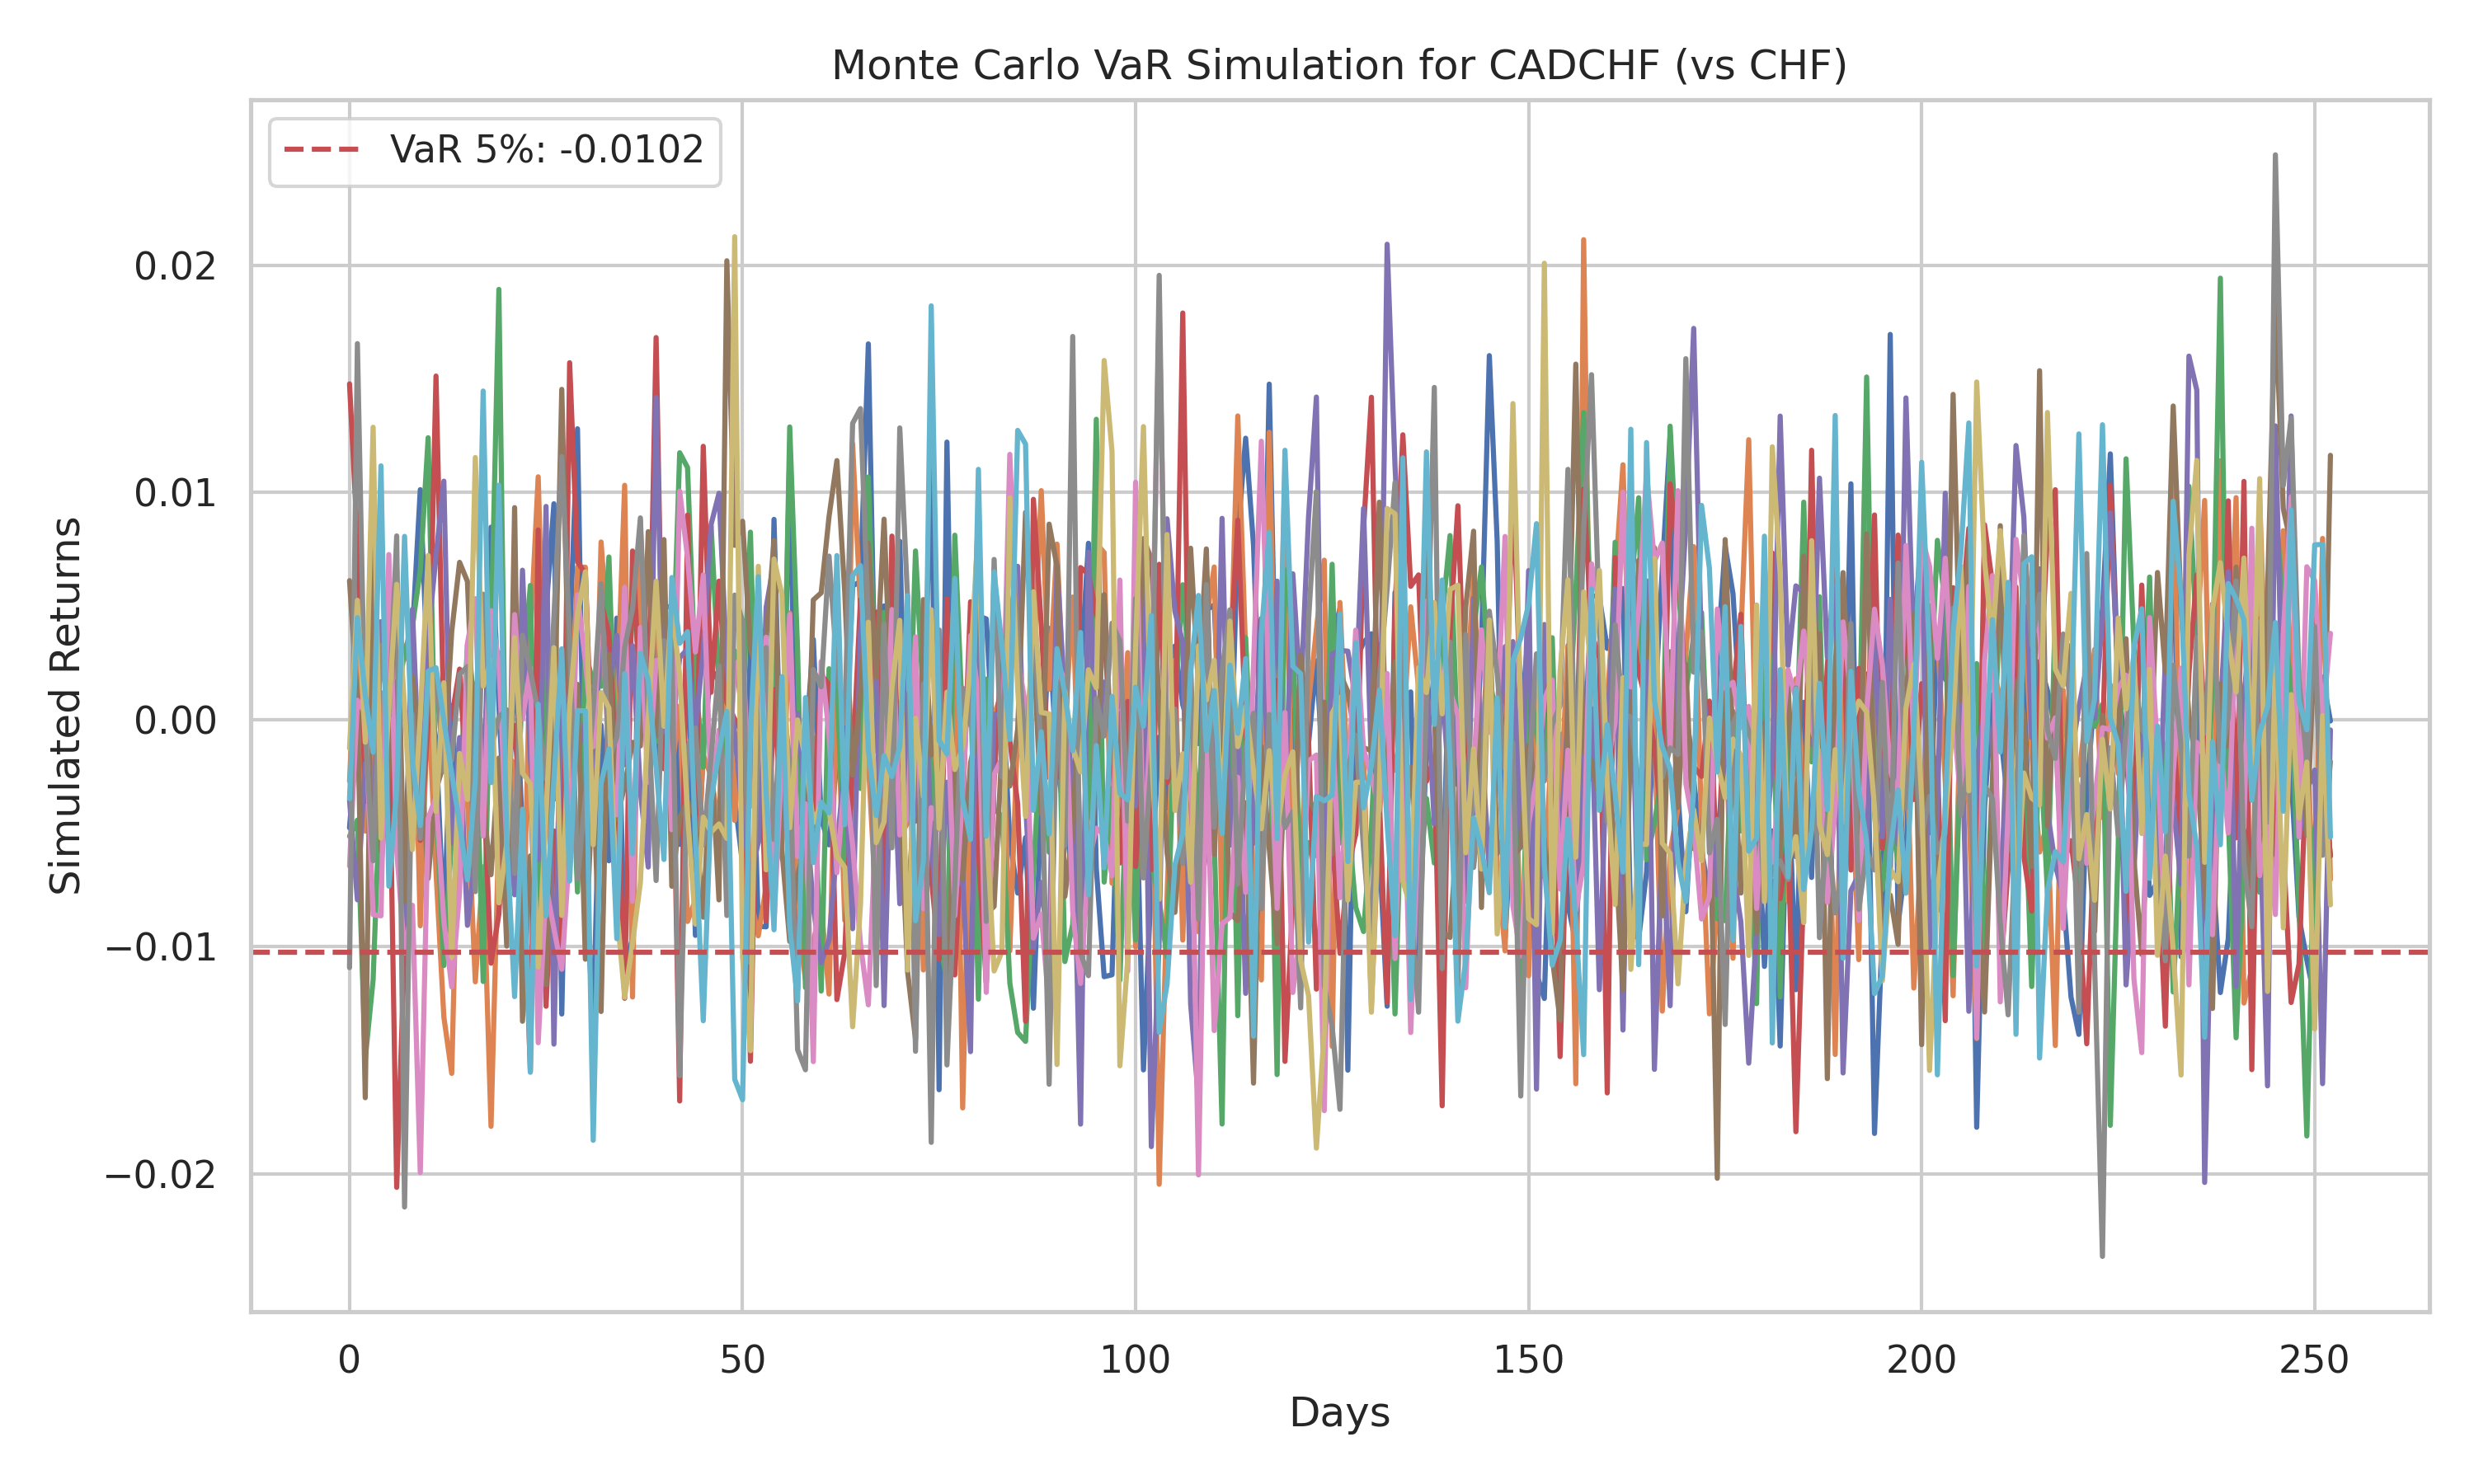
\includegraphics[width=0.48\linewidth]{../../reports/figures/monte_carlo_var_simulation_CADCHF_vs_CHF.png} \label{fig:monte_carlo_var_simulation_CADCHF_vs_CHF}
    \caption{\footnotesize Monte Carlo price siulation (left) and VaR simulation (right) for CAD-CHF.}
\end{figure}

\begin{figure}[H]
    \centering  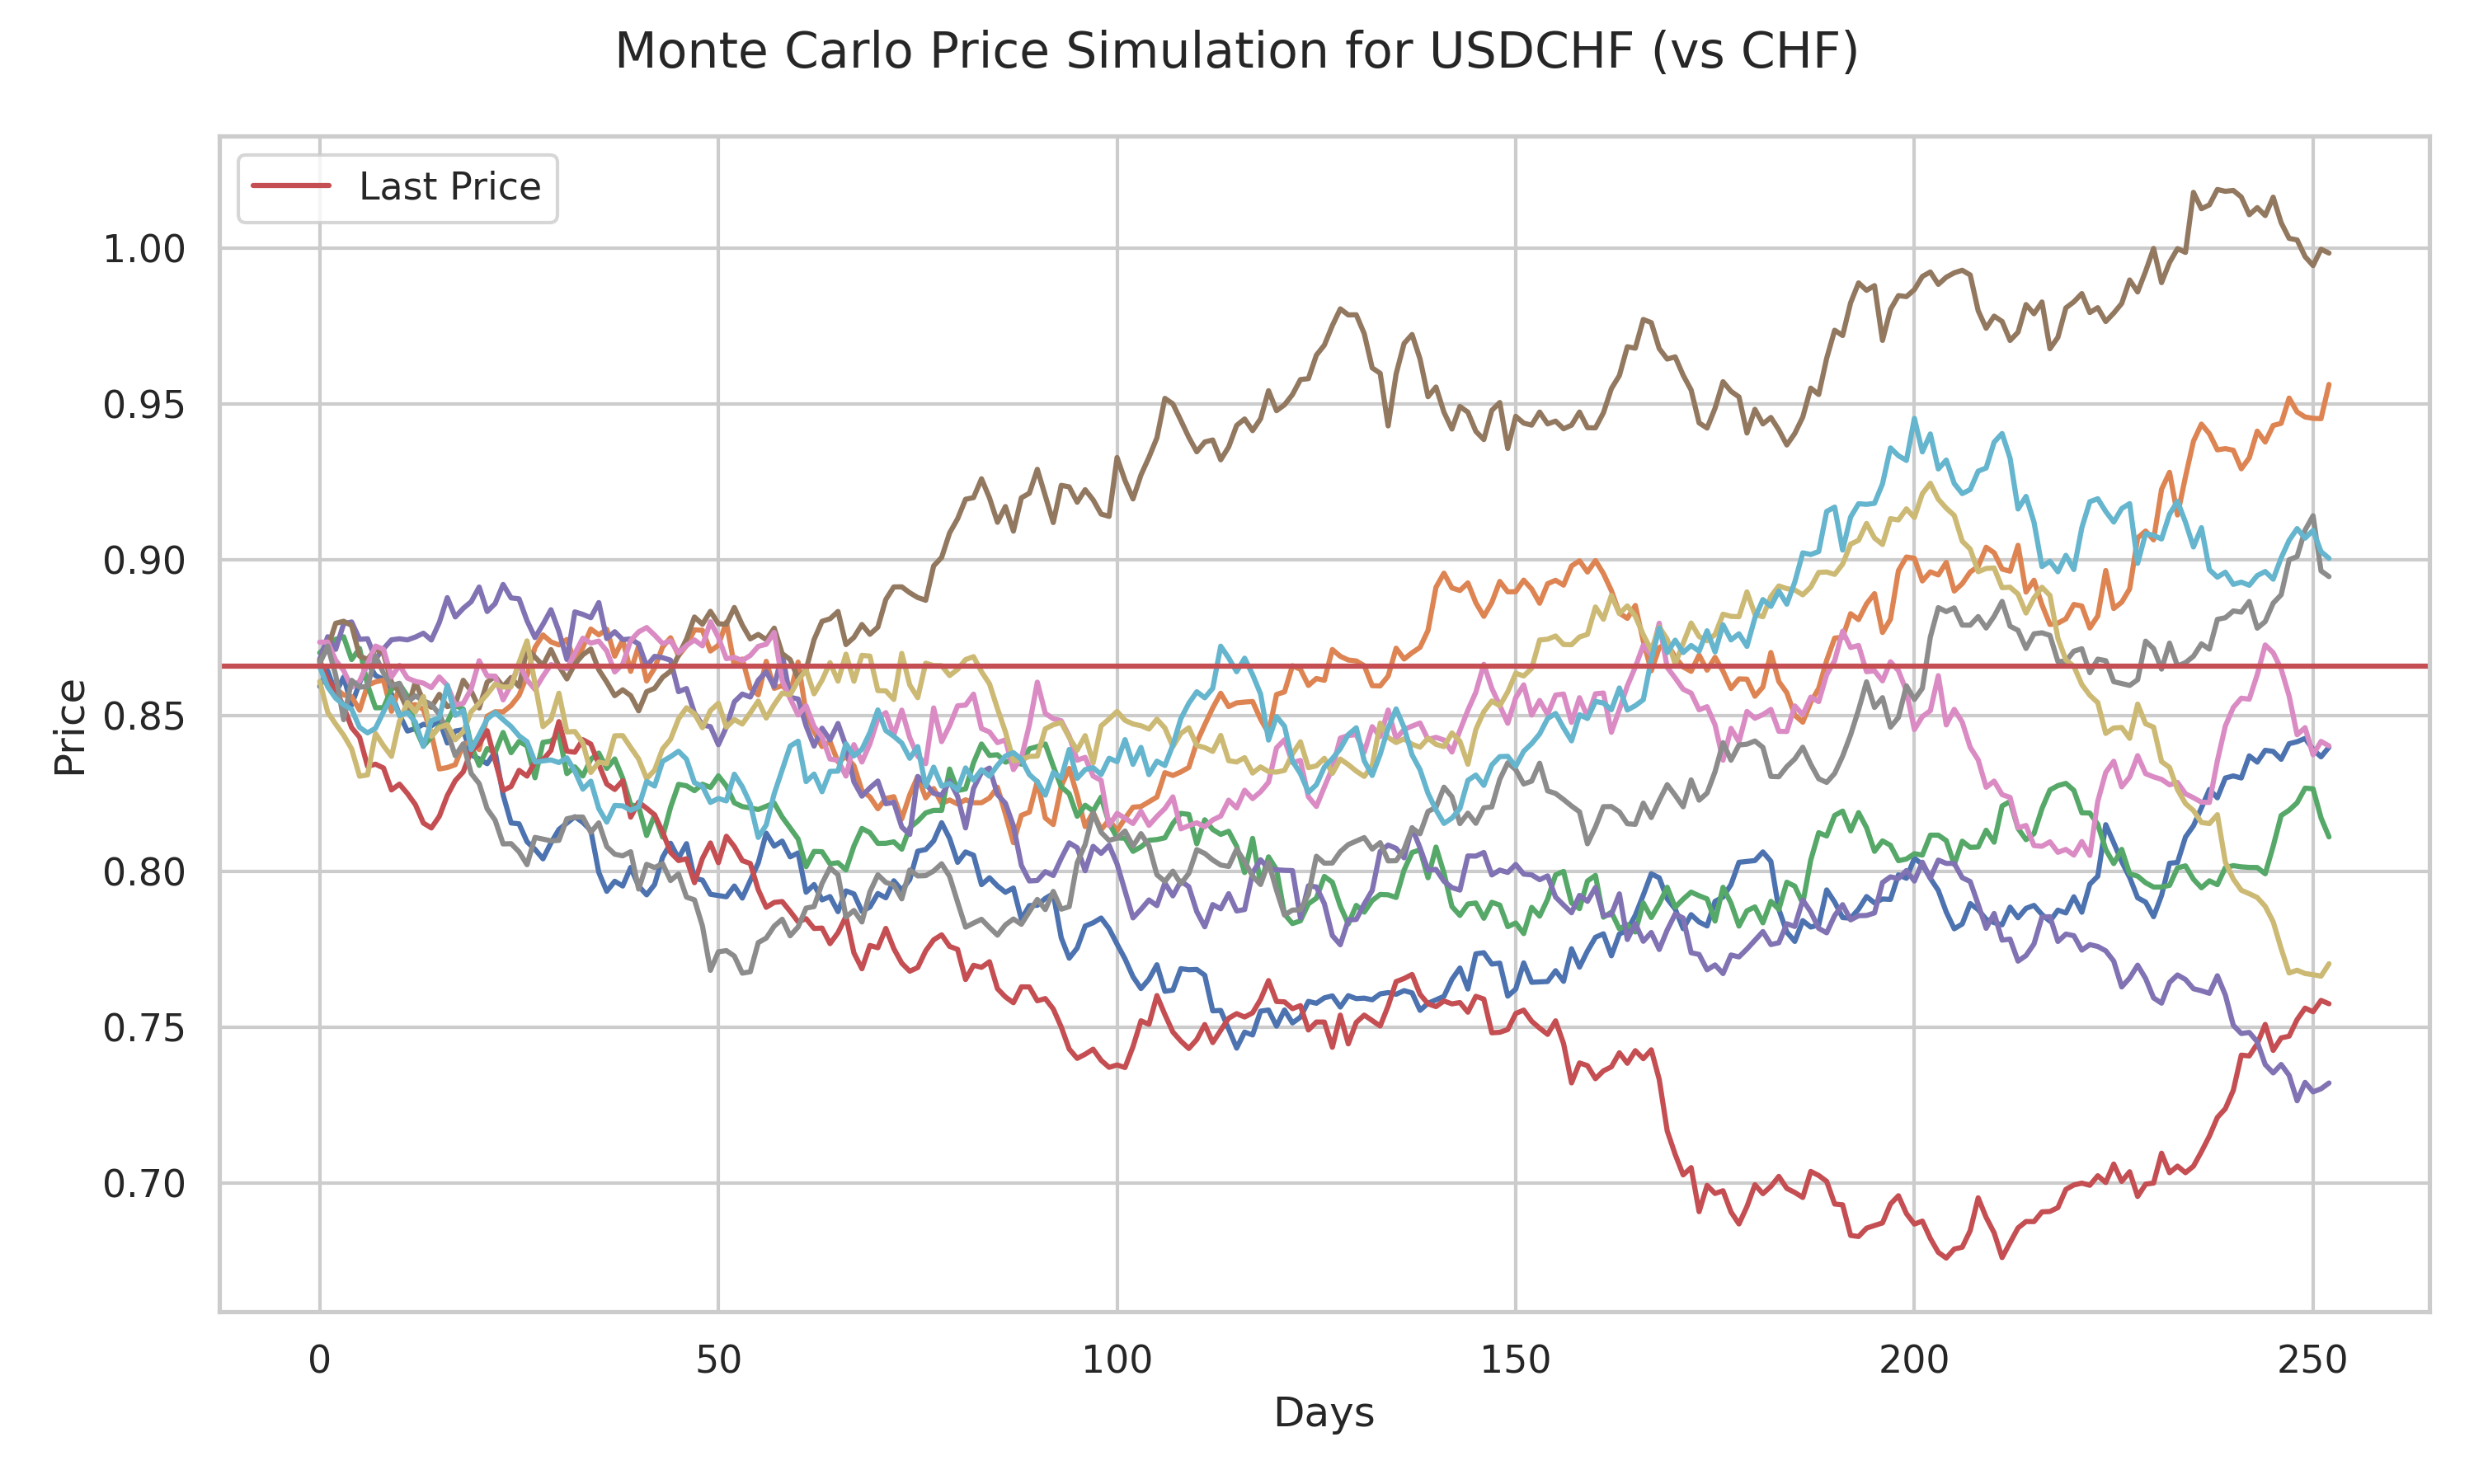
\includegraphics[width=0.48\linewidth]{../../reports/figures/monte_carlo_price_simulation_USDCHF_vs_CHF.png} \label{fig:monte_carlo_price_simulation_USDCHF_vs_CHF}
    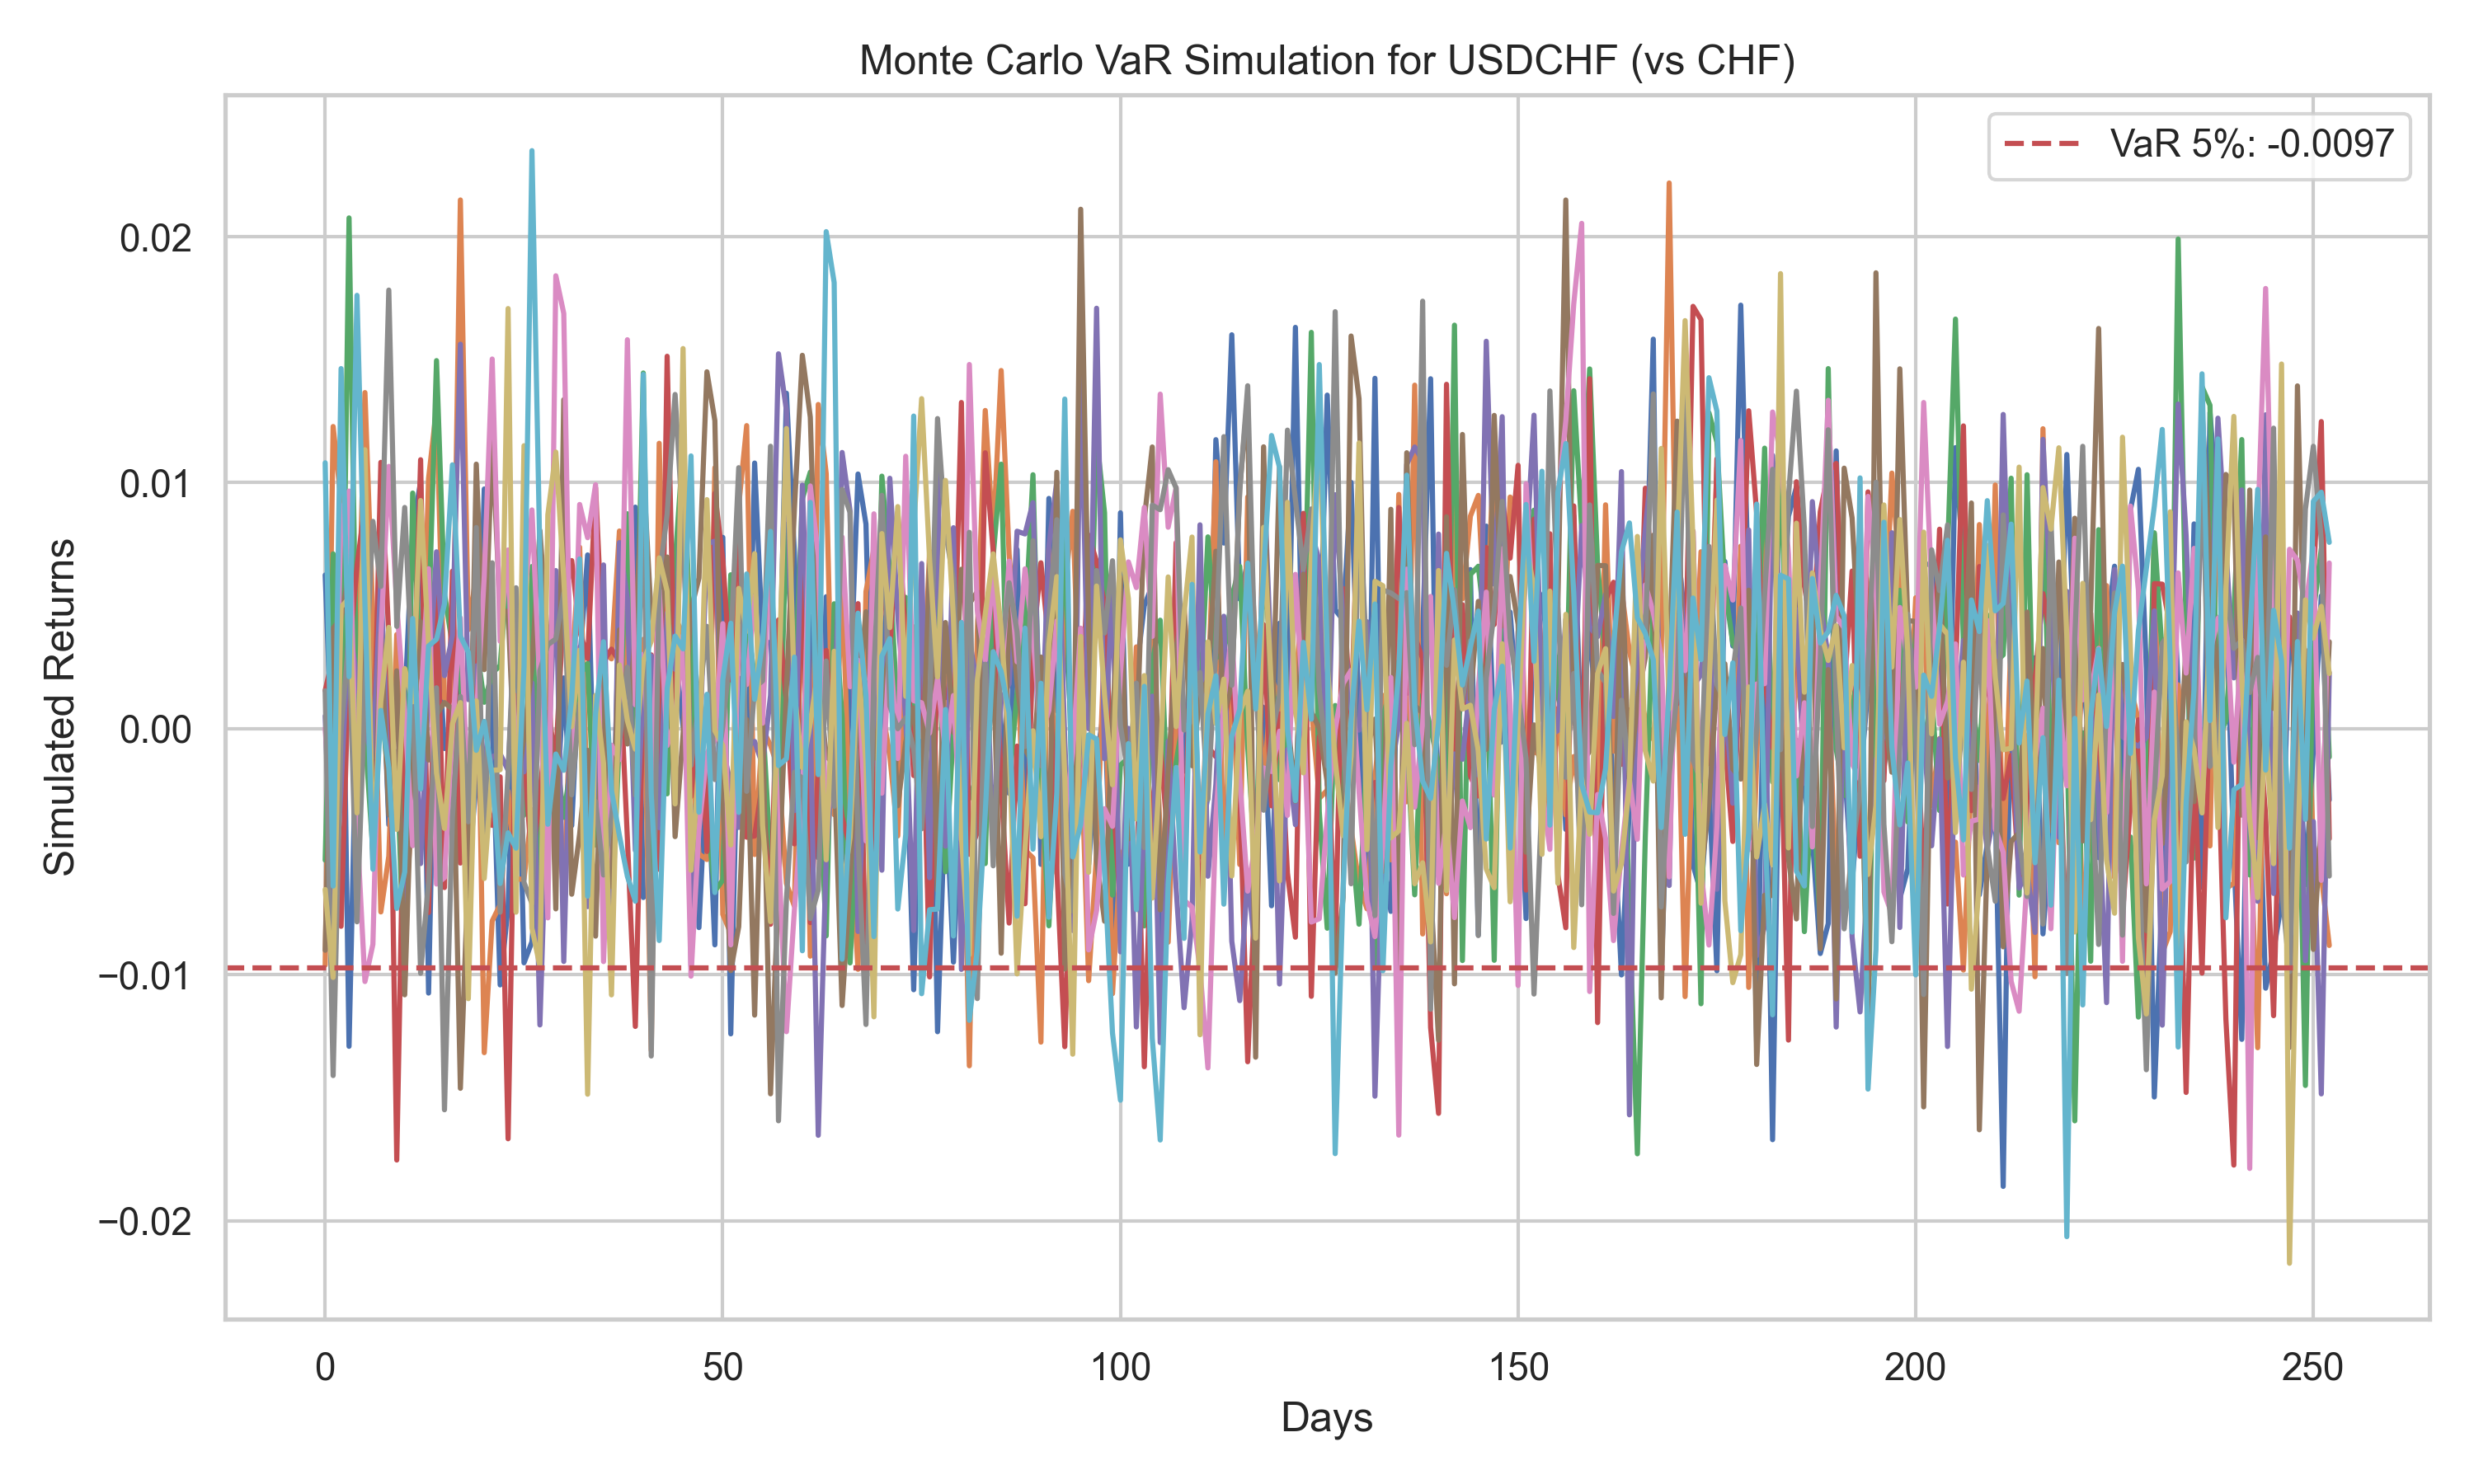
\includegraphics[width=0.48\linewidth]{../../reports/figures/monte_carlo_var_simulation_USDCHF_vs_CHF.png} \label{fig:monte_carlo_var_simulation_USDCHF_vs_CHF}
    \caption{\footnotesize Monte Carlo price siulation (left) and VaR simulation (right) for USD-CHF.}
\end{figure}

\begin{figure}[H]
    \centering  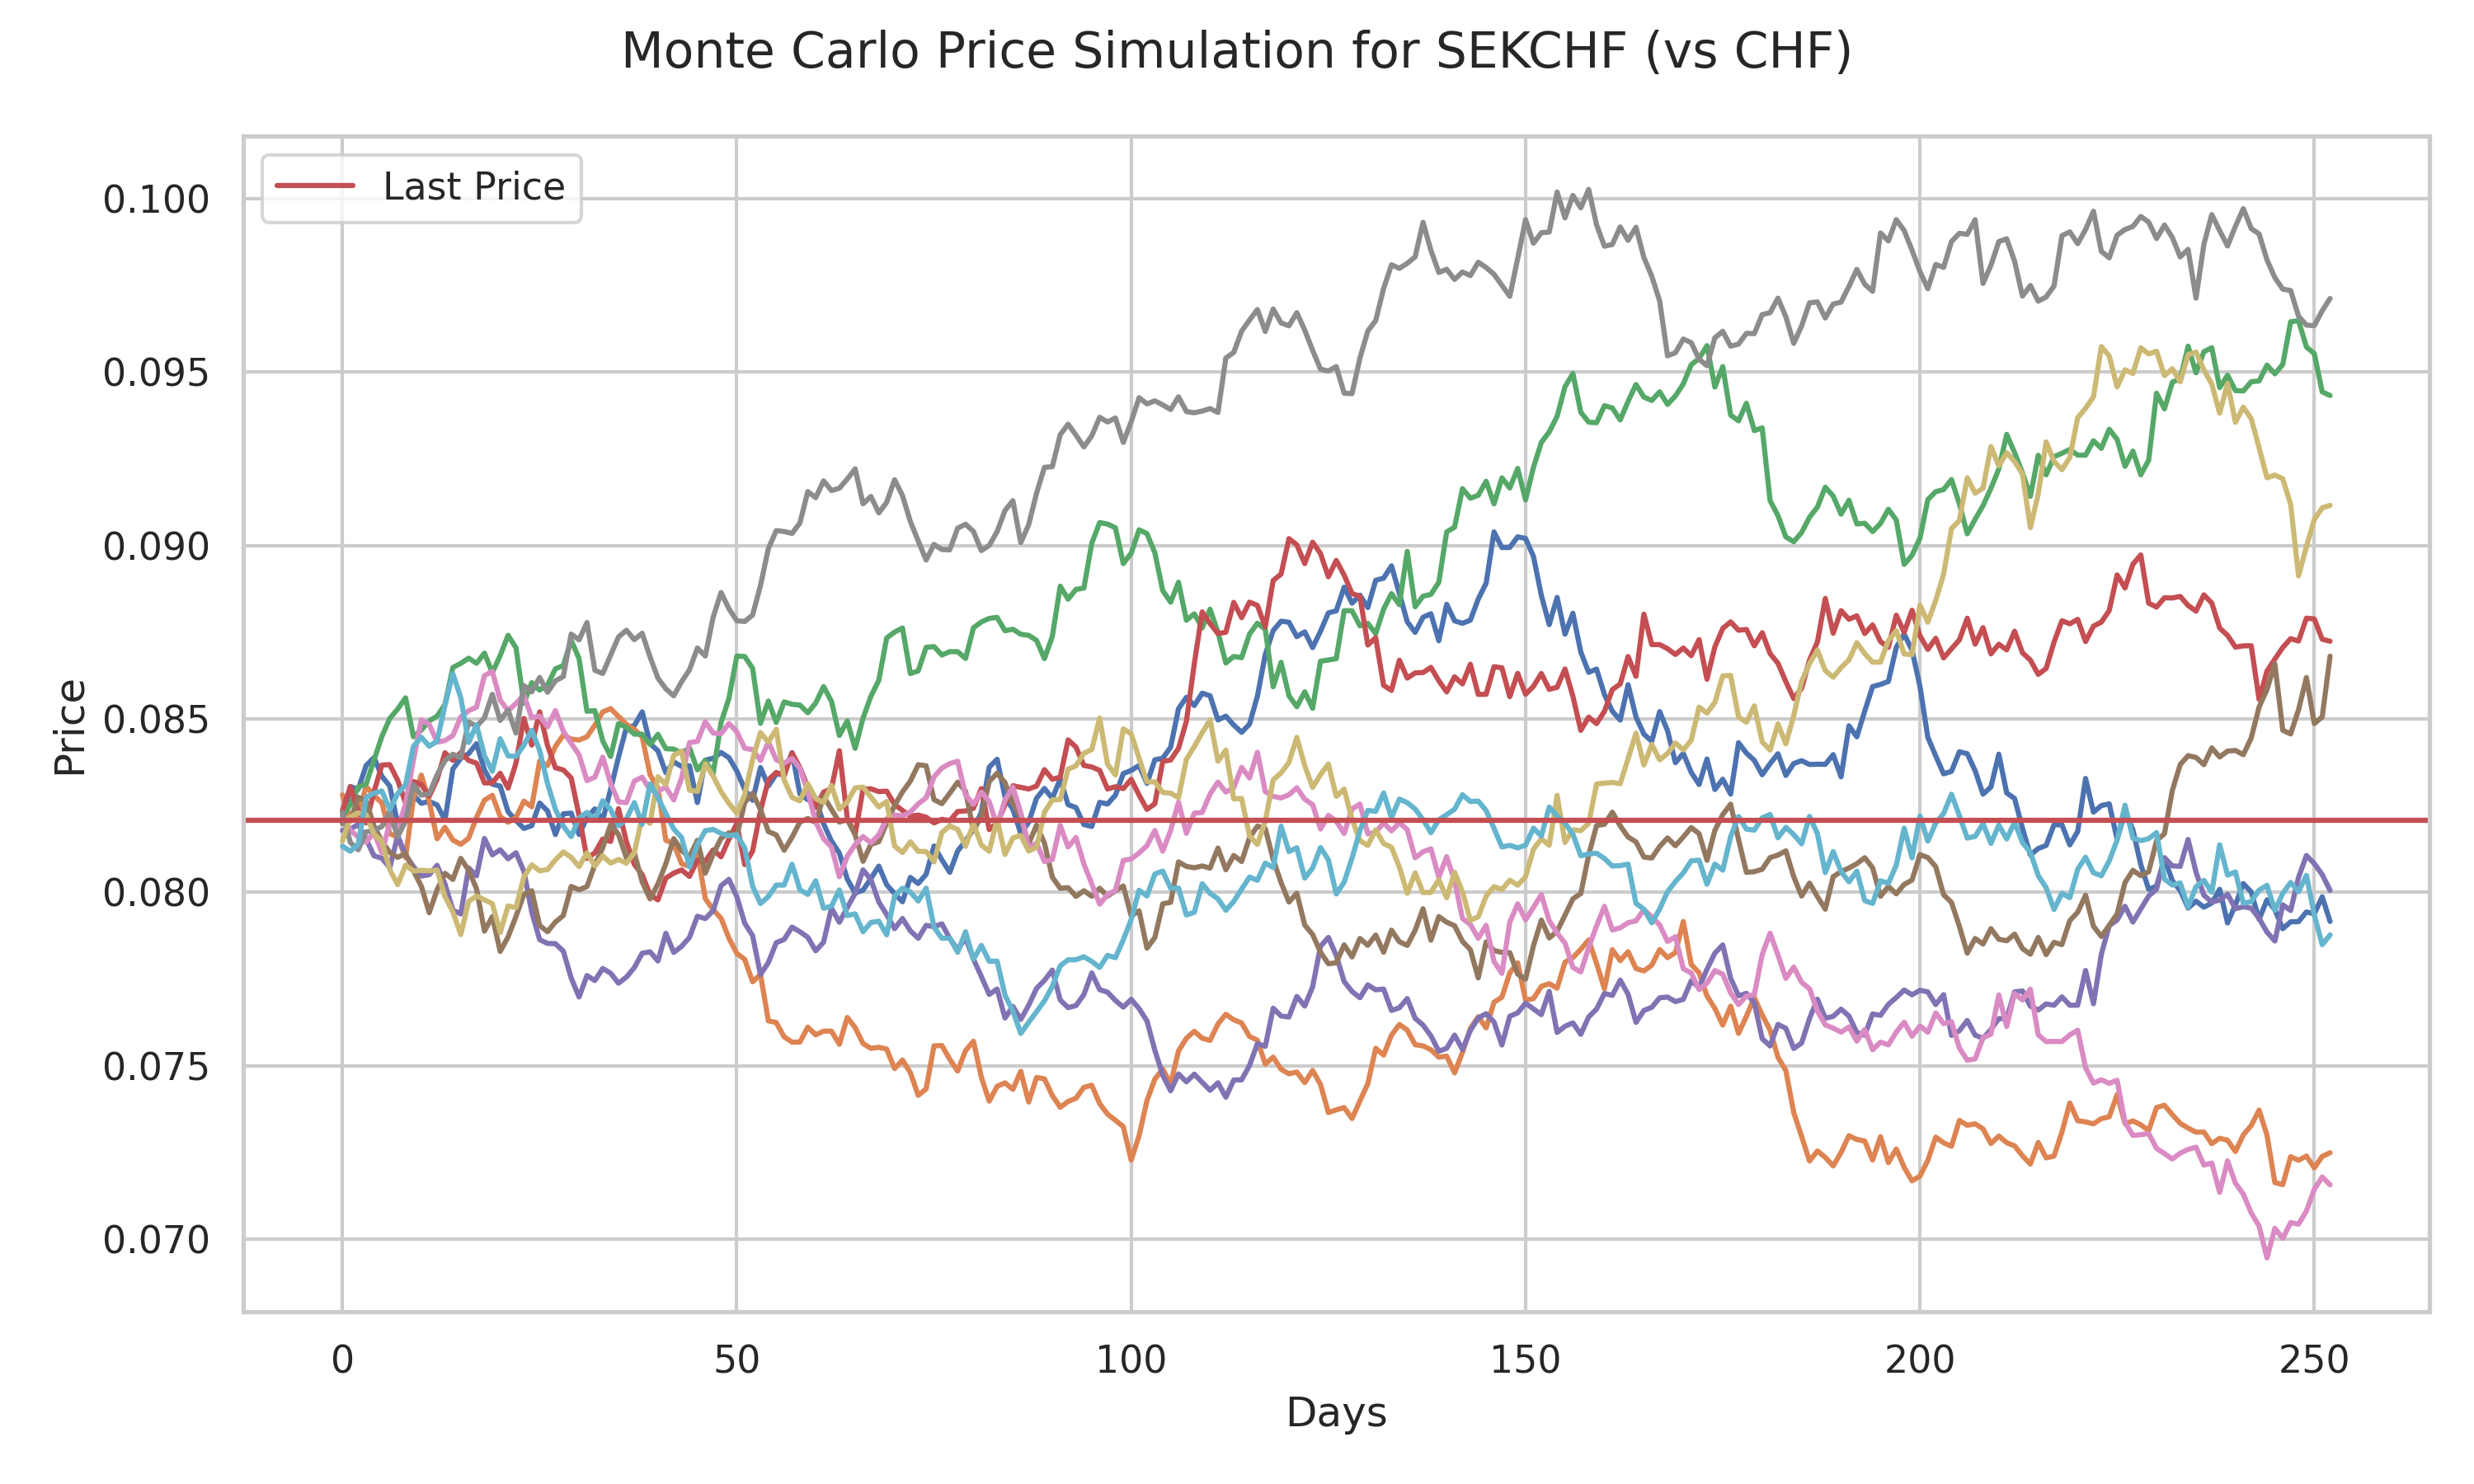
\includegraphics[width=0.48\linewidth]{../../reports/figures/monte_carlo_price_simulation_SEKCHF_vs_CHF.png} \label{fig:monte_carlo_price_simulation_SEKCHF_vs_CHF}
    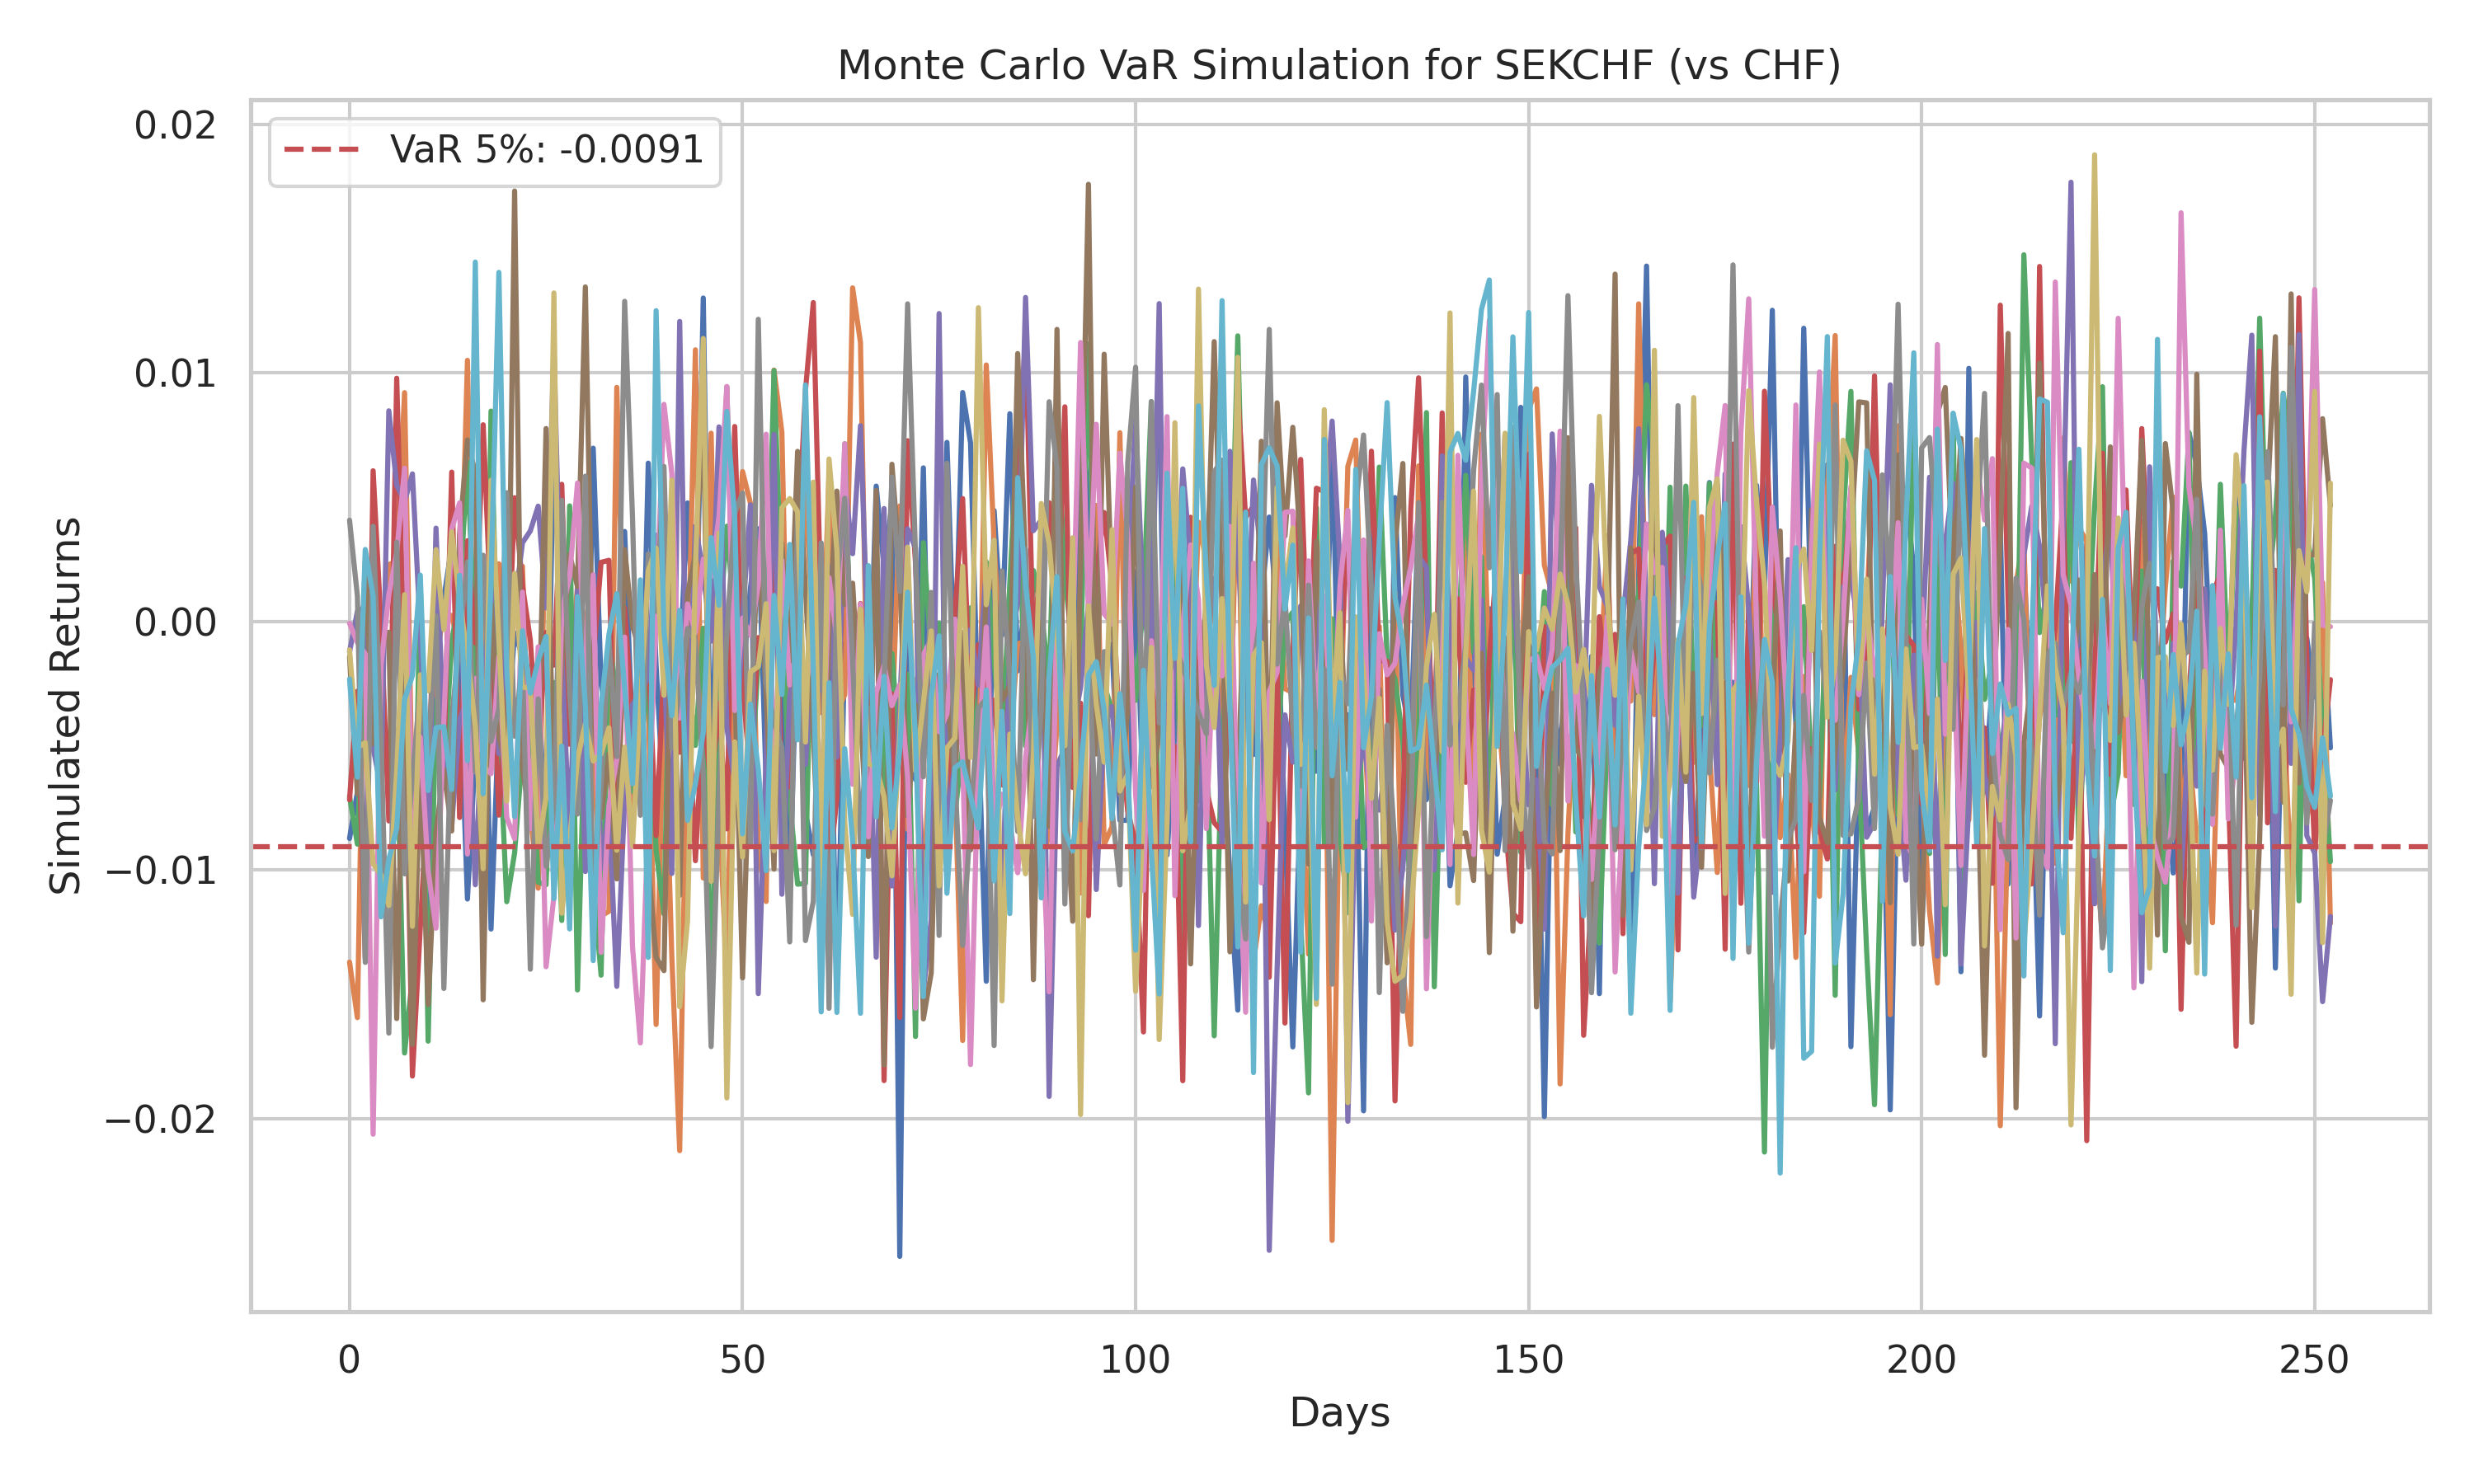
\includegraphics[width=0.48\linewidth]{../../reports/figures/monte_carlo_var_simulation_SEKCHF_vs_CHF.png} \label{fig:monte_carlo_var_simulation_SEKCHF_vs_CHF}
    \caption{\footnotesize Monte Carlo price siulation (left) and VaR simulation (right) for SEK-CHF.}
\end{figure}

\begin{figure}[H]
    \centering  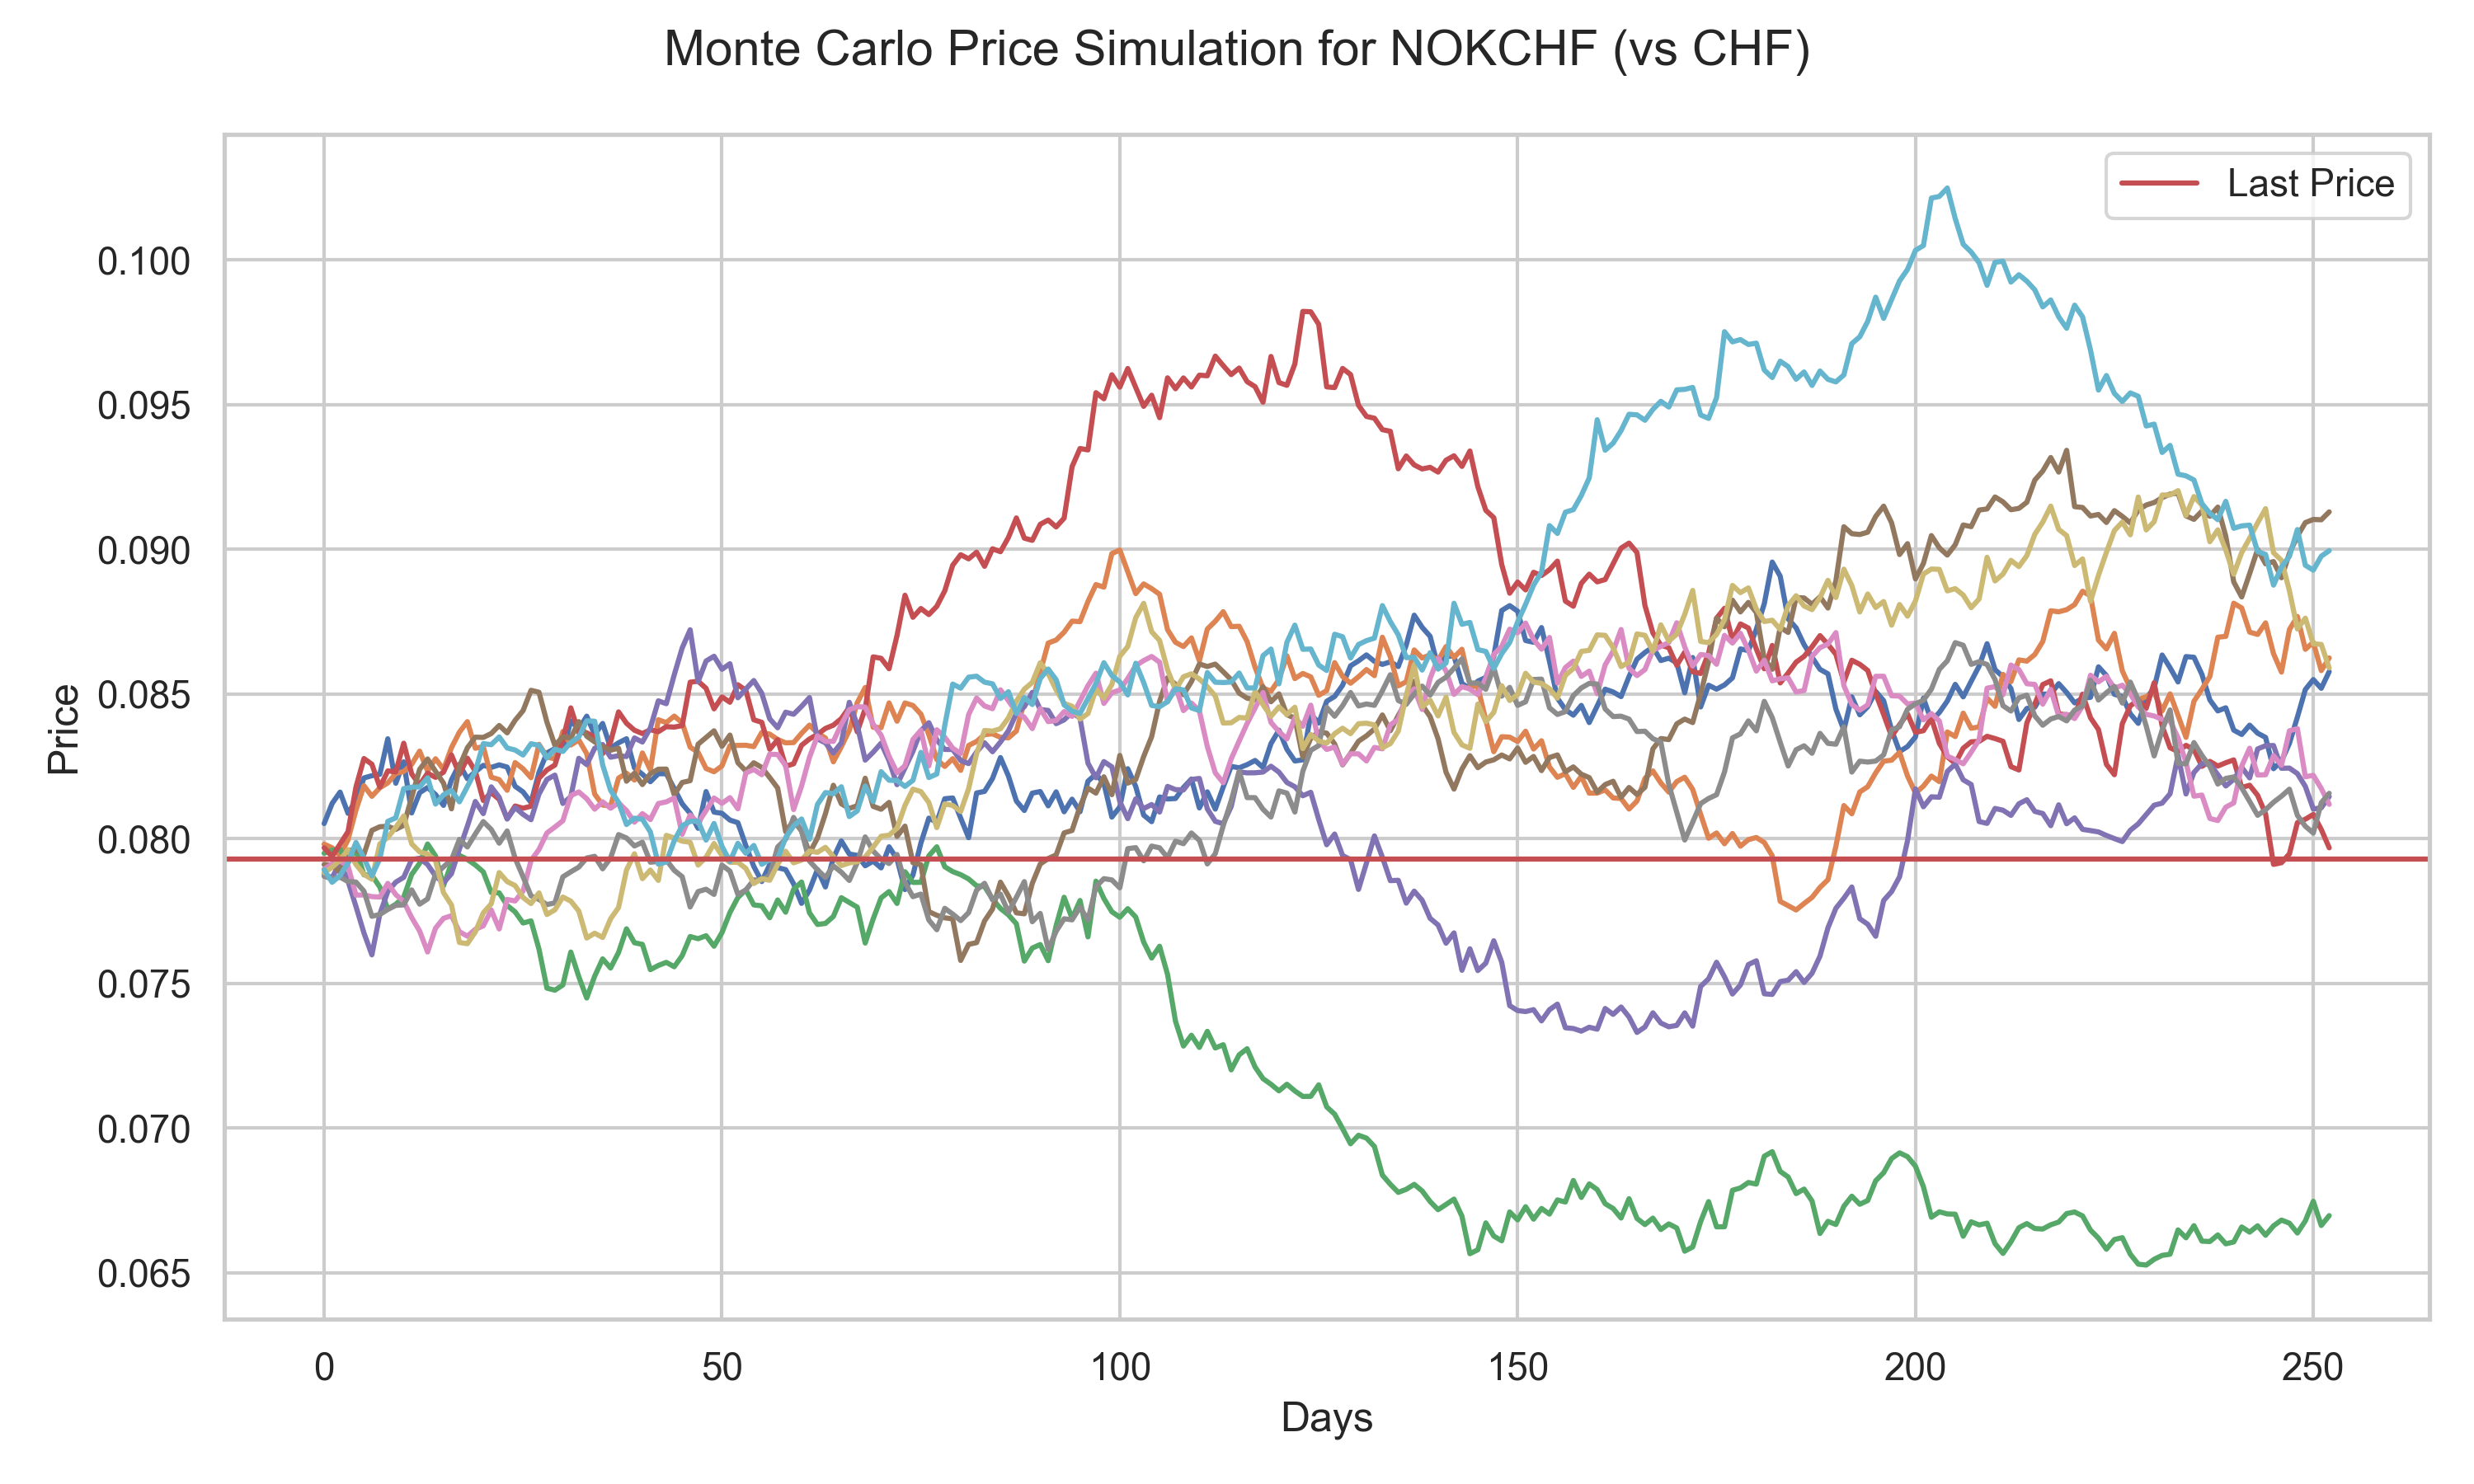
\includegraphics[width=0.48\linewidth]{../../reports/figures/monte_carlo_price_simulation_NOKCHF_vs_CHF.png} \label{fig:monte_carlo_price_simulation_NOKCHF_vs_CHF}
    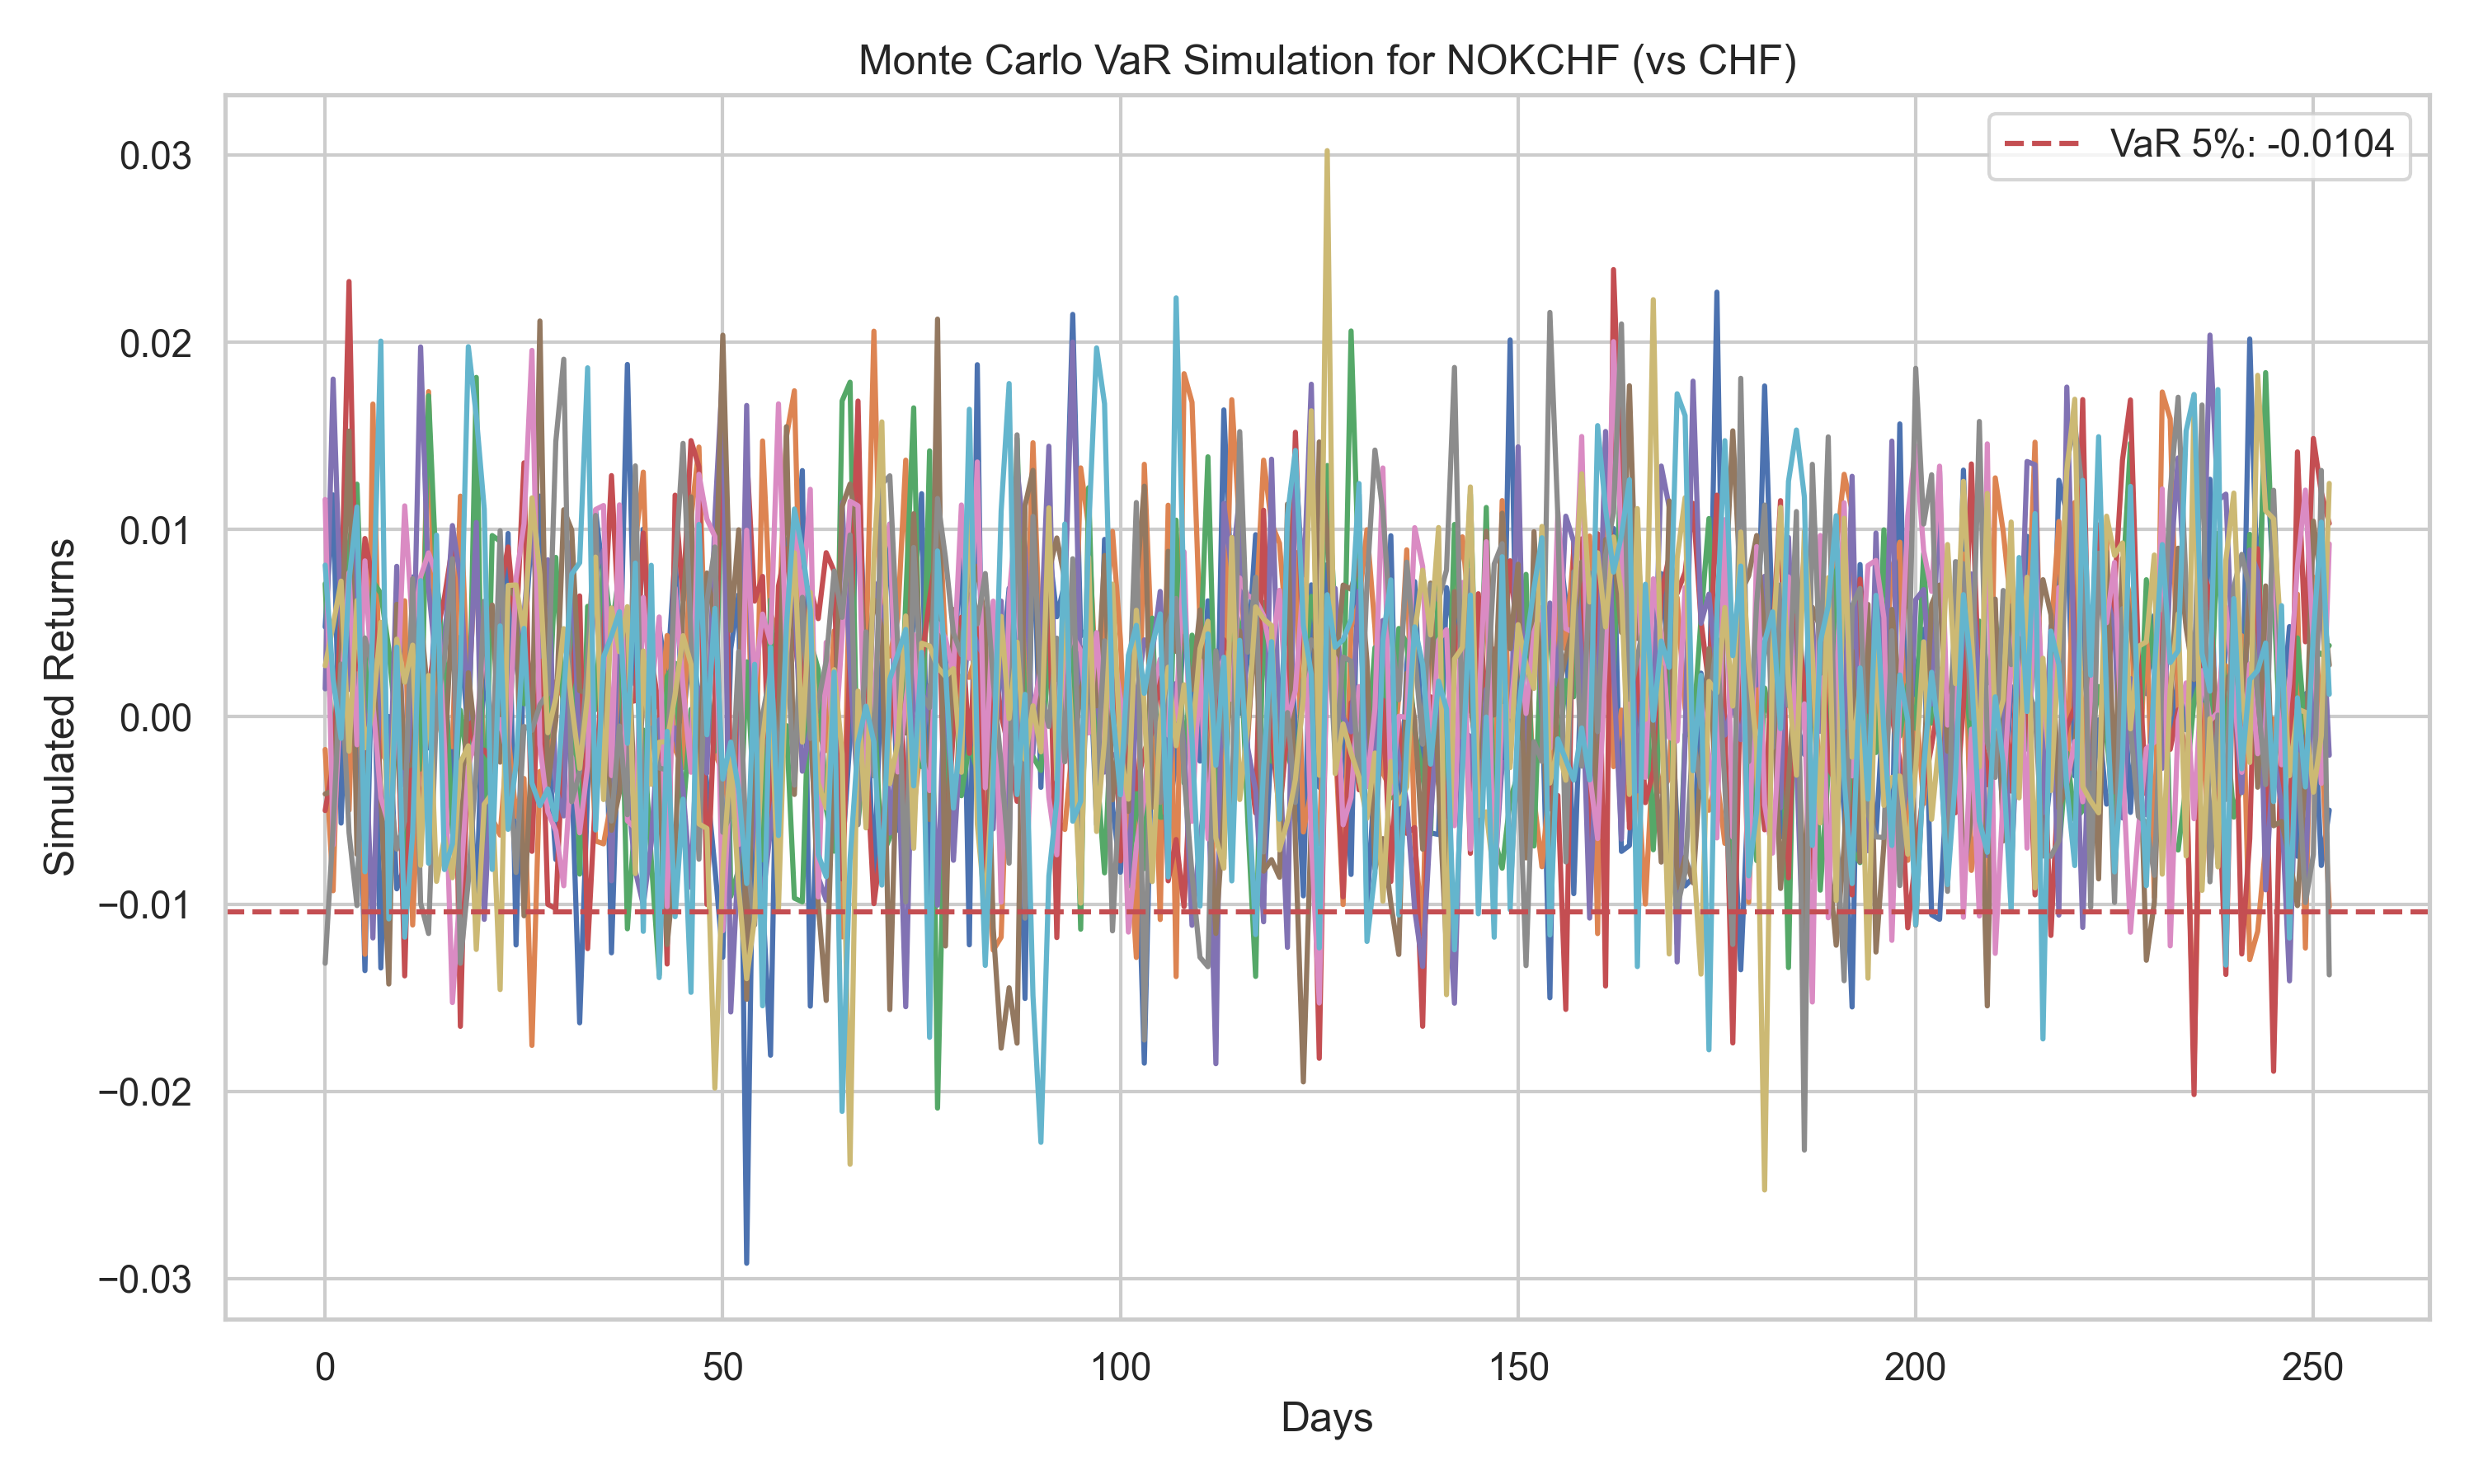
\includegraphics[width=0.48\linewidth]{../../reports/figures/monte_carlo_var_simulation_NOKCHF_vs_CHF.png} \label{fig:monte_carlo_var_simulation_NOKCHF_vs_CHF}
    \caption{\footnotesize Monte Carlo price siulation (left) and VaR simulation (right) for NOK-CHF.}
\end{figure}

\begin{figure}[H]
    \centering  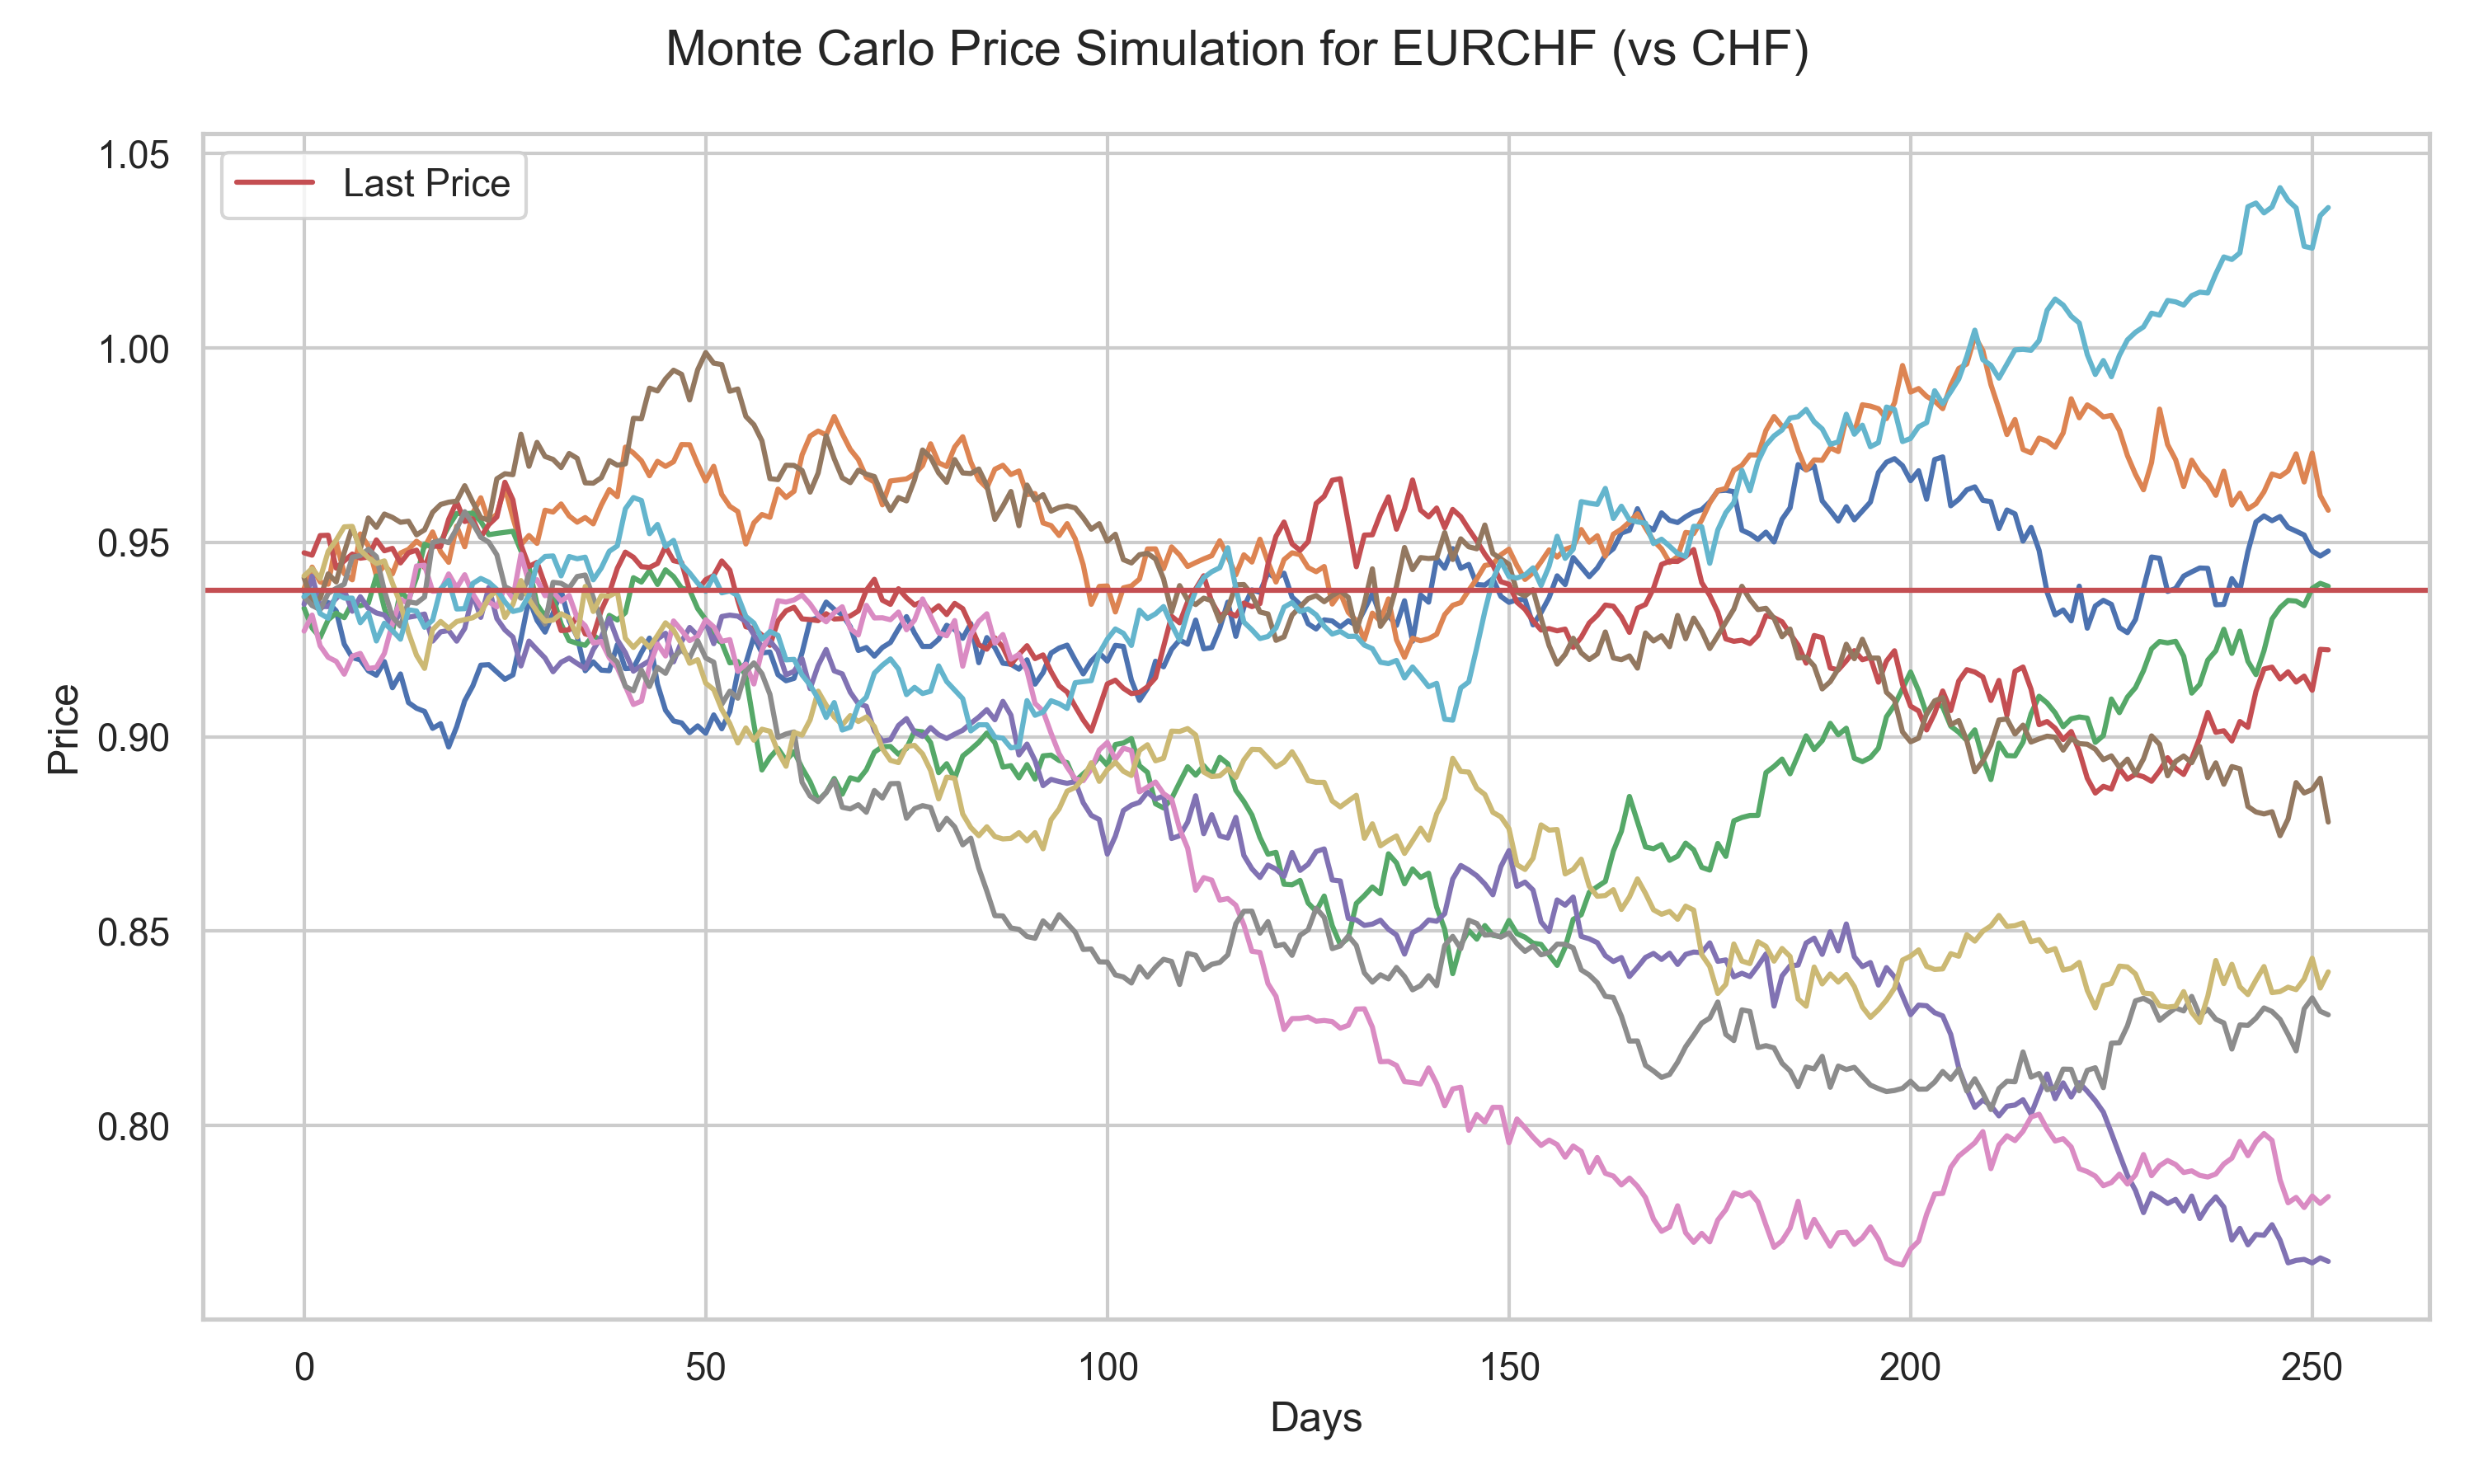
\includegraphics[width=0.48\linewidth]{../../reports/figures/monte_carlo_price_simulation_EURCHF_vs_CHF.png} \label{fig:monte_carlo_price_simulation_EURCHF_vs_CHF}
    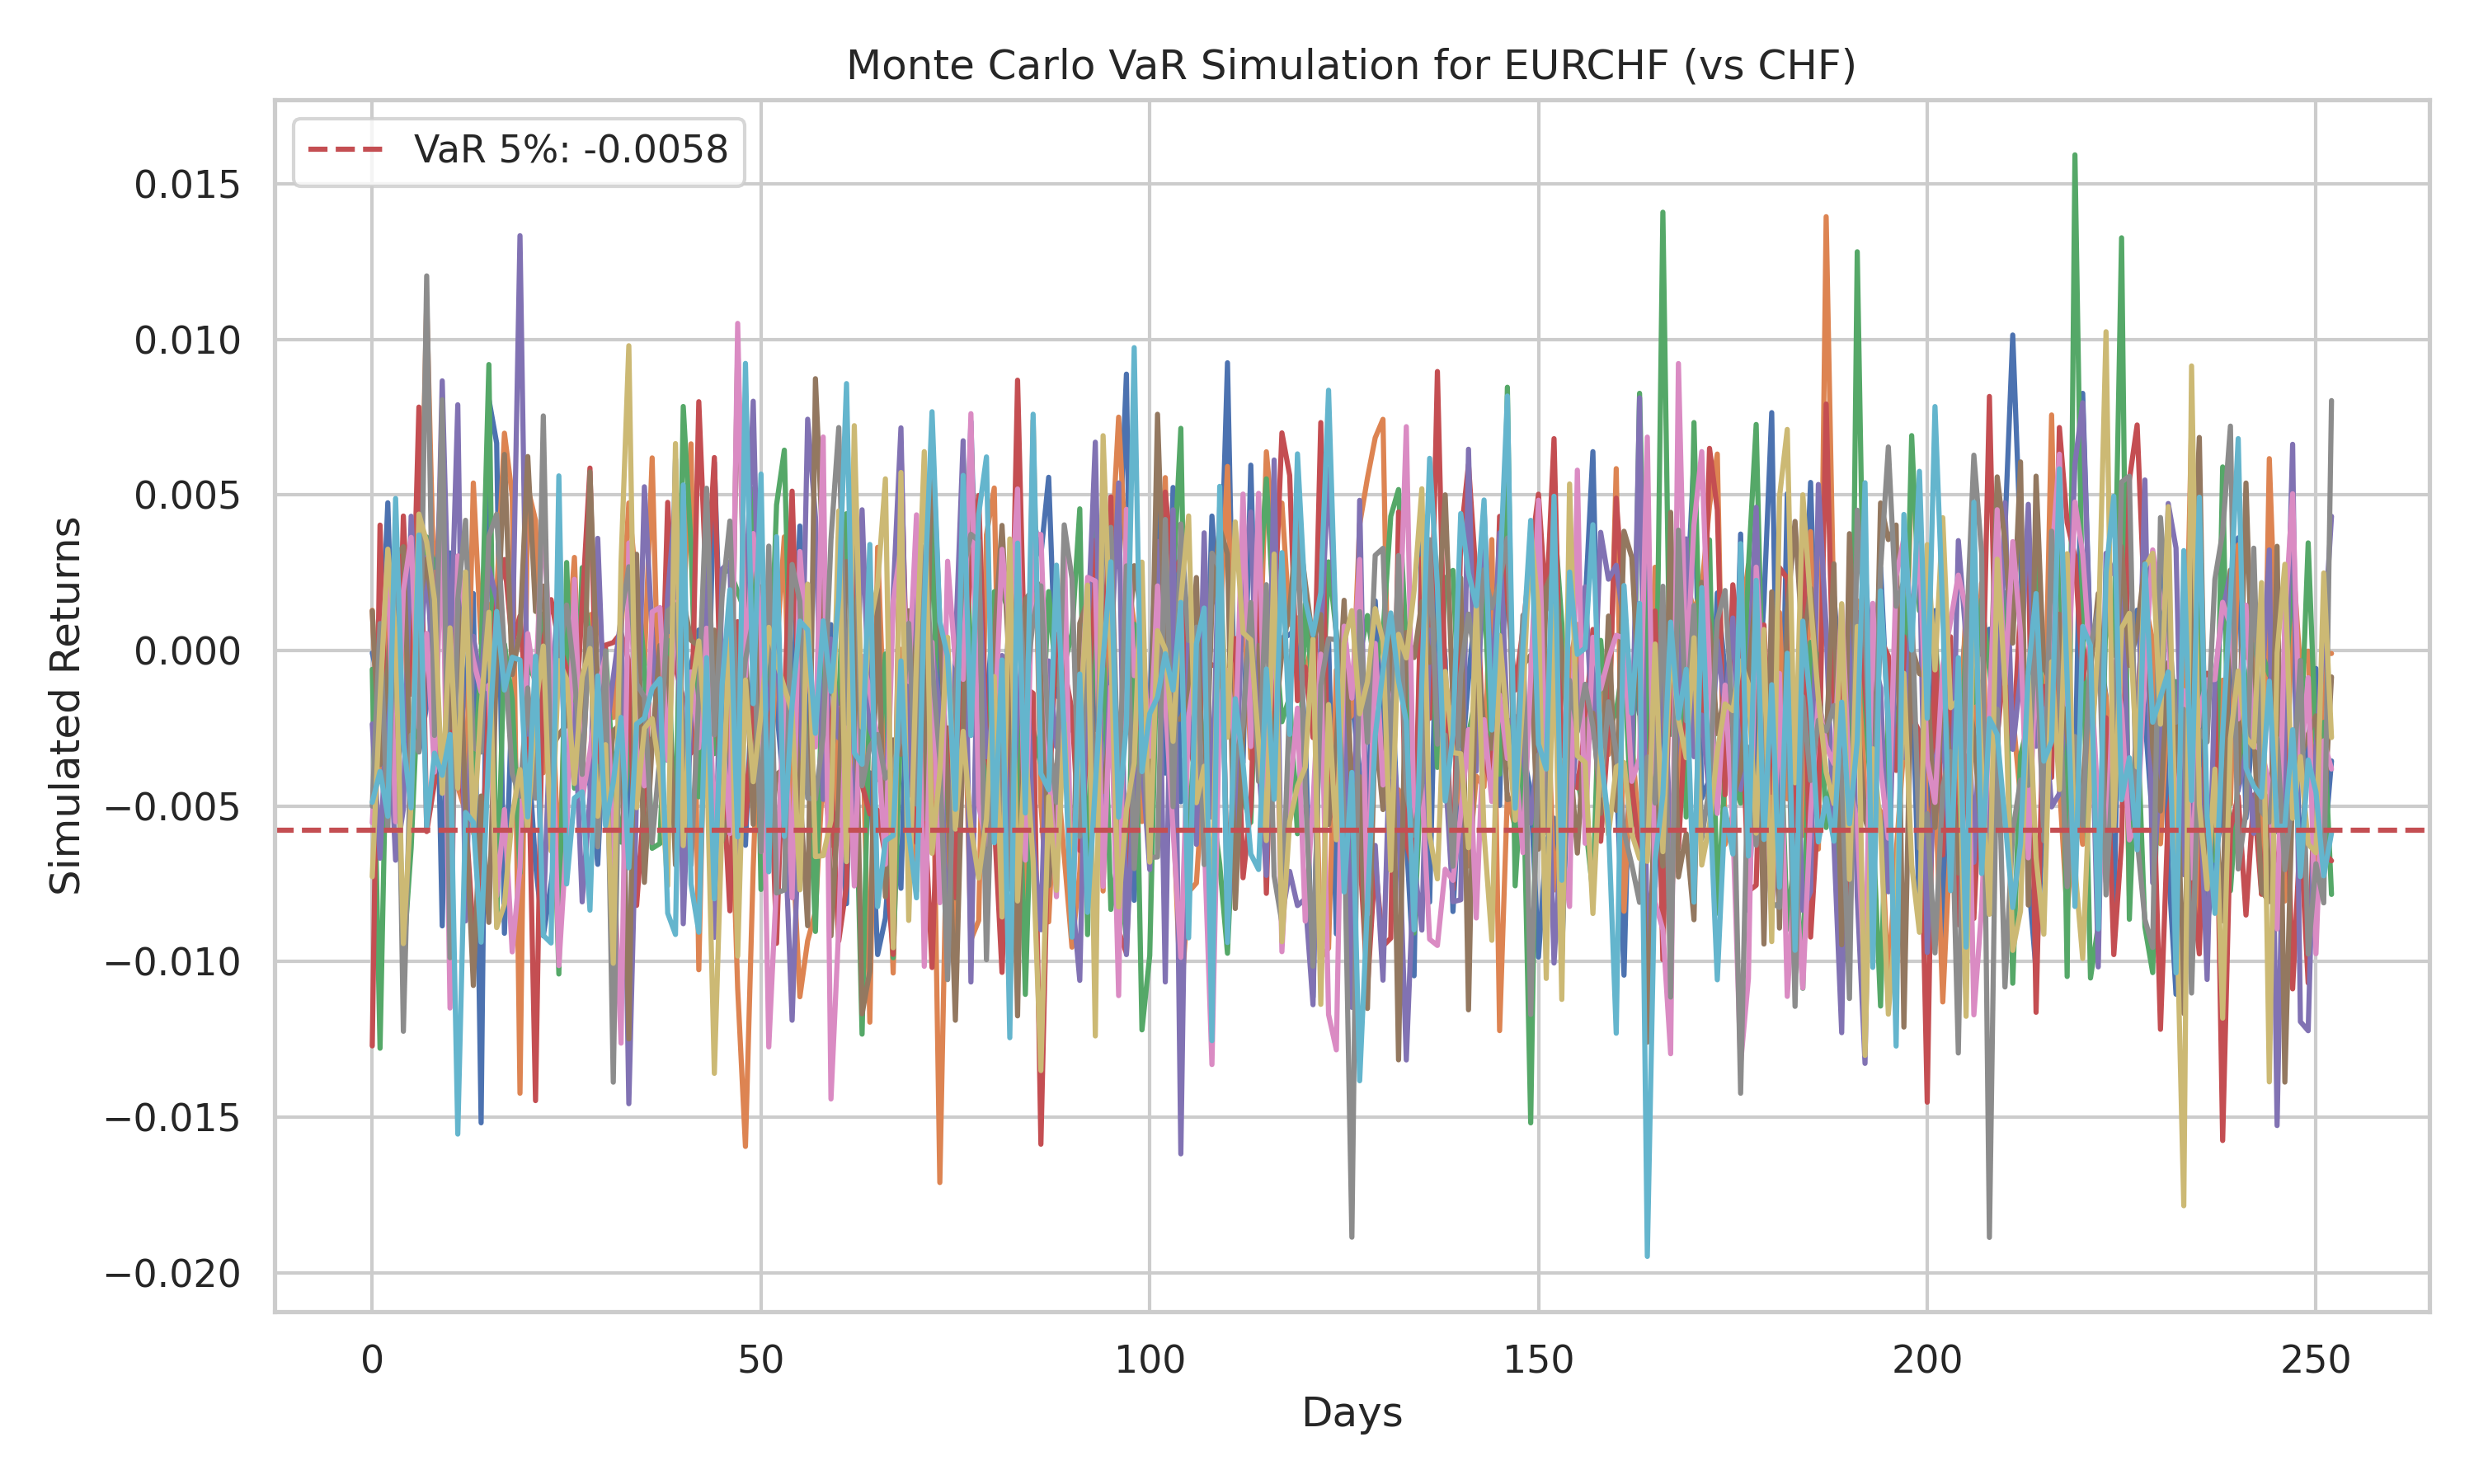
\includegraphics[width=0.48\linewidth]{../../reports/figures/monte_carlo_var_simulation_EURCHF_vs_CHF.png} \label{fig:monte_carlo_var_simulation_EURCHF_vs_CHF}
    \caption{\footnotesize Monte Carlo price siulation (left) and VaR simulation (right) for EUR-CHF.}
\end{figure}

\begin{figure}[H]
    \centering  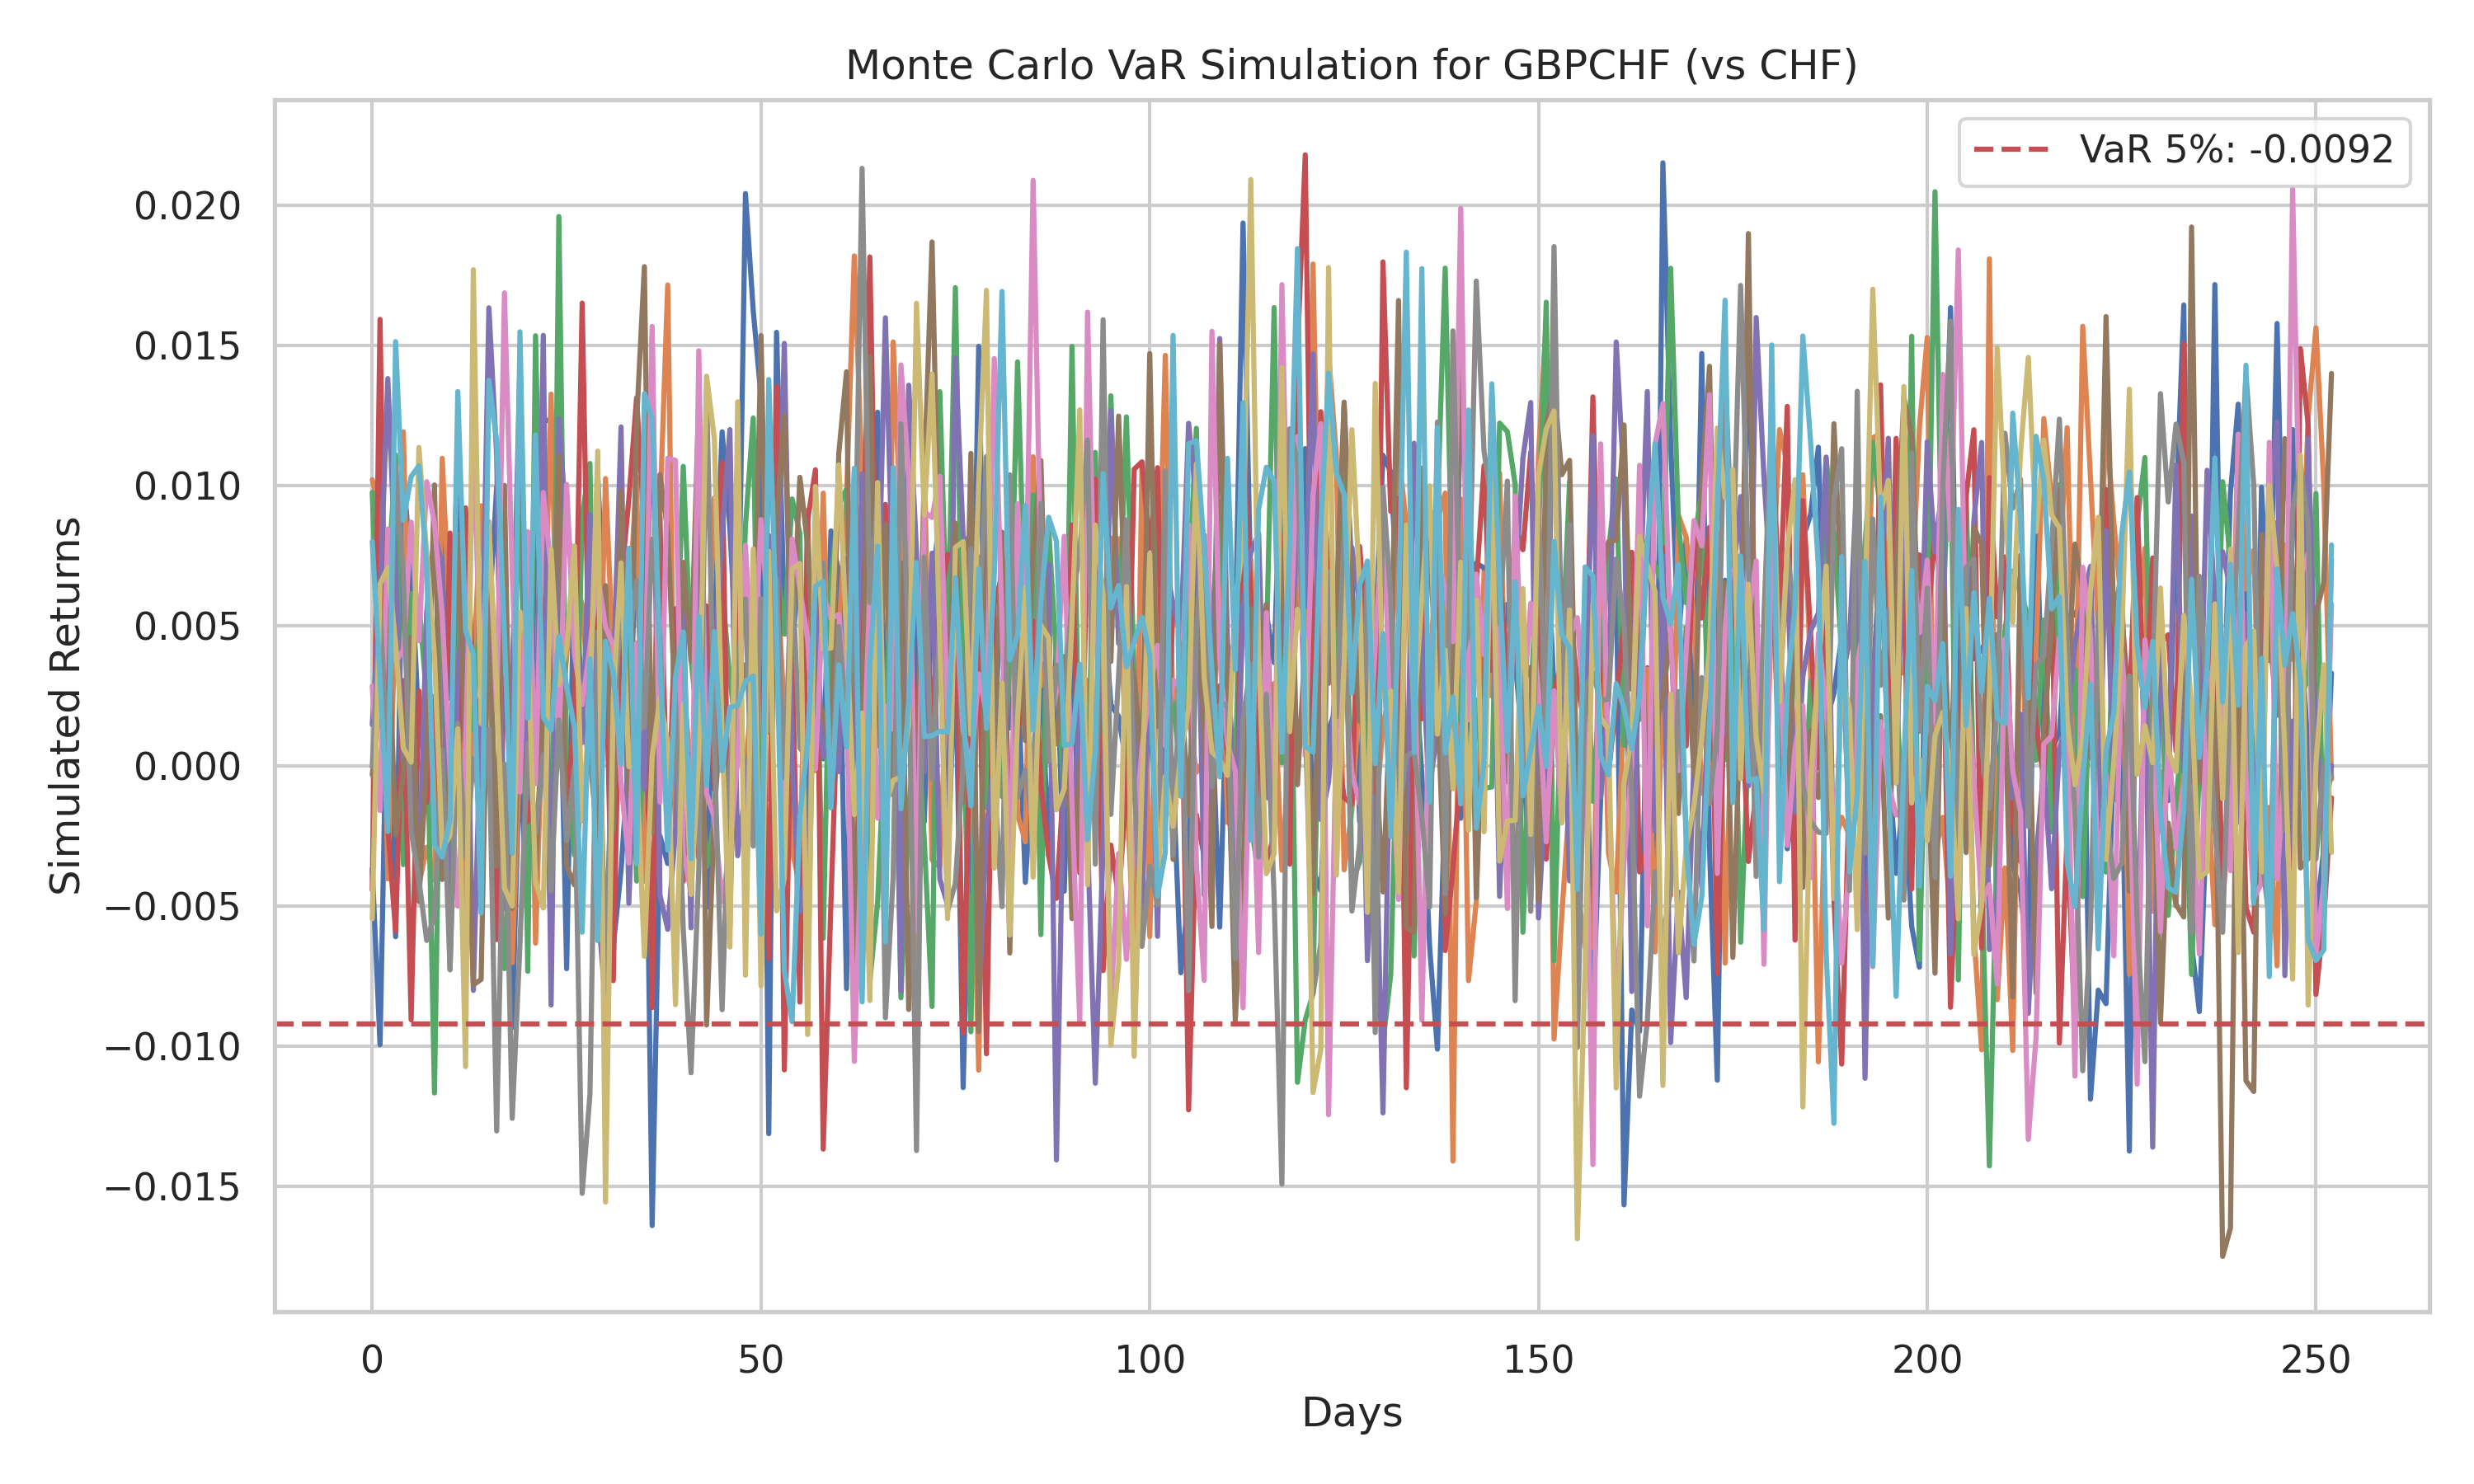
\includegraphics[width=0.7\linewidth]{../../reports/figures/monte_carlo_var_simulation_GBPCHF_vs_CHF.png} \label{fig:monte_carlo_var_simulation_GBPCHF_vs_CHF}
\end{figure}

\printbibliography
\end{document}
